%--------------------------------------------------------------------------
% Dokumentenklasse
%--------------------------------------------------------------------------

% disable Warning for remreset Package
% \RequirePackage{silence}
% \WarningFilter{remreset}{The remreset package}

\documentclass[
	pagesize,
	fontsize=12pt,
	paper=a4,
	oneside,
   reqno
]{scrartcl}

%--------------------------------------------------------------------------
% Standardpakete 
%--------------------------------------------------------------------------
\usepackage[ngerman]{babel}               % Deutsch Silbentrennung
\usepackage[T1]{fontenc}                  % Font Type
\usepackage[utf8]{inputenc}               % Font Encoding
\usepackage{lmodern}                      % Latin Modern Font
\usepackage{csquotes}                     % Setzen von Zitaten
\usepackage{xspace}                       % setzten von Leerzeichen nach Abkürzungen
\usepackage{microtype}                    % für glattere Seitenränder
\renewcommand*\familydefault{\sfdefault}  % Serifen lose Schrift
%\renewcommand*\familydefault{\ttdefault} % Schreibmaschinenschrift

%--------------------------------------------------------------------------
% Extra Packages
%--------------------------------------------------------------------------

% Abkürzungspaket
\usepackage{acronym}

% Symbolverzeichnis
\usepackage[symbols,nogroupskip,nonumberlist,sort=use]{glossaries-extra}

% \makenoidxglossaries

\glsxtrnewsymbol[description={Gewichtskraft}]{FG}{\ensuremath{F_{\mathrm{G}}}}
\glsxtrnewsymbol[description={Gewichtskraft in Bewegungsrichtung}]{FG1}{\ensuremath{F^{'}_{\mathrm{G}}}}
\glsxtrnewsymbol[description={Bewegungskraft des Schlittens}]{Fa}{\ensuremath{F_{\mathrm{a}}}}
\glsxtrnewsymbol[description={Pendelkraft}]{FP}{\ensuremath{F_{\mathrm{P}}}}
\glsxtrnewsymbol[description={Pendelkraft in Bewegungsrichtung}]{FP1}{\ensuremath{F^{'}_{\mathrm{P}}}}
\glsxtrnewsymbol[description={Reibkraft}]{Ff}{\ensuremath{F_{\mathrm{f}}}}
\glsxtrnewsymbol[description={Coulombsche Reibung}]{FC}{\ensuremath{F_{\mathrm{C}}}}
\glsxtrnewsymbol[description={Gesamtkraft}]{Fges}{\ensuremath{F_{\mathrm{ges}}}}
\glsxtrnewsymbol[description={Pendelmoment}]{MP}{\ensuremath{M_{\mathrm{P}}}}
\glsxtrnewsymbol[description={Gewichtsmoment}]{MG}{\ensuremath{M_{\mathrm{G}}}}
\glsxtrnewsymbol[description={Reibmoment}]{Mf}{\ensuremath{M_{\mathrm{f}}}}
\glsxtrnewsymbol[description={Gesamtmoment}]{Mges}{\ensuremath{M_{\mathrm{ges}}}}

% Mathe Pakete
\usepackage{amsmath}
\DeclareMathOperator{\sgn}{sgn}
\usepackage{thmtools}
\usepackage{amsfonts}
\usepackage{amssymb}
\usepackage{mathtools}
\usepackage{breqn}

% Listenumgebungen
\usepackage{listings}
\usepackage{paralist}
\usepackage{enumitem}
\usepackage{adjustbox}

% Demo Text
\usepackage{blindtext}

% Farb-Pakete
\usepackage{xcolor}
\usepackage{fancyvrb}
\usepackage{colortbl}

% Farbedefinitionen
\definecolor{htw}{RGB}{120, 184, 2}
\definecolor{ccW}{RGB}{255,255,255}
\definecolor{ccR}{RGB}{197,14,31}
\definecolor{ccG}{RGB}{113,113,113}
\definecolor{ccL}{RGB}{220,220,220}
\definecolor{ccS}{RGB}{0,0,0}
\definecolor{ccB}{RGB}{68,73,159}
\definecolor{ccD}{RGB}{0,0,80}

% Für erweiterte Tabellen
\usepackage{longtable}
\usepackage{tabularx}
\usepackage{float}
\usepackage{multirow}
\usepackage{makecell}
% \setlength{\tabcolsep}{0.5em}       % for the horizontal padding
% {\renewcommand{\arraystretch}{1.8}  % for the vertical padding
% \usepackage{ragged2e}
% \newcolumntype{R}[1]{>{\RaggedRight}p{#1}}

% Einheitenpaket
\usepackage[exponent-product = \cdot]{siunitx}
\sisetup{locale=DE}

\makeatletter
\renewcommand\@dotsep{5}
\makeatother

% Pakete für Grafiken
\usepackage{graphicx}
\usepackage{wrapfig}
\usepackage{overpic}
\usepackage{epstopdf}
\usepackage{caption}
\usepackage{subcaption}
\usepackage{rotating}
\usepackage{lscape}
% \captionsetup[subfigure]{list=true, font=normalsize, labelformat=brace, position=top} %setup für subfigure captions

% Diagramm-/Grafikerstellung
\usepackage{pstricks}
\usepackage{tikz}
\usetikzlibrary{math}
\usepackage{pgfplots}
\pgfplotsset{compat=1.5}
\usetikzlibrary{intersections,positioning,arrows,automata,calc,patterns,shapes.multipart,fit,backgrounds,decorations.pathreplacing}
\usetikzlibrary{decorations,shapes.geometric}
\usetikzlibrary{matrix,calc,angles,positioning,quotes}
% \usepackage{tikz-uml}

\usepackage{pgfkeys}
\usepackage{pgfopts}
\usepackage{ifthen}
\usepackage{xstring}
\usepackage{calc}
\usepackage{pst-plot,pst-bar,pst-node} % Balkendiagramme
\usepackage{capt-of}
\usepackage{incgraph} % Fullscreen Images
\usepackage{pdfpages} % Include external pdf pages

\usepackage{latexsym}
\usepackage{censor}
\usepackage{here}
% \StopCensoring        % Auskommentiert wird der Text entschwaerzt 
% \censor{Oszilloskop}  % Befehl zum einschwärzen
\usepackage{trfsigns}   % Transformation Symbol o---o \laplace and \Laplace
\usepackage{circuitikz}

\usepackage{multido}

% Verlinkungen im Text
\usepackage{url}
\usepackage{hyperref}
\PassOptionsToPackage{hyphens}{url}
\hypersetup{hidelinks}
\urlstyle{same}

%--------------------------------------------------------------------------
% Eigene Befehle
%--------------------------------------------------------------------------
% Test 
% \renewcommand{\thesection}{\arabic{section}} % Section startet mit 1.0 und nicht mit 0.1

%------------sectioning command-------------------
% The sectioning command one level down the hierarchy from \subsubsection is called \paragraph followed by \subparagraph
% to include this in your table of contents

% for paragraph
\setcounter{tocdepth}{4}
\setcounter{secnumdepth}{4}
% for subparagraph
\setcounter{tocdepth}{5}
\setcounter{secnumdepth}{5}

% Abkürzungen durch Kommandos setzen
\newcommand{\bspw}{bspw.\xspace}
\newcommand{\bzw}{bzw.\xspace}
\newcommand{\etc}{etc.\xspace}
\newcommand{\zB}{z.\,B.\xspace}
\newcommand{\EV}{e.\,V.\xspace}
\newcommand{\zT}{z.\,T.\xspace}
\newcommand{\iVm}{i.\,V.\,m.\xspace}
\newcommand{\idR}{i.\,d.\,R.\xspace}
\newcommand{\ihv}{i.\,H.\,v.\xspace}
\newcommand{\ua}{u.\,a.\xspace}
\newcommand{\dH}{d.\,h.\xspace}
\newcommand{\vgl}{vgl.\xspace}
\newcommand{\ca}{ca.\xspace}
\newcommand{\dV}{d.\,Verf.}
\newcommand{\RNr}{Rn.\xspace}
\newcommand{\oa}{o.\,{ä}.\xspace}
\newcommand{\vC}{v.\,Chr.\xspace}
\newcommand{\nC}{n.\,Chr.\xspace}
\newcommand{\vA}{v.\,a.\xspace}
\newcommand{\eng}{engl.\xspace}
\newcommand{\tabitem}{~~\llap{\textbullet}~~}

%------------Zitate-------------------------------
\newcommand*{\zitat}[2]{%
   \normalfont\small
   \begin{quote}
   \glqq#1\grqq \par
   #2
   \end{quote}
   \normalsize
}
\newcommand*{\zitatmitueberschrift}[3]{%
   \normalfont\small
   \begin{quote} #3
   \glqq#1\grqq \par
   #2
   \end{quote}
   \normalsize
}
\newcommand*{\zitext}[2]{%
   \glqq#1\grqq\ %
   [#2]%
}

%-----------Seitendesign--------------------------
\usepackage[width=15.5cm, height=23cm, includeheadfoot]{geometry}
\geometry{paper=a4paper}
% \usepackage[left=6cm,right=1cm,top=1.5cm, bottom=1cm, includeheadfoot]{geometry}
% \newgeometry{oneside}
% \setlength{\voffset}{0cm}
\setlength{\headheight}{1.1\baselineskip} % increase headheight
\setlength{\footheight}{28.99998pt}       % increase foodheight
\setlength{\parindent}{0cm}               % Einrücken nach \newline
\setlength{\footskip}{86pt}               % Move Footer down
% \setlength{\topmargin}{0cm}
% \setlength{\marginparsep}{0.5cm}
% \setlength{\marginparwidth}{1.5cm}
% \setlength{\textwidth}{16cm}
% \setlength{\textheight}{23cm}
% \setlength{\oddsidemargin}{1cm}
% \setlength{\evensidemargin}{2cm}

%----------Kopf & Fußzeile------------------------
% \usepackage[headsepline,footsepline]{scrpage2}
\usepackage[headsepline]{scrlayer-scrpage}
\pagestyle{scrheadings}
\clearpairofpagestyles
\ihead{\headmark}
\automark{section}
\chead{}
\ohead{
\includegraphics[scale=0.09]{Bilder/HTWLogoKopfzeile.png} \nocite{HTWklein}}
\ifoot{Sebastian Richter\\ Aaron Zielstorff}
\cfoot{\pagemark}
\ofoot{VA1 Moderne Methoden\\ der Regelungstechnik}

%--------------------------------------------------------------------------
% Beginn des Dokuments
%--------------------------------------------------------------------------
\begin{document}

%----------Deckblatt----------------------------- 
\begin{titlepage}
   \pagestyle{empty} % setzt Pagestyle-Befehl

   % HTW Logo
   \begin{flushright}
   
\includegraphics[scale=.07]{Bilder/LogoHTWBerlin.png}  \nocite{HTWgross}
   \end{flushright}

   \vspace{1cm}

   % Titel
   \begin{center}
      \Huge{\textbf{Inverses Pendel: Moderne Methoden der Regelungstechnik (VA1)}} \\
   \end{center}

   \vspace{3cm}

   % Name
   \begin{flushleft}
      \begin{tabular}{l c l }
         \textbf{Name: }&\hspace{1 cm} &\textbf{Matrikelnummer:} \\
         Sebastian Richter  & & 572906 \\
         Aaron Zielstorff   & & 567183 \\
      \end{tabular}
   \end{flushleft}

   \vspace{1cm}

   % Daten
   \begin{tabular}{l l}
      \textbf{Fachbereich:}   & FB1                                                 \\
      \textbf{Studiengang:}   & M.\xspace Elektrotechnik                            \\
      \textbf{Fachsemester:}  & 2.\xspace FS                                        \\
      \textbf{Fach:}          & VA1 Moderne Methoden der Regelungstechnik           \\
      \textbf{Dozent:}        & Prof.\xspace Dr.\xspace -Ing.\xspace Horst Schulte  \\
      \textbf{Abgabe am:}     & 19.\xspace Juli 2022                                \\ 
   \end{tabular}
\end{titlepage}
\clearpage

%--------Inhaltsverzeichnis-----------------------
\renewcommand{\contentsname}{Inhaltsverzeichnis}
\tableofcontents
\clearpage

%--------Abbildungsverzeichnis--------------------
\renewcommand{\listfigurename}{Abbildungsverzeichnis}
\renewcommand*{\figurename}{Abb.}
\listoffigures
% \clearpage

%--------Tabellenverzeichnis----------------------
\renewcommand*{\listtablename}{Tabellenverzeichnis}
\renewcommand*{\tablename}{Tab.}
\listoftables
\clearpage

%----------Symbolverzeichnis----------------------
% \printnoidxglossary[type=symbols,style=long,title={Symbolverzeichnis}]
% \clearpage

%---------Kapitel/Text----------------------------

\section{Einführung in die Regelaufgabe} \label{sec:Einfuehrung}

Photovoltaikanlagen enthalten viele Tausend einzelne Photovoltaikzellen. Jede Einzelne wandelt einfallende Sonnenstrahlung (direkt und indirekt) in elektrischen Strom um. Unter Vernachlässigung von Verlusten in Kabeln, Wandlerverlusten und Leistungsfehlanpassungen ist die erzeugte Leistung von PV-Systemen, die Anzahl aller enthaltenen Zellen multipliziert mit der Leistung einer einzelnen Zelle. Über diese Annahme ist es möglich, das mathematische Modell der gesamten PV-Anlage für die Systemanalyse abzuleiten. \\
Die Grundeinheiten einer PV-Anlage sind die PV-Module oder auch Solarzellen. Ein Standard-PV-Modul besteht aus 48 bis 73 in Reihe geschalteten Zellen, die in einen Rahmen montiert sind. PV-Anlagen werden in der Regel durch Reihen- und Parallelschaltungen von Modulen zusammengesetzt. Solarmodule werden in Reihe geschaltet (sog.\xspace \glqq Strings\grqq{}), um die Ausgangsspannung zu erhöhen. Parallel geschaltete Strings bilden ein \glqq Array\grqq{}, in dem die Leistungskapazität von Tausenden bis Millionen Watt aufgebaut werden kann. \\
Das mathematische Modell des PV-Generators ergibt sich aus der Zusammenfassung aller PV-Module, die durch das Modell einer einzelnen Zelle beschrieben werden. Strom und Spannung werden in geeigneter Weise multipliziert. Dazu wird die Einzelzelle durch ein Ersatzschaltbild modelliert, das aus einer einstrahlungsabhängigen Stromquelle, einem Modell der Diode $D$ und Shunt-Widerstand $R_{\mathrm{h}}$ besteht, wie in \autoref{fig:Bild1} (links) dargestellt. Die Einstrahlung $S$ mit der physikalischen Einheit $\SI{}{\frac{W}{m^2}}$ bezieht sich auf die direkte (normal zum PV-Zellenfeld) und die indirekte Einstrahlung. \\
\newline
Um die Spannung von PV-Anlagen zu regeln, werden Gleichspannungswandler eingesetzt. Die Ausgangsspannung des Wandlers kann eingestellt werden und unterscheidet sich von der Eingangsspannung. Eine grundlegende Gleichspannungswandlerschaltung ist der so genannte Buck Converter (Tiefsetzsteller), welcher ebenfalls in \autoref{fig:Bild1} (rechts) dargestellt ist. \\
Die Pulsweitenmodulation (PWM) ermöglicht die Steuerung und Regelung der gesamten Ausgangsspannung. Die PWM stellt ein Rechtecksignal bereit, welches zwischen 0 und 1 schaltet. Typische Schaltfrequenzen liegen zwischen $f_{\mathrm{SW}} = \SI{1}{kHz} \ldots \SI{1}{MHz}$. Im Falle der konkreten Anlage beträgt die Schaltfrequenz $f_{\mathrm{SW}} = \SI{5}{kHz}$. In der Praxis werden \zB MOSFET's als Schalter eingesetzt. Die Ausgangsspannung hinter dem MOSFET (siehe ebenfalls \autoref{fig:Bild1} (mittig)) wechselt somit zwischen Null und der Ausgangsspannung des Wandlers $v_{\mathrm{DC}}$. Das Tastverhältnis (Duty Cycle) $d$ beschreibt die Zeitverhältnisse des Rechtecksignals, also wann der Schalter (MOSFET) in Position 0 \bzw 1 ist. Der Duty Cycle lässt sich wie folgt berechnen:

\begin{align}
    d = \frac{v_{\mathrm{DC}}}{v_{\mathrm{PV}}} \quad \text{\bzw} \quad d = \frac{i_{\mathrm{PV}}}{i_{\mathrm{DC}}}
    \label{eq:Gleichung1}
\end{align}

Nachfolgend befindet sich die Darstellung der Modellparameter/Konstanten zur Modellierung des Buck Converters (siehe \autoref{tab:Tabelle1}).

\begin{table}[H]
    \centering
    \begin{tabular}{|lll|}
        \hline
        \rowcolor{grey}
        \textbf{Symbol}          & \textbf{Parameter}                               & \textbf{Wert}                            \\ \hline
        \rowcolor{lightGrey}
        \multicolumn{3}{|c|}{Standard Testbedingungen (STC)}                                                                   \\ \hline
        $T_{\mathrm{c,STC}}$     & PV Zelltemperatur bei STC                        & $\SI{298}{K}$                            \\
        $S_{\mathrm{STC}}$       & Bestrahlung bei STC                              & $\SI{1000}{\frac{W}{m^2}}$               \\
        $v_{\mathrm{T,STC}}$     & Thermische Spannung der p-n Sperrschicht bei STC & $\SI{25.7 \cdot 10^{-3}}{V}$             \\
        $i_{\mathrm{ph,sc,STC}}$ & Kurzschlussstrom des Diodenmodells bei STC       & $\SI{9.272}{A}$                          \\
        $v_{\mathrm{oc,STC}}$    & Leerlaufspannung bei STC                         & $\SI{0.644}{V}$                          \\ \hline
        \rowcolor{lightGrey}
        \multicolumn{3}{|c|}{Maximaler Leistungspunkt (MPP)}                                                                   \\ \hline
        $i_{\mathrm{PV,MPP}}$    & Gesamtstrom des PV Parks beim MPP                & $\SI{2902.13}{A}$                        \\
        $v_{\mathrm{PV,MPP}}$    & Gesamtspannung des PV Parks beim MPP             & $\SI{1049.13}{V}$                        \\
        $P_{\mathrm{MPP}}$       & Gesamtleistung des PV Parks beim MPP             & $\SI{30447.11}{W}$                       \\ \hline
        \rowcolor{lightGrey}
        \multicolumn{3}{|c|}{Weitere Parameter}                                                                                \\ \hline
        $R_{\mathrm{h}}$         & Shunt-Widerstand im Einzeldiodenmodell           & $\SI{10.196}{\Omega}$                    \\
        $v_{\mathrm{DC}}$        & Ausgangsgleichspannung                           & $\SI{900}{V}$                            \\
        $N_{\mathrm{cell,p}}$    & Anzahl paralleler Zellen pro Modul               & 1                                        \\
        $N_{\mathrm{cell,s}}$    & Anzahl serieller Zellen pro Modul                & 72                                       \\
        $N_{\mathrm{mod,p}}$     & Anzahl paralleler Module pro Anlage              & 336                                      \\
        $N_{\mathrm{mod,s}}$     & Anzahl serieller Module pro Anlage               & 27                                       \\
        $N_{\mathrm{p}}$         & Anzahl paralleler Zellen pro Anlage              & $\SI{336}{}$                             \\
        $N_{\mathrm{s}}$         & Anzahl serieller Zellen pro Anlage               & $\SI{1944}{}$                            \\
        $k$                      & Boltzmann Konstante                              & $\SI{1.381 \cdot 10^{-23}}{\frac{J}{K}}$ \\
        $q$                      & Elementarladung                                  & $\SI{1.602 \cdot 10^{-19}}{C}$           \\
        $A_{\mathrm{n}}$         & Dioden-Idealitätsfaktor im Einzeldiodenmodell    & $\SI{1.374}{}$                           \\
        $\alpha _{\mathrm{T}}$   & Temperaturkoeffizient des PV-Stroms              & $\SI{0.06 \cdot 10^{-2}}{}$              \\
        $\beta _{\mathrm{T}}$    & Temperaturkoeffizient der PV-Spannung            & $\SI{-0.36 \cdot 10^{-2}}{}$             \\ \hline
    \end{tabular}
    \caption{Modellparameter des Buck Converters}
    \label{tab:Tabelle1}
\end{table}

Ziel der Regelung soll es sein, die Ausgangsspannung $v_{\mathrm{DC}}$ konstant bei $\SI{900}{V}$ zu halten. Die einzelnen PV-Zellen wurden im Vorhinein für verschiedene Bestrahlungen und Temperaturen messtechnisch analysiert. Die nachfolgende Modellierung erfolgt zunächst für eine konstante Bestrahlung mit $S = \SI{1000}{\frac{W}{m^2}}$ bei einer konstanten Zelltemperatur von $T_{\mathrm{c}} = \SI{298}{K}$.

\begin{figure}[H]
   \centering
   \fbox{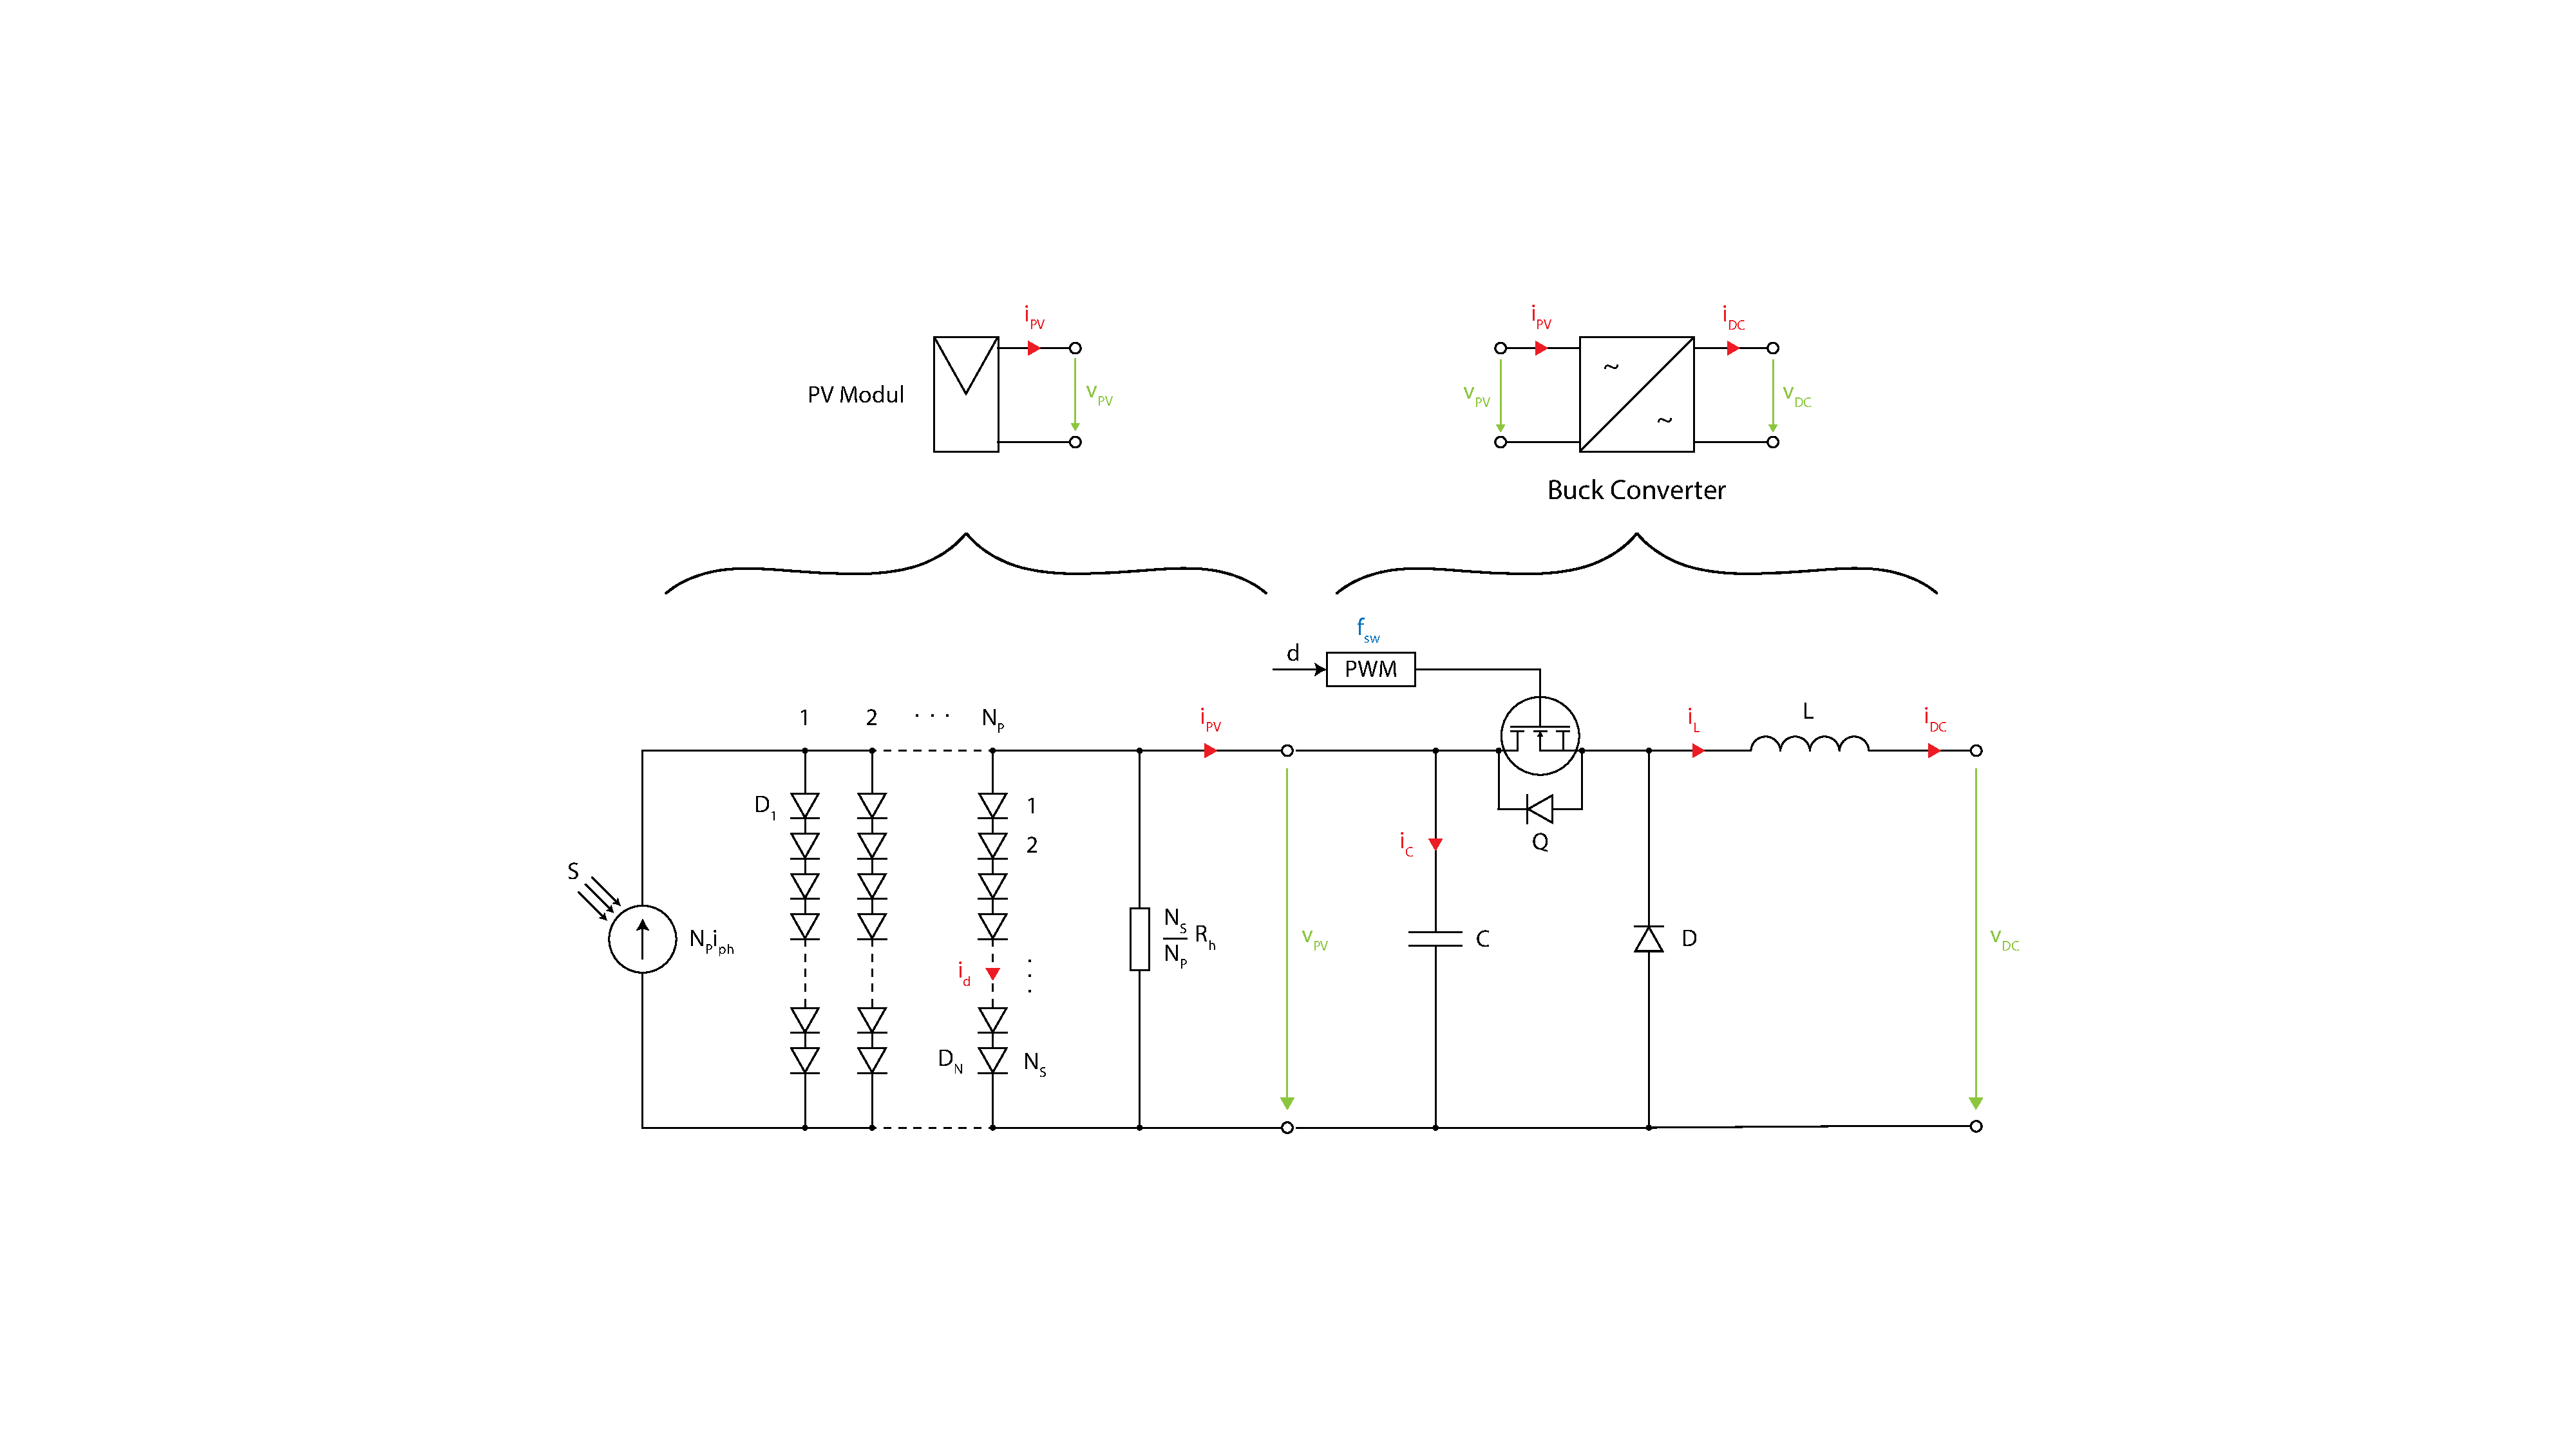
\includegraphics[width=1.0\textwidth]{Bilder/Buck_Zeichnung.pdf}}
   \caption[Skizze der Regelaufgabe]{Übersichtsschaltbild des Buck Converters als zu regelndes System inklusive Photovoltaik Anlage}
   \label{fig:Bild1}
\end{figure}

\section{Modellierung: Energiemethode nach Lagrange}

\subsection{Ansatz}

Die nachfolgende Gleichung zeigt den Lagrange Ansatz unter Berücksichtigung der dissipativen Funktion. Diese besagt in Erweiterung zu der Lagrange-Formulierung, dass Energie in einem Vorgang in Wärme umgewandelt wird. Mit Hilfe der dissipativen Funktion können Reibungsverluste bei der Energiemethode nach Lagrange berücksichtigt werden.

\begin{align} \label{eq:Gleichung1}
    \frac{d}{dt} \left(\frac{\partial L}{\partial \dot{q_{\mathrm{i}}}}\right) - \frac{\partial L}{\partial q_{\mathrm{i}}} + \frac{\partial D}{\partial \dot{q_{\mathrm{i}}}} = F_{\mathrm{i}}
\end{align}

\subsection{Freiheitsgrade und Zwangsbedingungen}

In \autoref{fig:Bild1} sind zwei Massepunkte im $\mathbb{R}^2$ zu erkennen. Somit gilt grundsätzlich:
\begin{itemize}
    \item 2 Punkte: 4 Freiheitsgrade (FHG)
\end{itemize}

Das inverse Pendel besitzt jedoch auch zwei Zwangsbedingungen, die wie folgt formuliert werden können:

\begin{itemize}
    \item Der Wagen kann sich nur horizontal bewegen: \\ $y_{\mathrm{M}} = 0$
    \item Die Masse $m$ am Ende des Pendels ist mit dem Wagen gekoppelt: \\ $(y_{\mathrm{M}} - y_{\mathrm{m}})^2 + (x_{\mathrm{M}} - x_{\mathrm{m}})^2 = l^2$
\end{itemize}

Somit bleiben am Ende noch zwei Freiheitsgrade (FHG) übrig.

\subsection{Generalisierte Koordinaten}

Aus den verbliebenen Freiheitsgraden werden die beiden generalisierten Koordinaten abgeleitet.

\begin{itemize}
    \item $q_{\mathrm{1}} = x_{\mathrm{M}}$
    \item $q_{\mathrm{2}} = \varphi$
\end{itemize}

\subsection{Berechnung der kinetischen und potentiellen Energie}

Der Ansatz zur Berechnung einer kinetischen Energie ist nachfolgend gezeigt.

\begin{align}\label{eq:Gleichung2}
    E_{\mathrm{kin}} = \frac{1}{2} \cdot m \cdot v^2
\end{align}

Zu berücksichtigen ist, dass beide Massen ($m$ und $M$) eine kinetische Energie besitzen (\autoref{eq:Gleichung3} und \autoref{eq:Gleichung4}).

\begin{align}
    E_{\mathrm{kin}} &= \frac{1}{2} \cdot M \cdot \dot{x}_{\mathrm{M}}^2 + \frac{1}{2} \cdot m \cdot v_{\mathrm{m}}^2 \label{eq:Gleichung3} \\
    E_{\mathrm{kin}} &= \frac{1}{2} \cdot M \cdot \dot{x}_{\mathrm{M}}^2 + \frac{1}{2} \cdot m \cdot \left(\dot{x}_{\mathrm{m}}^2 + \dot{y}_{\mathrm{m}}^2\right) \label{eq:Gleichung4}
\end{align}

Weiter gilt:

\begin{align*}
    x_{\mathrm{m}} &= x_{\mathrm{M}} + l \cdot \sin({\varphi}) \\
    y_{\mathrm{m}} &= l \cdot \cos({\varphi}) \\
    \dot{x_{\mathrm{m}}} &= \dot{x_{\mathrm{M}}} + l \cdot \dot{\varphi} \cdot \cos{\varphi} \\
    \dot{y_{\mathrm{m}}} &= -l \cdot \dot{\varphi} \cdot \sin({\varphi})
\end{align*}

Daraus resultiert:

\begin{dmath*}
    E_{\mathrm{kin}} = \frac{1}{2} \cdot M \cdot \dot{x}_{\mathrm{M}}^2 + \frac{1}{2} \cdot m \cdot \left(\left(\dot{x}_{\mathrm{M}} + l \cdot \dot{\varphi} \cdot \cos({\varphi})\right)^2 + \left( -l \cdot \dot{\varphi} \cdot \sin({\varphi})\right)^2\right) \\
    = \frac{1}{2} \cdot M \cdot \dot{x}_{\mathrm{M}}^2 + \frac{1}{2} \cdot m \cdot \left(\dot{x}_{\mathrm{M}}^2 + 2 \cdot \dot{x}_{\mathrm{M}} \cdot l \cdot \dot{\varphi} \cdot \cos({\varphi}) + l^2 \cdot \dot{\varphi}^2 \cdot \cos^2(\varphi) + l^2 \cdot \dot{\varphi}^2 \cdot \sin^2(\varphi)\right) \\
    = \frac{1}{2} \cdot M \cdot \dot{x}_{\mathrm{M}}^2 + \frac{1}{2} \cdot m \cdot \dot{x}_{\mathrm{M}}^2 + m \cdot \dot{x}_{\mathrm{M}} \cdot l \cdot \dot{\varphi} \cdot \cos({\varphi}) + \frac{1}{2} \cdot m \cdot l^2 \cdot \dot{\varphi}^2 \cdot \cos^2(\varphi) + \frac{1}{2} \cdot m \cdot l^2 \cdot \dot{\varphi}^2 \cdot \sin^2(\varphi)
\end{dmath*}

Durch das Zusammenfassen der vorangegangenen Beziehung folgt \autoref{eq:Gleichung5} für die gesamte kinetische Energie des Systems.

\begin{align} \label{eq:Gleichung5}
    E_{\mathrm{kin}} = \frac{1}{2} \cdot \dot{x}_{\mathrm{M}}^2 \cdot (M + m) + \frac{1}{2} \cdot m \cdot \left( 2 \cdot \dot{x}_{\mathrm{M}} \cdot l \cdot \dot{\varphi} \cdot \cos({\varphi}) + l^2 \cdot \dot{\varphi}^2\right)
\end{align}

Ausschließlich die Masse $m$ am Pendelende besitzt eine für den Lagrange-Formalismus relevante potentielle Energie (\autoref{eq:Gleichung6}).

\begin{align}
    E_{\mathrm{pot}} &= m \cdot g \cdot h \nonumber \\
    E_{\mathrm{pot}} &= m \cdot g \cdot y_{\mathrm{m}} \nonumber \\
    E_{\mathrm{pot}} &= m \cdot g \cdot l \cdot \cos({\varphi}) \label{eq:Gleichung6}
\end{align}

\subsection{Herleitung der Bewegungsgleichungen}

Die Lagrange-Funktion wird aus der Differenz der kinetischen und der potentiellen Energie berechnet (\autoref{eq:Gleichung7}).

\begin{align} 
        L &= E_{\mathrm{kin}} - E_{\mathrm{pot}}  \label{eq:Gleichung7} \\ 
        L &= \frac{1}{2} \cdot \dot{x}_{\mathrm{M}}^2 \cdot (M + m) + \frac{1}{2} \cdot m \cdot \left( 2 \cdot \dot{x}_{\mathrm{M}} \cdot l \cdot \dot{\varphi} \cdot \cos({\varphi}) + l^2 \cdot \dot{\varphi}^2\right) - m \cdot g \cdot l \cdot \cos({\varphi}) \label{eq:Gleichung8}
\end{align}

Im ersten Schritt wird die Bewegungsgleichung des Wagens hergeleitet. Dafür wird zunächst \autoref{eq:Gleichung8} nach der ersten zeitlichen Ableitung der generalisierten Koordinate $x_{\mathrm{M}}$ partiell differenziert:

\begin{align}\label{eq:Gleichung9}
    \frac{\partial L}{\partial \dot{x}_{\mathrm{M}}} = (M + m) \cdot \dot{x}_{\mathrm{M}} + m \cdot l \cdot \dot{\varphi} \cdot \cos(\varphi)
\end{align}

Die vorangegangene Gleichung wird zeitlich differenziert:

\begin{align}\label{eq:Gleichung10}
    \frac{d}{dt}\left(\frac{\partial L}{\partial \dot{x}_{\mathrm{M}}}\right) = (M + m) \cdot \ddot{x}_{\mathrm{M}} + m \cdot l \cdot \left(\ddot{\varphi} \cdot \cos(\varphi) - \dot{\varphi}^2 \cdot \sin(\varphi) \right)
\end{align}

Im zweiten Schritt wird die Lagrange-Funktion nach der generalisierten Koordinate $x_{\mathrm{M}}$ abgeleitet.

\begin{align}\label{eq:Gleichung11}
    \frac{\partial L}{\partial x_{\mathrm{M}}} = 0
\end{align}

Abschließend wird die dissipative Funktion nach der 1. Ableitung der generalisierten Koordinate $x_{\mathrm{M}}$ differenziert.

\begin{align}\label{eq:Gleichung12}
    \frac{\partial D}{\partial \dot{x_{\mathrm{M}}}} = d \cdot \dot{x_{\mathrm{M}}}
\end{align}

Durch das Einsetzen der \autoref{eq:Gleichung9} bis \autoref{eq:Gleichung12} in den Ansatz aus \autoref{eq:Gleichung1} resultiert die vollständige Bewegungsgleichung des Wagens.

\begin{align}\label{eq:Gleichung13}
    (M + m) \cdot \ddot x_{\mathrm{M}} + m \cdot l \cdot \left( \ddot \varphi \cdot \cos({\varphi}) - \dot \varphi^2 \cdot \sin({\varphi})\right) + d \cdot \dot x_{\mathrm{M}} = F_{\mathrm{a}}
\end{align}

Analog wird die Bewegungsgleichung des Pendels entwickelt. Hierbei wird zunächst \autoref{eq:Gleichung8} nach der 1. Ableitung der generalisierten Koordinate $\varphi$ partiell differenziert.

\begin{align}\label{eq:Gleichung14}
    \frac{\partial L}{\partial \dot{\varphi}} = m \cdot l \cdot \dot{x}_{\mathrm{M}} \cdot \cos(\varphi) + m \cdot l^2 \cdot \dot{\varphi}
\end{align}

Die vorangegangene Gleichung wird nach der Zeit abgeleitet:

\begin{align}\label{eq:Gleichung15}
    \frac{d}{dt}\left(\frac{\partial L}{\partial \dot{\varphi}}\right) = m \cdot l \cdot \left(\ddot{x}_{\mathrm{M}} \cdot  \cos(\varphi) - \dot{x}_{\mathrm{M}} \cdot \sin(\varphi) \cdot \dot{\varphi}\right) + m \cdot l^2 \cdot \ddot{\varphi}
\end{align}

Als nächstes wird für die Bewegungsgleichung des Pendels die Lagrange-Funktion nach der generalisierten Koordinate $\varphi$ abgeleitet:

\begin{align}\label{eq:Gleichung16}
    \frac{\partial L}{\partial \varphi} = -m \cdot l \cdot \dot{\varphi} \cdot \dot{x}_{\mathrm{M}} \cdot \sin(\varphi) + m \cdot g \cdot l \cdot \sin(\varphi)
\end{align}

Abschließend wird die dissipative Funktion analog nach der 1. Ableitung der generalisierten Koordinate $\varphi$ differenziert:

\begin{align}\label{eq:Gleichung17}
    \frac{\partial D}{\partial \dot{\varphi}} = d_{\mathrm{Mf}} \cdot \dot{\varphi}
\end{align}

Über das Anwenden von \autoref{eq:Gleichung1} folgt die Bewegungsgleichung des Pendels zu:

\begin{align}\label{eq:Gleichung18}
    \ddot{x}_{\mathrm{M}} \cdot \cos(\varphi) + l \cdot \ddot{\varphi} - g \cdot \sin(\varphi) + \frac{d_{\mathrm{Mf}} \cdot \dot{\varphi}}{m \cdot l} = 0
\end{align}

\section{Nichtlineares Zustandsraummodell}

\subsection{Umformungen}

Zum Aufstellen des nichtlinearen Zustandsraummodells werden die \autoref{eq:Gleichung13} und \autoref{eq:Gleichung18} nach den höchsten Ableitungen $\ddot x_{\mathrm{M}}$ und $\ddot \varphi$ umgestellt.

\begin{align}
    \ddot x_{\mathrm{M}} &= \frac{-d_{\mathrm{Mf}} \cdot \dot \varphi -m \cdot l^2 \cdot \ddot \varphi + m \cdot g \cdot l \cdot \sin({\varphi})}{m \cdot l \cdot \cos({\varphi})} \label{eq:Gleichung19} \\
    \ddot \varphi &= \frac{F_{\mathrm{a}} - (M+m) \cdot \ddot x_{\mathrm{M}} + m \cdot l \cdot \dot \varphi^2 \cdot \sin({\varphi}) -d \cdot \dot x_{\mathrm{M}}}{m \cdot l \cdot \cos({\varphi})} \label{eq:Gleichung20}
\end{align}
\newline
Beide Gleichungen sind über die Wagenbeschleunigung $\ddot x_{\mathrm{M}}$ und der Winkelbeschleunigung $\ddot \varphi$ miteinander verkoppelt. Durch das gegenseitige Einsetzen werden die Abhängigkeiten eliminiert.

\begin{align}
    \ddot x_{\mathrm{M}} &= \frac{-d_{\mathrm{Mf}} \cdot \dot \varphi -m \cdot l^2 \cdot \left( \frac{F_{\mathrm{a}} - (M+m) \cdot \ddot x_{\mathrm{M}} + m \cdot l \cdot \dot \varphi^2 \cdot \sin({\varphi}) -d \cdot \dot x_{\mathrm{M}}}{m \cdot l \cdot \cos({\varphi})} \right) + m \cdot g \cdot l \cdot \sin({\varphi})}{m \cdot l \cdot \cos({\varphi})} \label{eq:Gleichung21} \\
    \ddot \varphi &= \frac{F_{\mathrm{a}} - (M+m) \cdot \left( \frac{-d_{\mathrm{Mf}} \cdot \dot \varphi -m \cdot l^2 \cdot \ddot \varphi + m \cdot g \cdot l \cdot \sin({\varphi})}{m \cdot l \cdot \cos({\varphi})} \right) + m \cdot l \cdot \dot \varphi^2 \cdot \sin({\varphi}) -d \cdot \dot x_{\mathrm{M}}}{m \cdot l \cdot \cos({\varphi})} \label{eq:Gleichung22}
\end{align}

\subsection{Zustandsraumdarstellung (nichtlinear)}

Das zu untersuchende System weist vier Zustände auf, welche in Form eines Zustandsvektors $\underline{x}$ erfasst werden (siehe \autoref{eq:Gleichung24}). Die Dokumentation der zeitlichen Ableitungen erfolgt im Vektor der Zustandsänderungen $\dot{\underline{x}}$ (siehe \autoref{eq:Gleichung25}). Der Eingangsvektor $\underline{u}$ gleicht der Eingangskraft des Systems $F_{\mathrm{a}}$, wie in \autoref{eq:Gleichung23} gezeigt wird.

\begin{align}\label{eq:Gleichung23}
    \underline{u} &= F_{\mathrm{a}}
\end{align}
\newline
Der Zustandsvektor ergibt sich zu:

\begin{align}
    \underline{x} &=
    \begin{bmatrix}\label{eq:Gleichung24}
        x_{\mathrm{1}} \\
        x_{\mathrm{2}} \\
        x_{\mathrm{3}} \\
        x_{\mathrm{4}}
    \end{bmatrix} =
    \begin{bmatrix}
        \varphi         \\
        \dot \varphi    \\
        x_{\mathrm{M}}  \\
        \dot x_{\mathrm{M}}
    \end{bmatrix}
\end{align}

Nach zeitlicher Ableitung des Zustandsvektors ergibt sich Der Vektor der Zustandsänderungen zu:
\begin{align}\label{eq:Gleichung25}
    \dot{\underline{x}} &=
    \begin{bmatrix}
        \dot x_{\mathrm{1}} \\
        \dot x_{\mathrm{2}} \\
        \dot x_{\mathrm{3}} \\
        \dot x_{\mathrm{4}}
    \end{bmatrix} =
    \begin{bmatrix}
        \dot{\varphi}           \\
        \ddot{\varphi}          \\
        \dot{x}_{\mathrm{M}}    \\
        \ddot{x}_{\mathrm{M}}
    \end{bmatrix}
\end{align}
\newline
Mithilfe der \autoref{eq:Gleichung23} bis \autoref{eq:Gleichung25}, durch das Einsetzen in \autoref{eq:Gleichung21} und \autoref{eq:Gleichung22}, dem Zusammenfassen und Umstellen nach $\ddot x_{\mathrm{M}}$ und $\ddot \varphi$ folgt das \textbf{nichtlineare Zustandsraummodell} aus \autoref{eq:Gleichung26}.

\begin{empheq}[box=\widefbox]{align} \label{eq:Gleichung26}
    \dot{\underline{x}} =
    \begin{bmatrix}
        x_2 \\
        \frac{\left(\frac{F_{\mathrm{a}} - g \cdot \tan(x_{\mathrm{1}}) \cdot (M + m) - d \cdot x_{\mathrm{4}}}{m \cdot l \cdot \cos(x_{\mathrm{1}})} + d_{\mathrm{Mf}} \cdot x_{\mathrm{2}} \cdot \left(\frac{M}{m^2 \cdot l^2 \cdot \cos^2(x_{\mathrm{1}})} + \frac{1}{m \cdot l^2 \cdot \cos^2(x_{\mathrm{1}})}\right) + x_{\mathrm{2}}^2 \cdot \tan(x_{\mathrm{1}})\right)}{\left(1 - \frac{1}{\cos^2(x_{\mathrm{1}})} - \frac{M}{m \cdot \cos^2(x_{\mathrm{1}})}\right)} \\
        x_{\mathrm{4}} \\
        \frac{\left(g \cdot \tan(x_{\mathrm{1}}) - \frac{F_{\mathrm{a}}}{m \cdot \cos^2(x_{\mathrm{1}})} + \frac{d \cdot x_{\mathrm{4}}}{m \cdot \cos^2(x_{\mathrm{1}})} - \frac{l \cdot x_{\mathrm{2}}^2 \cdot \tan(x_{\mathrm{1}})}{\cos(x_{\mathrm{1}})} - \frac{d_{\mathrm{Mf}} \cdot x_{\mathrm{2}}}{m \cdot l \cdot \cos(x_{\mathrm{1}})}\right)}{\left(1 - \frac{(M + m)}{m \cdot \cos^2(x_{\mathrm{1}})}\right)}
    \end{bmatrix}
\end{empheq}

\section{Linearisiertes Zustandsraummodell}

\subsection{Linearisierungsvorschrift}

Das Verhalten des nichtlinearen Systems ist für große Änderungen des Eingangssignals nicht vorhersehbar. Um dennoch Aussagen über das Systemverhalten treffen zu können, wird das nichtlineare Zustandsraummodell mithilfe der Taylorreihenentwicklung um eine Ruhelage ($\underline{x}^{*}$) linearisiert. Die nichtlinearen Restglieder $\underline{R}(\Delta{\underline{x}^2}, \Delta{\underline{u}^2})$ werden zu Null angenommen. Durch die Linearisierung wird das Systemverhalten für kleine Änderungen um die Ruhelage kontrollierbar. Nachfolgend ist die Taylorreihenentwicklung für Linearisierung aufgeführt:

\begin{align} \label{eq:Gleichung27}
    \begin{split}
        \dot{\underline{x}}^{*}+\Delta{\dot{\underline{x}}} &=\underline{f}(\underline{x}^{*}+\Delta{\underline{x}},\underline{u}^{*}+\Delta{\underline{u}})\\
        &=\underline{f}(\underline{x}^{*},\underline{u}^{*})+\left[\frac{\partial f_{\mathrm{i}}}{\partial x_{\mathrm{j}}}\right]_{(\underline{x}^{*}, \underline{u}^{*})}\cdot\Delta{\underline{x}}+\left[\frac{\partial f_{\mathrm{i}}}{\partial u_{\mathrm{j}}}\right]_{(\underline{x}^{*},\underline{u}^{*})}\cdot\Delta{\underline{u}}+\underline{R}(\Delta{\underline{x}^2}, \Delta{\underline{u}^2})
    \end{split}
\end{align}
\newline
Durch die Annahme über das Verhalten der nichtlinearen Restglieder folgt die Struktur des linearen Zustandsraummodells dargestellt in \autoref{eq:Gleichung28}

\begin{align} \label{eq:Gleichung28}
    \begin{split}
        \Delta\dot{\underline{x}} &= \left[\frac{\partial f_{\mathrm{i}}}{\partial x_{\mathrm{j}}}\right]_{(\underline{x}^{*}, \underline{u}^{*})}\cdot\Delta{\underline{x}}+\left[\frac{\partial f_{\mathrm{i}}}{\partial u_{\mathrm{j}}}\right]_{(\underline{x}^{*},\underline{u}^{*})}\cdot\Delta{\underline{u}}\\   
        \Delta{\underline{y}} &= \left[\frac{\partial h_{\mathrm{i}}}{\partial x_{\mathrm{j}}}\right]_{(\underline{x}^{*}, \underline{u}^{*})}\cdot\Delta{\underline{x}}+\left[\frac{\partial h_{\mathrm{i}}}{\partial u_{\mathrm{j}}}\right]_{(\underline{x}^{*},\underline{u}^{*})}\cdot\Delta{\underline{u}}
    \end{split}
\end{align}
\newline
mit:

\begin{align*}
    \Delta\underline{x} &= \underline{x} - \underline{x}_{\mathrm{c}} \\
    \Delta \underline{u} &= \underline{u} - \underline{F}_{\mathrm{a}}.
\end{align*}
\newline
Die Variablen $\underline{x}_{\mathrm{c}}$ und $\underline{F_{a}}$ beschreiben die Ruhelagen des Systems. Allgemein gefasst wird das \textbf{lineare Zustandsraummodell} folgendermaßen dargestellt:

\begin{empheq}[box=\widefbox]{align} \label{eq:Gleichung29}
    \begin{split}
        \dot{\underline{x}} &= \underline{A}\cdot\underline{x}+\underline{B}\cdot\underline{u} \\
        \underline{y} &= \underline{C}\cdot\underline{x}+\underline{D}\cdot\underline{u}
    \end{split}
\end{empheq}

\subsection{Stabile und instabile Ruhelage}

Um das linearisierte Zustandsraummodell zu erhalten, werden die einzelnen Gleichungen des nichtlinearen Zustandsraummodells aus \autoref{eq:Gleichung26} nach den Zuständen $x_{\mathrm{1}}$ bis $x_{\mathrm{4}}$, sowie dem Eingang $F_{\mathrm{a}}$ partiell abgeleitet und die entsprechende Ruhelage eingesetzt. Dabei werden zwei Ruhelagen Betrachtet. Nachfolgend dargestellt ist die Ruhelage des hängenden Pendels (untere Ruhelage):

\begin{align}\label{eq:Gleichung30}
    \begin{split}
        \underline{x}_{\mathrm{1}}^{*}=
        \begin{bmatrix}
            x_{\mathrm{1}}^{*}\\
            x_{\mathrm{2}}^{*}\\
            x_{\mathrm{3}}^{*}\\
            x_{\mathrm{4}}^{*}
        \end{bmatrix}=
        \begin{bmatrix}
            Pi\\
            0\\
            0\\
            0
        \end{bmatrix}
    \end{split}
\end{align}
\newline
Die Regelung soll dafür sorgen, dass das Pendel in der stehenden (oberen) Ruhelage verweilt. Diese wird beschrieben durch:

\begin{align}\label{eq:Gleichung31}
    \begin{split}
        \underline{x}_{\mathrm{2}}^{*}=
        \begin{bmatrix}
            x_{\mathrm{1}}^{*}\\
            x_{\mathrm{2}}^{*}\\
            x_{\mathrm{3}}^{*}\\
            x_{\mathrm{4}}^{*}
        \end{bmatrix}=
        \begin{bmatrix}
            0\\
            0\\
            0\\
            0
        \end{bmatrix}
    \end{split}
\end{align}

\subsection{Zustandsraumdarstellung (linear)}

Unter der Berücksichtigung der oberen Ruhelage ergibt sich das \textbf{linearisierte Zustandsraummodell} für das hängende Pendel zu:

\begin{empheq}[box=\widefbox]{align} \label{eq:Gleichung32}
    \begin{split}
        \Delta{\dot{\underline{x}}}&=
        \begin{bmatrix}
            0 & 1 & 0 & 0 \\
            -26.6505 & -0.0248 & 0 & -5.8333 \\
            0 & 0 & 0 & 1 \\
            -0.8502 & -7.916\cdot10^-4 & 0 & -2.333
        \end{bmatrix}\cdot\Delta\underline{x}+
        \begin{bmatrix}
            0 \\
            0.8333 \\
            0 \\
            0.3333
        \end{bmatrix}\cdot F_{\mathrm{a}}
        \\
        \Delta{\underline{y}} &=
        \begin{bmatrix}
            1 & 0 & 0 & 0 \\
            0 & 0 & 1 & 0 \\
            0 & 0 & 0 & 1
        \end{bmatrix}\cdot\Delta\underline{x}+\underline{0}\cdot F_{\mathrm{a}}
    \end{split}
\end{empheq}

\clearpage

Wird die obere Ruhelage herangezogen folgt das \textbf{linearisierte Zustandsraummodell} zu:

\begin{empheq}[box=\widefbox]{align} \label{eq:Gleichung33}
    \begin{split}
        \Delta{\dot{\underline{x}}}&=
        \begin{bmatrix}
            0 & 1 & 0 & 0 \\
            26.6505 & -0.0248 & 0 & 5.8333 \\
            0 & 0 & 0 & 1 \\
            -0.8502 & 7.916\cdot10^-4 & 0 & -2.333
        \end{bmatrix}\cdot\Delta\underline{x}+
        \begin{bmatrix}
            0 \\
            -0.8333 \\
            0 \\
            0.3333
        \end{bmatrix}\cdot F_{\mathrm{a}}
        \\
        \Delta{\underline{y}} &=
        \begin{bmatrix}
            1 & 0 & 0 & 0 \\
            0 & 0 & 1 & 0 \\
            0 & 0 & 0 & 1
        \end{bmatrix}\cdot\Delta\underline{x}+\underline{0}\cdot F_{\mathrm{a}}
    \end{split}
\end{empheq}

\subsection{Überprüfung der Steuerbarkeit} \label{sec:Steuerbarkeit}

Die Steuerbarkeit eines Systems ist gegeben, wenn unter Berücksichtigung der Eingangsgröße $\underline{u}(t)$ das System von einem Anfangszustand $\underline{x}_{\mathrm{0}}$ in einen beliebigen Endzustand $\underline{x}_{\mathrm{e}}$ gebracht werden kann. Dies wird mathematisch für quadratische Matrizen mithilfe der Determinante, und für nicht-quadratische Matrizen mit dem Rang der Steuerbarkeitsmatrix $Q_{\mathrm{s}}$ nachgewiesen. Die Berechnung der Steuerbarkeitsmatrix erfolgt durch \autoref{eq:Gleichung34}.

\begin{align}\label{eq:Gleichung34}
    \underline{Q}_{\mathrm{s}} &= \left(\underline{B} \quad \underline{A}\cdot\underline{B} \quad ... \quad \underline{A}^{(n-1)}\cdot\underline{B}\right)
\end{align}
\newline
Zur Überprüfung werden die System- und Eingangsmatrix des linearisierten Modells um die instabile Ruhelage (stehendes Pendel) eingesetzt. Die Steuerbarkeitsmatrix $Q_{\mathrm{s}}$ ist quadratisch, d.h. die Determinante muss ungleich Null sein. Die \textbf{Steuerbarkeitsmatrix des Systems} wurde berechnet zu:

\begin{align}\label{eq:Gleichung35}
    \underline{Q}_{\mathrm{s}} &=
    \begin{bmatrix}
        0 & -0.8333 & 1.9651 & -26.7984 \\
        -0.8333 & 1.9651 & -26.7984 & 67.7740 \\
        0 & 0.3333 & -0.7784 & 2.5264 \\
        0.3333 & -0.7784 & 2.5264 & -7.5869
    \end{bmatrix}
\end{align}
\newline
Die \textbf{Determinante} folgt zu

\begin{equation*}
    \boxed{det(\underline{Q}_{\mathrm{s}}) = 46.41 \neq 0},
\end{equation*}
\newline
womit das System nachgewiesen \textbf{steuerbar} ist.

\section{Vergleich beider Systeme} \label{sec:systemvergleich}

Der Vergleich des Systemverhaltens des nichtlinearen (\autoref{fig:Bild2}) und des linearen Systems (\autoref{fig:Bild3}) wird in der stabilen Ruhelage durchgeführt, da hierzu keine Reglerstruktur benötigt wird. Der Vergleich wird auf Grundlage der Winkellage durchgeführt. Für den direkten Vergleich wird zu jedem Zeitpunkt ein radialer Winkel Pi zu dem Winkel $\varphi$ des linearen Systems addiert. Als Testsignal wird ein Einheitssprung nach 0.5s mit der Amplitude Eins eingeprägt.

\begin{figure}[H]
   \centering
   \fbox{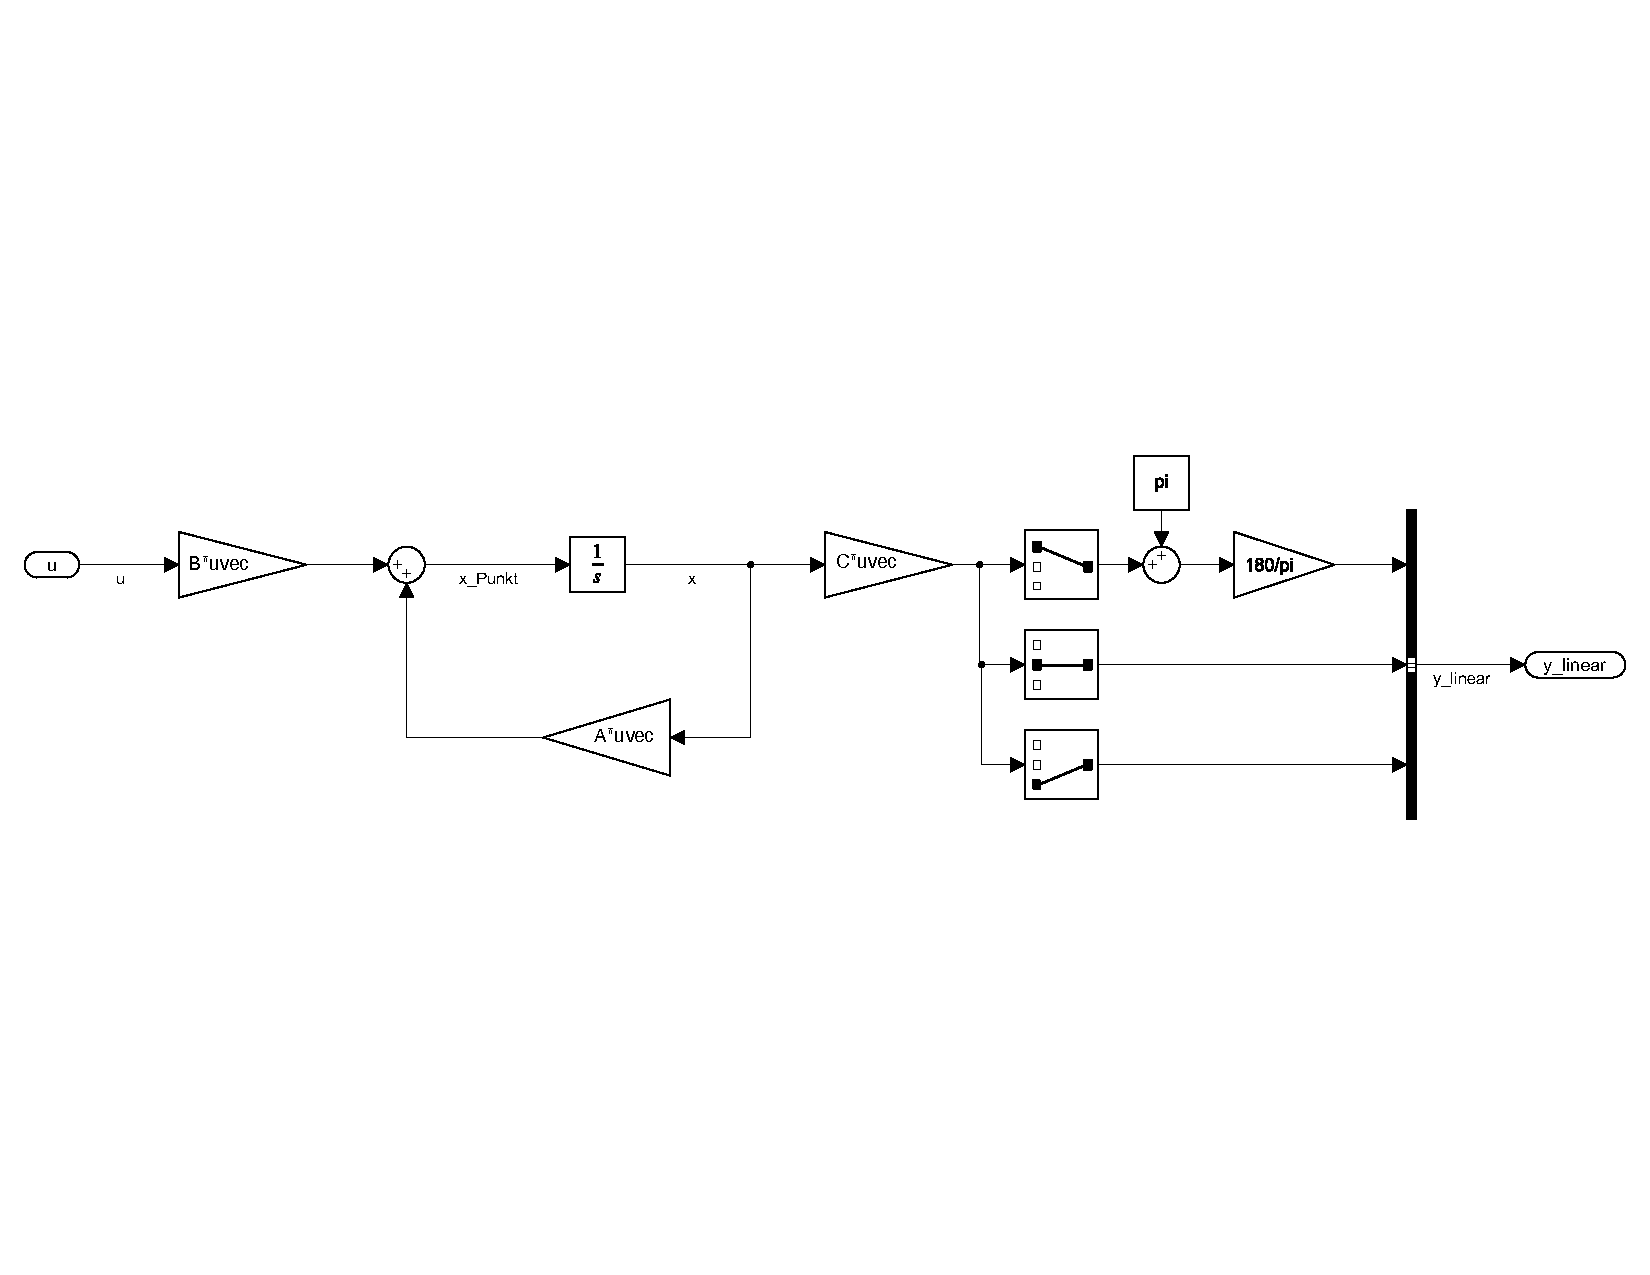
\includegraphics[width=0.85\textwidth]{Bilder/Lineare_Strecke.pdf}}
   \caption[Simulink-Modell des nichtlinearen Systems]{Simulink-Modell des nichtlinearen Systems}
   \label{fig:Bild2}
\end{figure}

\begin{figure}[H]
   \centering
   \fbox{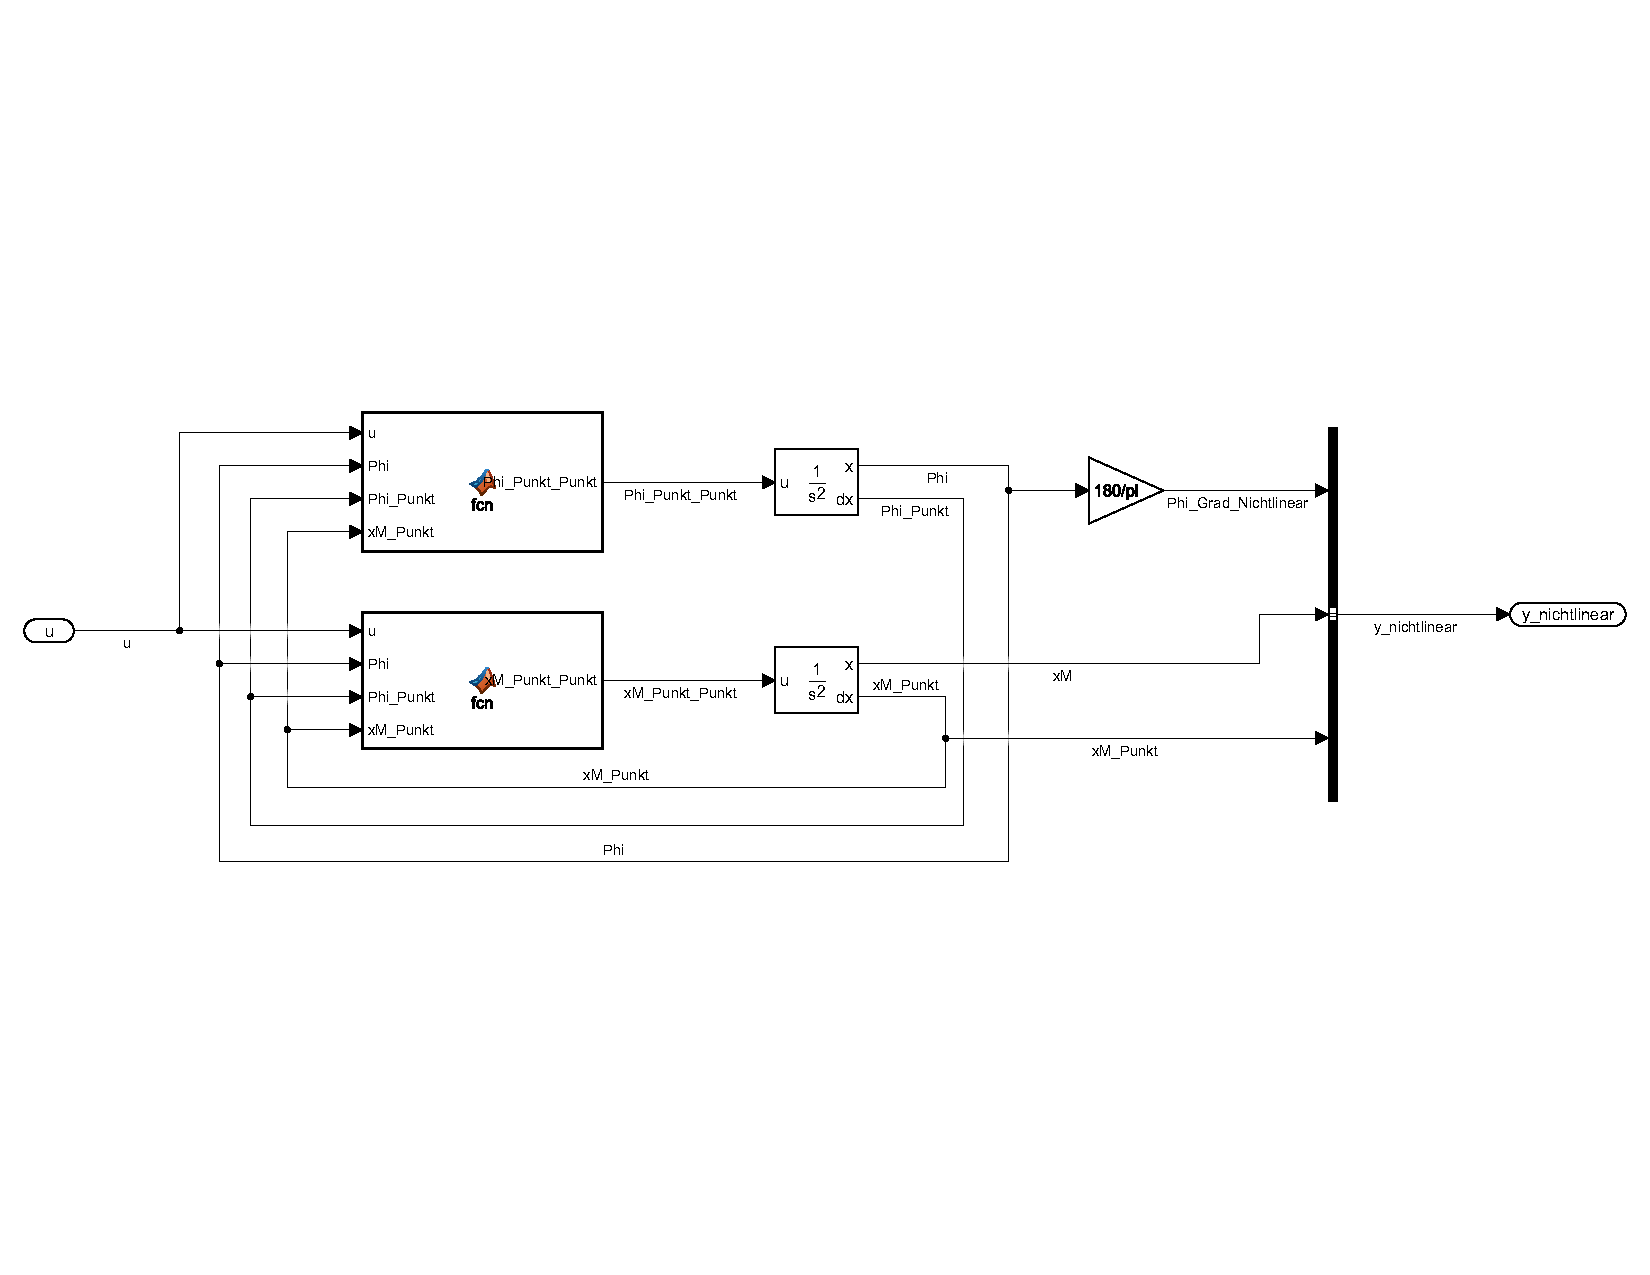
\includegraphics[width=0.85\textwidth]{Bilder/Nichtlineare_Strecke.pdf}}
   \caption[Simulink-Modell des linearisierten Systems]{Simulink-Modell des linearisierten Systems}
   \label{fig:Bild3}
\end{figure}

Beim Vergleich der beiden Systemverhalten ist zu erkennen, dass diese für kleine Winkelauslenkungen nahezu identisch erscheinen (\autoref{fig:Bild4} und \autoref{fig:Bild5}). Durch den sinusoidalen Signalverlauf wird weiter geschlussfolgert, dass eine positive Eingangskraft (Wagen fährt nach rechts) das Pendel in positive Winkelrichtung ausschlagen lässt. Da keine weiteren äußeren Kräfte auf das System eingeprägt werden, erfolgt mit steigender Zeit t durch die Reib- und Dämpfungsmomente das erneute Einpendeln in die stabile Ruhelage (hängendes Pendel).

\begin{figure}[H]
   \centering
   \fbox{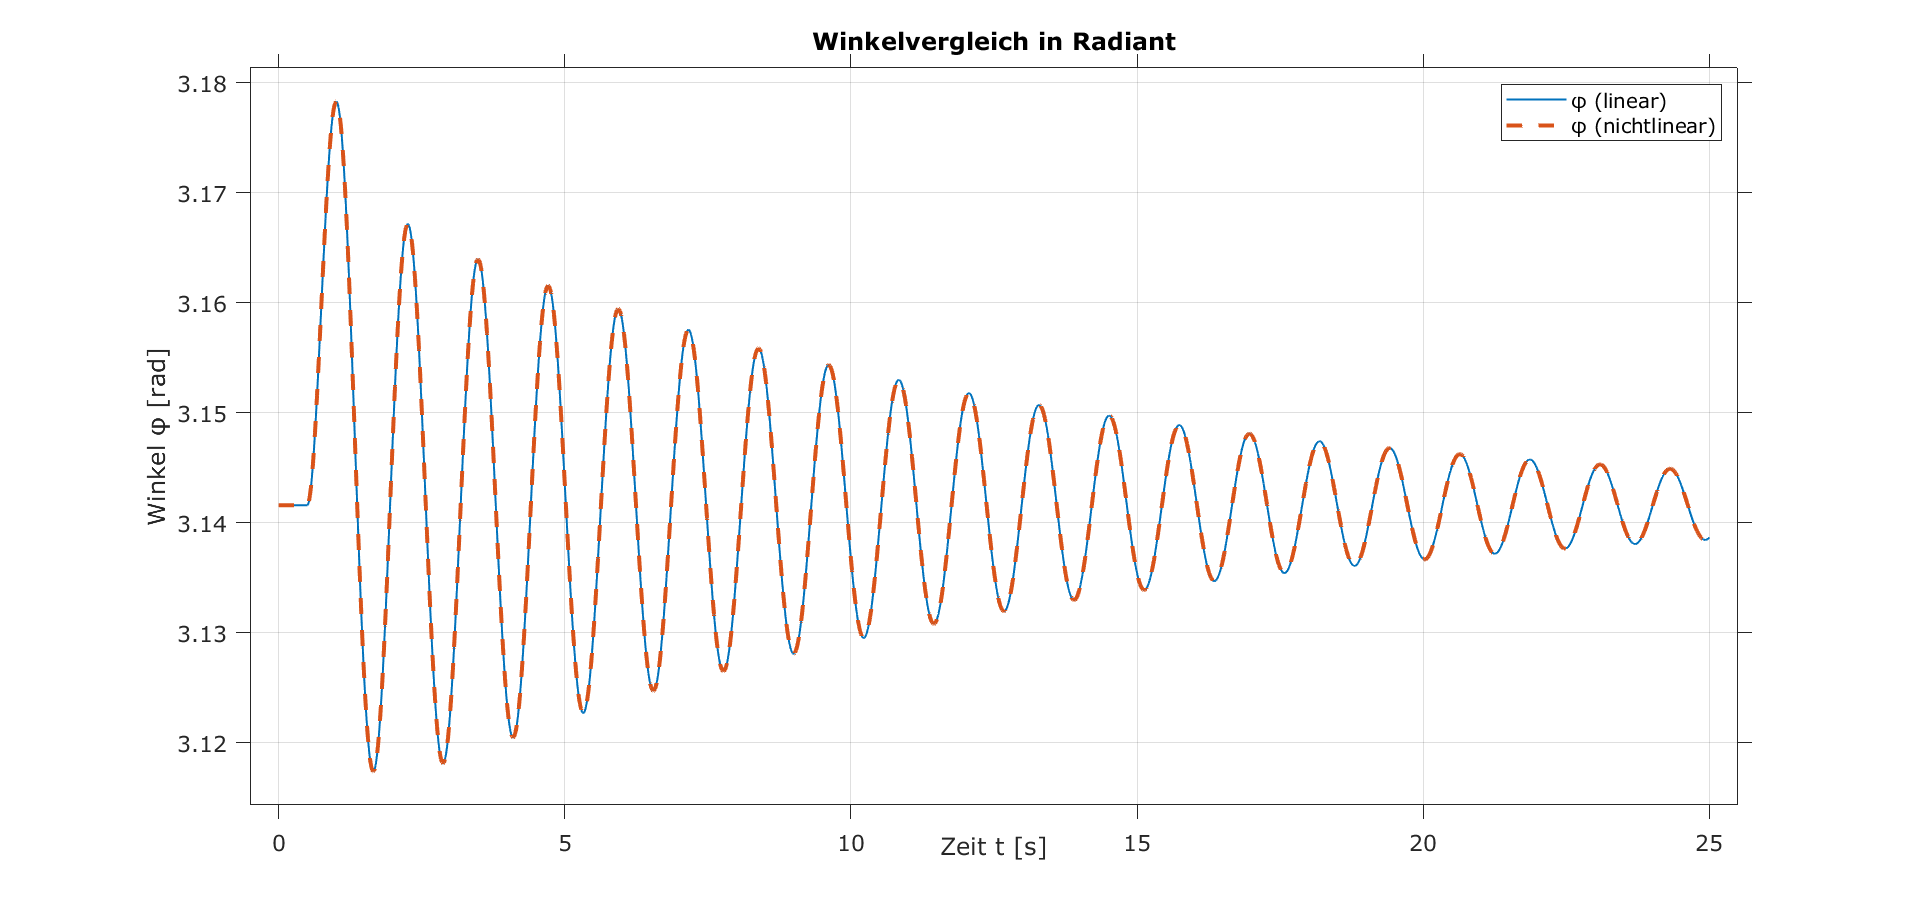
\includegraphics[width=0.9\textwidth]{Bilder/Phi_rad_Vergleich.png}}
   \caption[Vergleich der beiden radialen Winkelverläufe]{Vergleich der beiden radialen Winkelverläufe}
   \label{fig:Bild4}
\end{figure}

\begin{figure}[H]
    \centering
    \fbox{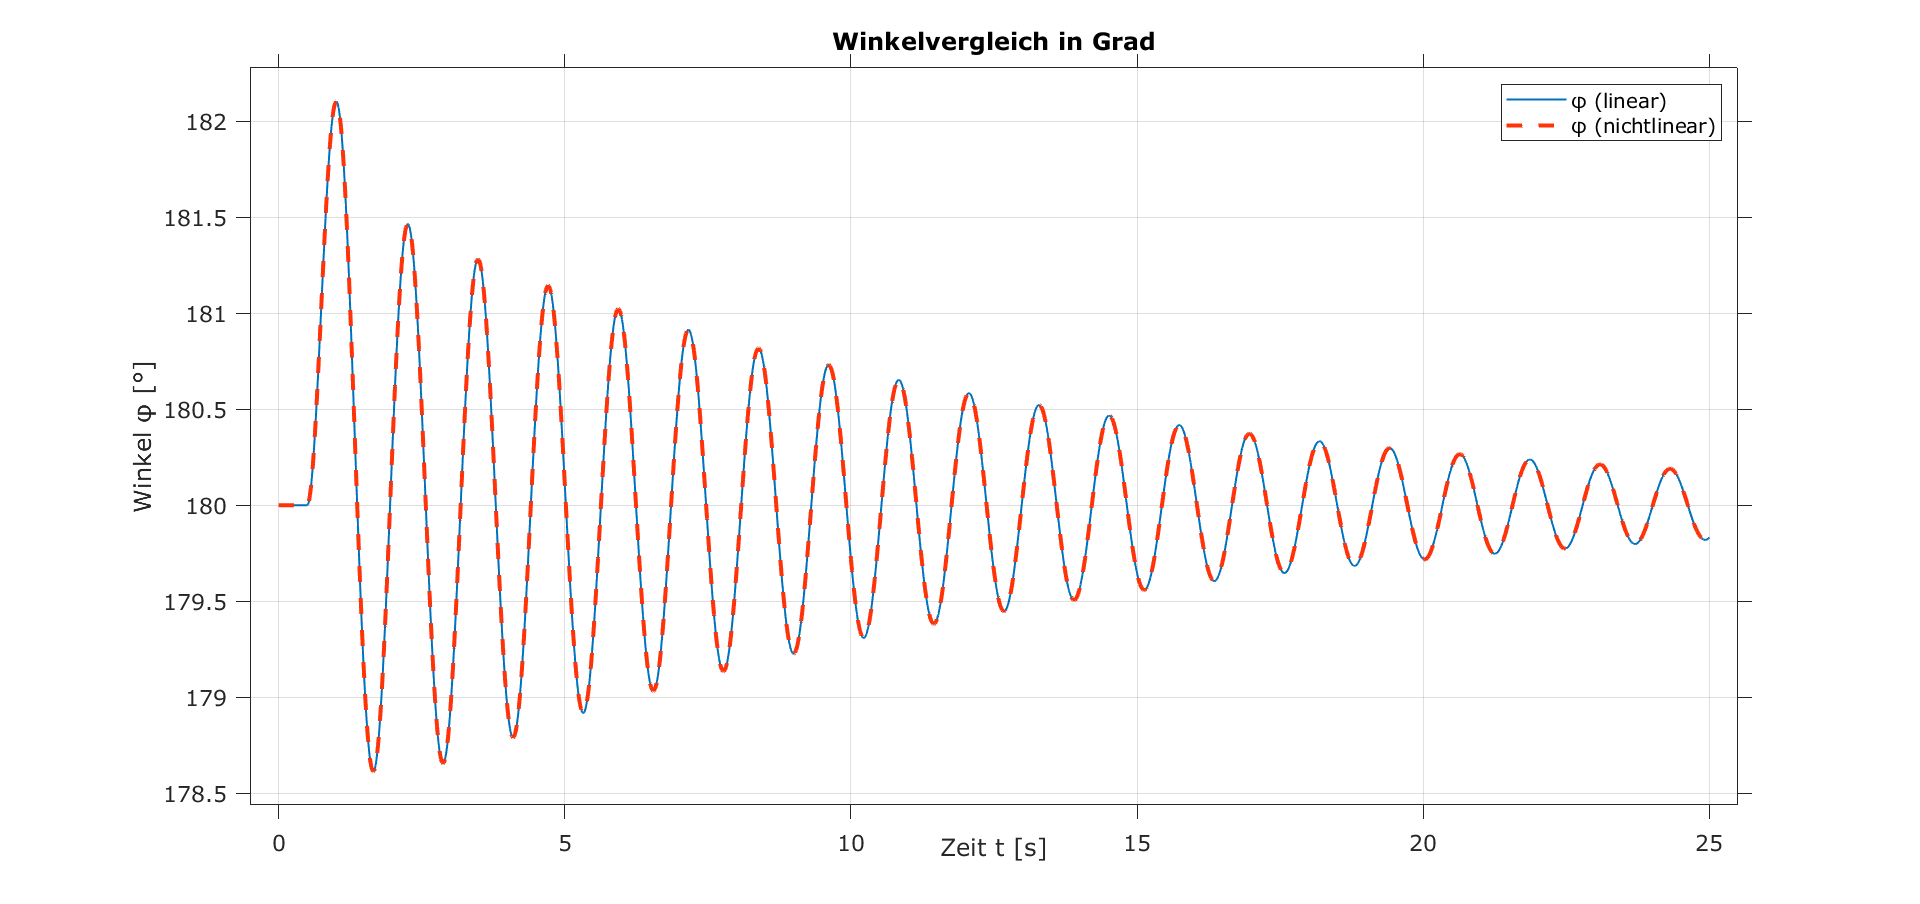
\includegraphics[width=0.9\textwidth]{Bilder/Phi_Grad_Vergleich.png}}
    \caption[Vergleich der beiden Winkelverläufe in Grad]{Vergleich der beiden Winkelverläufe in Grad}
    \label{fig:Bild5}
\end{figure}

Wird die Eingangskraft $F_{\mathrm{a}}$, welche auf das System wirkt, signifikant vergrößert (Einheitssprung mit Amplitude 15), werden größere Winkelauslenkungen erreicht. Dies führt zur Verringerung der Zuverlässigkeit des linearisierten Systems und zu Abweichungen zwischen dem linearen und nichtlinearem Systemverhalten (\autoref{fig:Bild6}).

\begin{figure}[H]
    \centering
    \fbox{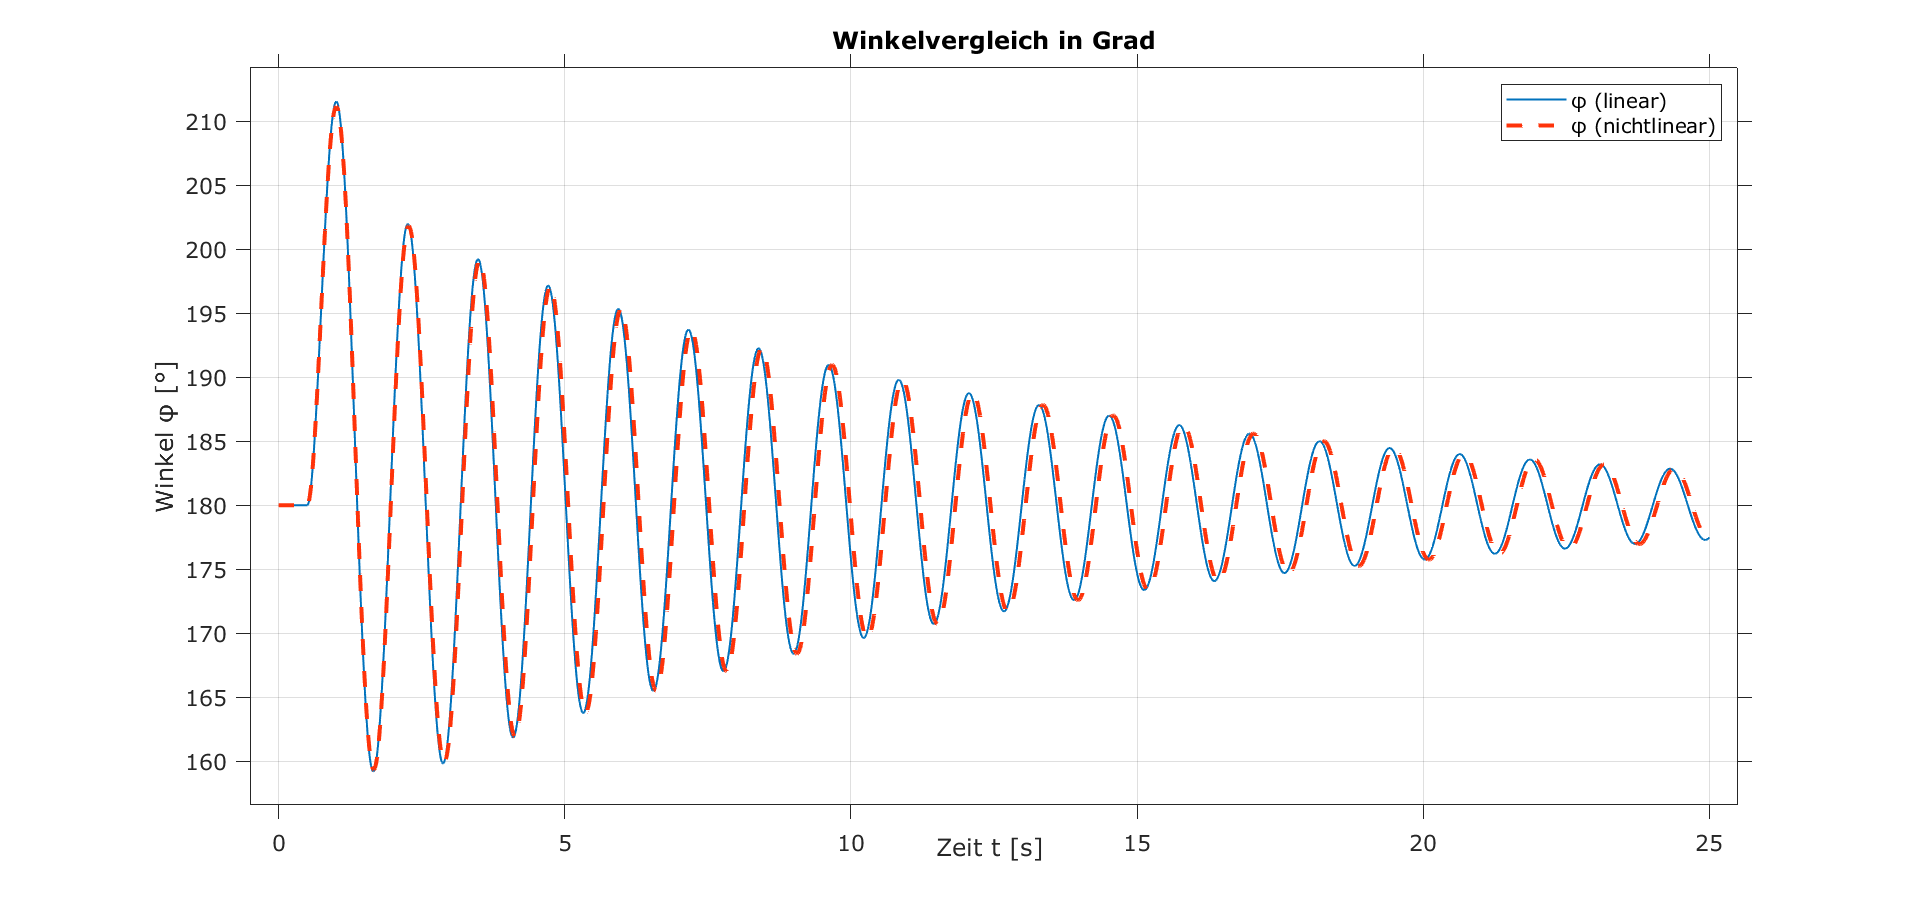
\includegraphics[width=0.9\textwidth]{Bilder/Phi_Grad_Vergleich_Verschiebung.png}}
    \caption[Vergleich der beiden Winkelverläufe in Grad mit Abweichung]{Abweichungen im Systemverhalten für größere Winkelauslenkungen}
    \label{fig:Bild6}
\end{figure}

\section{Zustandsreglerentwurf} \label{sec:Zustandsreglerentwurf}

\subsection{Einfache Zustandsrückführung} \label{sec:Ackermann-Formel}

Die erste umgesetzte Regelstrategie ist die einfache Zustandsrückführung unter Anwendung der \textbf{Ackermann-Formel für Systeme mit einem Eingang}. Ziel ist es, das Pendel-System mit einem Anfangswinkel ungleich Null Grad erneut in die instabile Ruhelage zu bringen. Dafür werden mit Hilfe der Ackermann-Formel k-Faktoren berechnet, welche anschließend mit den Zuständen $x_{\mathrm{1}}$ bis $x_{\mathrm{4}}$ multipliziert und auf den Systemeingang zurückgeführt werden (\autoref{fig:Bild7}). Der Wagen wird dabei immer in den Ausgangszustand von $x_{\mathrm{M}}$ zurück geregelt.

\begin{figure}[H]
    \centering
    \fbox{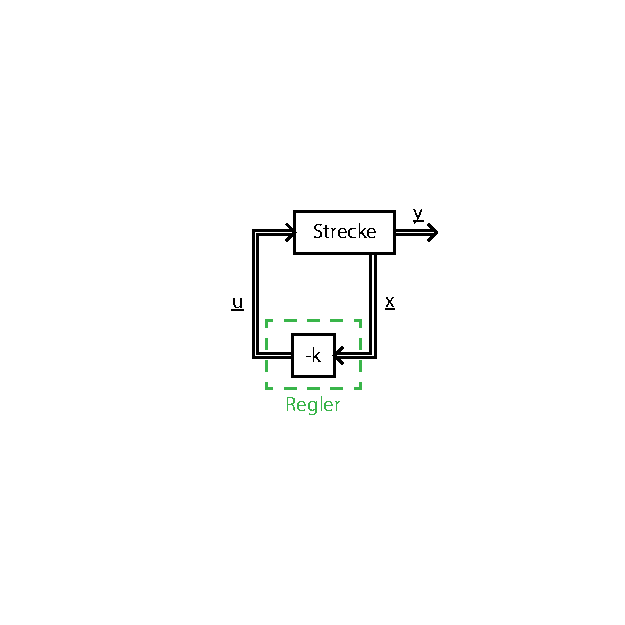
\includegraphics[width=0.3\textwidth]{Bilder/Ackermann.pdf}}
    \caption[Reglerstruktur einfache Zustandsrückführung]{Schematische Darstellung der Reglerstruktur der einfachen Zustandsrückführung}
    \label{fig:Bild7}
\end{figure}

Im ersten Schritt wird der Nachweis der Steuerbarkeit des Systems benötigt. Dieser wurde bereits in \autoref{sec:Steuerbarkeit} erbracht.
Im zweiten Schritt erfolgt die Bestimmung der Eigenwerte der Systemmatrix A. Hierzu wird das charakteristische Polynom benötigt, welches mithilfe der Laplace-Transformation der Vektorzustandsdifferentialgleichungen $\underline{\dot{x}}$ und der anschließenden Umformung hergeleitet wird.

\begin{align*}
    \underline{\dot{x}} &= \underline{A}\cdot\underline{x}+\underline{B}\cdot\underline{u}\quad\laplace \quad s\cdot \underline{X}(s)-\underline{x}_{\mathrm{0}}=\underline{A}\cdot \underline{X}(s)+\underline{B}\cdot \underline{U}(s) \\
    \underline{X}(s) &= (s\cdot \underline{I} - \underline{A})^{-1}\cdot\underline{x}_{\mathrm{0}}+(s\cdot \underline{I} - \underline{A})^{-1}\cdot\underline{B}\cdot\underline{U}(s)
\end{align*}
\newline
Das charakteristische Polynom folgt aus der Determinante von ($s\cdot\underline{I}-\underline{A}$). Die Matrix $\underline{I}$ stellt die Einheitsmatrix dar. Die Nullstellen des Polynoms gleichen den Eigenwerte der Systemmatrix A. Das \textbf{Charakteristische Polynom} und Eigenwertdefinition ist nachfolgend dargestellt:

\begin{align*}
    \underline{P}(s) &= det(s\cdot\underline{I}-\underline{A}) \\
    \underline{P}(s_{\mathrm{P}}) &= \underline{0} = eig(\underline{A})
\end{align*}
\newline
Allgemeine Form:

\begin{align*}
        \underline{P}(s) &= s^n+\alpha_{n-1}\cdot s^{\mathrm{n-1}}+...+\alpha_{\mathrm{1}}\cdot s + \alpha_{\mathrm{0}} \\
        \underline{P}(s) &= (s-s_{\mathrm{P1}})\cdot(s-s_{\mathrm{P2}})\cdot ... \cdot (s-s_{\mathrm{Pn}})
\end{align*}
\newline
Die Berechnung der Eigenwerte der Systemmatrix erfolgt analog zu den vorangegangenen Betrachtungen. Die \textbf{Eigenwerte des Systems} ergeben sich zu:

\begin{empheq}[box=\widefbox]{align} \label{eq:Gleichung36}
    eig(\underline{A}) &= eig
    \begin{bmatrix}
        0 & 1 & 0 & 0 \\
        26.6505 & -0.0248 & 0 & 5.8333 \\
        0 & 0 & 0 & 1 \\
        -0.8502 & 7.916\cdot10^-4 & 0 & -2.333
    \end{bmatrix} \nonumber\\
    eig(\underline{A}) &=
    \begin{bmatrix}
        0 \\
        5.0852 \\
        -5.3333 \\
        -2.1100
    \end{bmatrix}
\end{empheq}
\newline
Die Eigenwerte müssen einen negativen Realteil aufweisen, andernfalls ist das System instabil. Die Polstellen des Reglers werden auf $s_{\mathrm{P}} = -4+0j$ festgelegt (\autoref{eq:Gleichung37}). Die Lage aller \textbf{Polstellen} ist in \autoref{fig:Bild8} visualisiert.

\begin{empheq}[box=\widefbox]{align} \label{eq:Gleichung37}
    \underline{s}_{\mathrm{P}} &= 
    \begin{bmatrix}
        -4 & -4 & -4 & -4 
    \end{bmatrix}
\end{empheq}

\begin{figure}[H]
    \centering
    \fbox{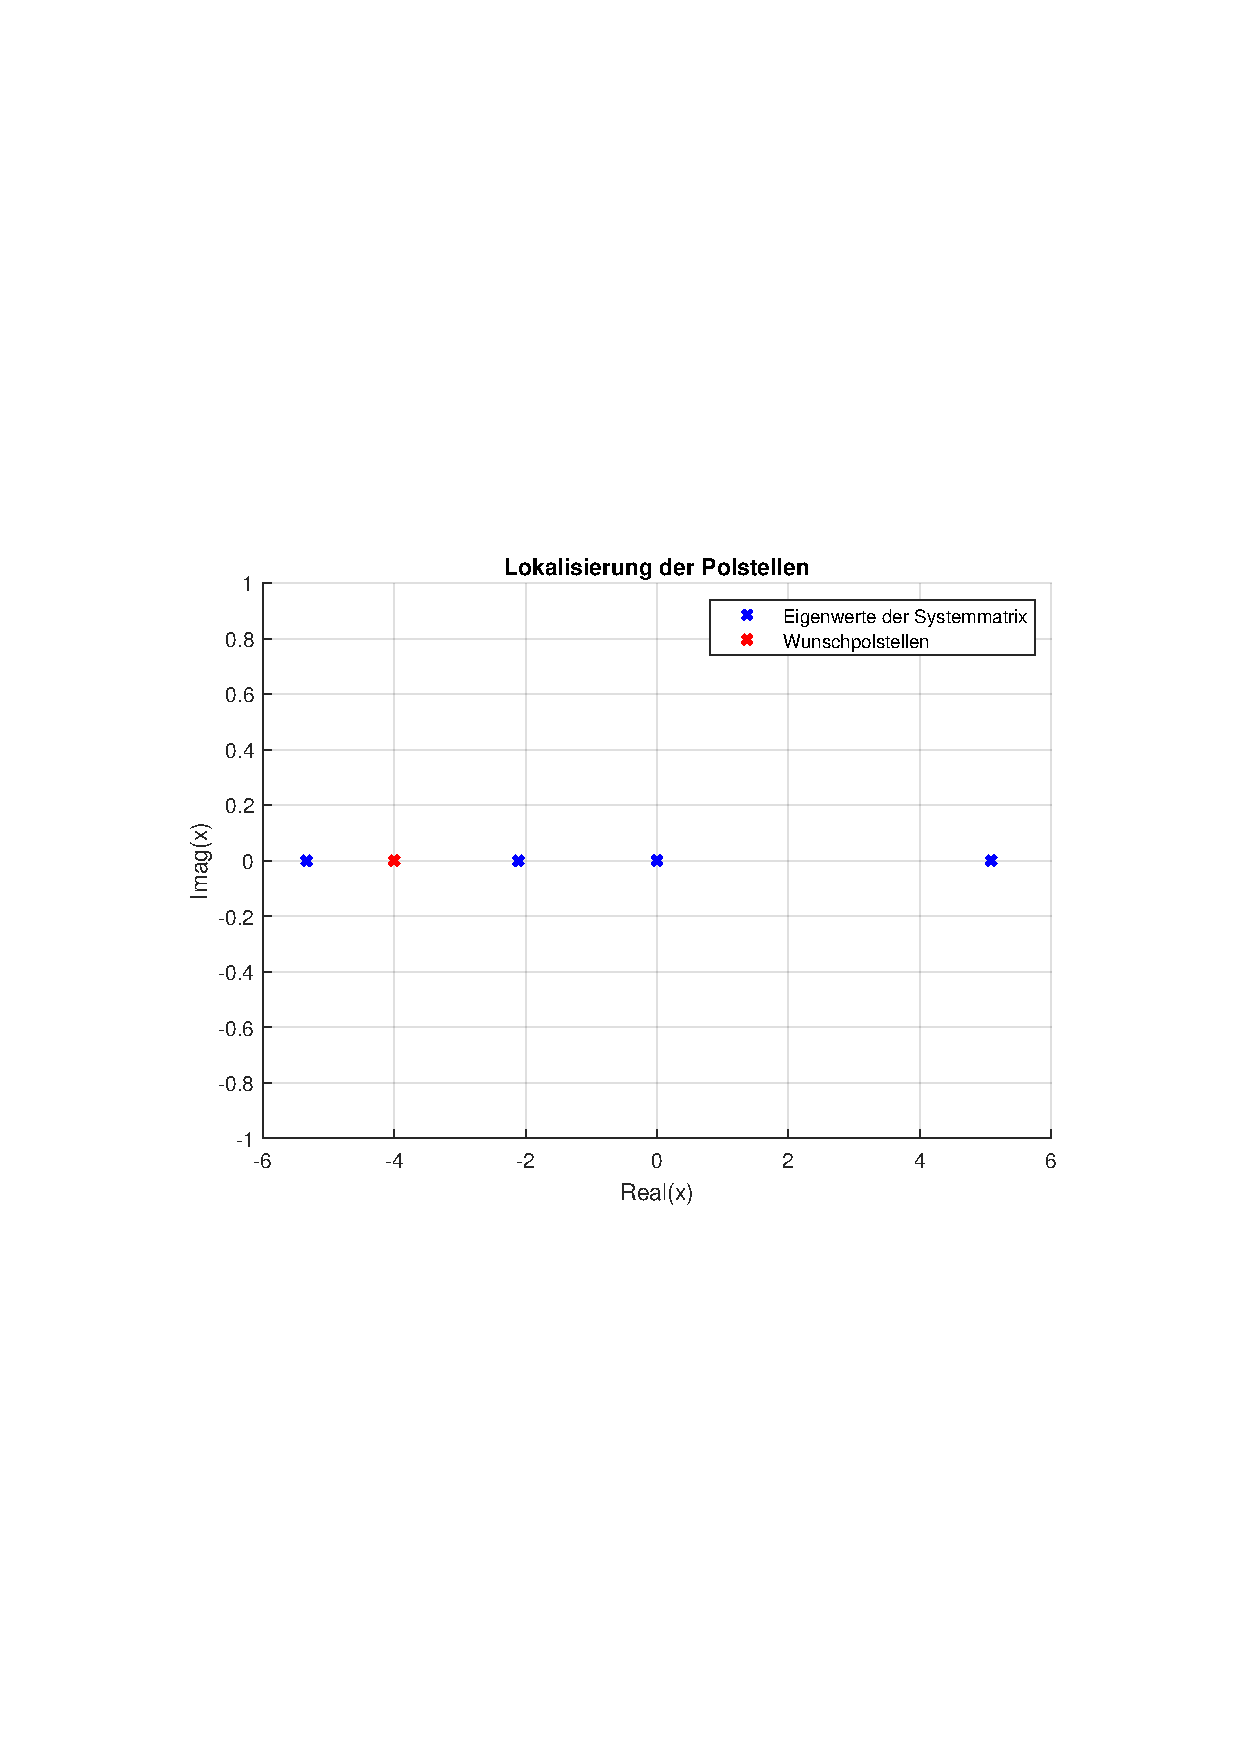
\includegraphics[width=0.75\textwidth]{Bilder/Polstellen_Ackermann.pdf}}
    \caption[Polstellenlage einfacher Zustandsregler]{Polstellenlagen des Systems mit einfachen Zustandsregler}
    \label{fig:Bild8}
\end{figure}

Zur Bestimmung der Koeffizienten $\alpha_{\mathrm{n}}$ bis $\alpha_{\mathrm{0}}$ des geregelten Systems, wird das charakteristische Polynom ausmultipliziert und die Wunschpolstellen eingesetzt.\\\\
Berechnung der Koeffizienten:

\begin{align*}
    \underline{P}(s) &= (s-s_{\mathrm{P1}})\cdot(s-s_{\mathrm{P2}})\cdot(s-s_{\mathrm{P3}})\cdot(s-s_{\mathrm{P4}}) \\
    \underline{P}(s) &= s^4-s^3\cdot(s_{\mathrm{P1}}+s_{\mathrm{P2}}+s_{\mathrm{P3}}+s_{\mathrm{P4}}) \nonumber \\ 
    &\quad +s^2\cdot(s_{\mathrm{P1}}\cdot(s_{\mathrm{P2}}+s_{\mathrm{P3}}+s_{\mathrm{P4}})+s_{\mathrm{P2}}\cdot(s_{\mathrm{P3}}+s_{\mathrm{P4}})+s_{\mathrm{P3}}\cdot s_{\mathrm{P4}}) \nonumber \\
    &\quad -s\cdot(s_{\mathrm{P1}}\cdot(s_{\mathrm{P2}}\cdot s_{\mathrm{P3}}+s_{\mathrm{P2}}\cdot s_{\mathrm{P4}}+s_{\mathrm{P3}}\cdot s_{\mathrm{P4}})+s_{\mathrm{P2}}\cdot s_{\mathrm{P3}}\cdot s_{\mathrm{P4}}) \nonumber \\
    &\quad +(s_{\mathrm{P1}}\cdot s_{\mathrm{P2}}\cdot s_{\mathrm{P3}}\cdot s_{\mathrm{P4}})
\end{align*}
\newline
Das charakteristische Polynom und die Koeffizienten folgen zu:

\begin{align}
    \underline{P}(s) &= s^4+16\cdot s^3+96\cdot s^2+256\cdot s+256 \nonumber \\
    \underline{\alpha} &=
    \begin{bmatrix}
        256 & 256 & 96 & 16 & 1
    \end{bmatrix} \label{eq:Gleichung38}
\end{align}
\newline
Zur Berechnung der Verstärkungsfaktoren des Reglers wird die letzte Zeile $t_{\mathrm{n}}^T$ der inversen Steuerbarkeitsmatrix $Q_{\mathrm{s}}^{-1}$ benötigt. Diese berechnet sich zu:

\begin{align*}
    \underline{Q}_{\mathrm{s}}^{-1} &=
    \begin{bmatrix}
         0 & -0.8333 & 1.9651 & -26.7984 \\
        -0.8333 & 1.9651 & -26.7984 & 67.7740 \\
        0 & 0.3333 & -0.7784 & 2.5264 \\
        0.3333 & -0.7784 & 2.5264 & -7.5869
    \end{bmatrix}^{-1} \\
    \underline{Q}_{\mathrm{s}}^{-1} &=
    \begin{bmatrix}
        0 & -0.1040 & 7 & 3.26 \\
        -0.1092 & -0.1142 & 3.2665 & 0.2854 \\
        -0.1165 & -0.0488 & 0.2885 & 0.1221 \\
        -0.0489 & 0 & 0.1223 & -0.0001
    \end{bmatrix}
\end{align*}
\newline
Die letzte Zeile der inversen Matrix ist:

\begin{align} \label{eq:Gleichung39}
    \underline{t}_{\mathrm{4}}^T &=
    \begin{bmatrix}
        -0.0489 & 0 & -0.1223 & -0.0001
    \end{bmatrix}
\end{align}
\newline
Die finale Berechnung erfolgt auf Grundlage der \autoref{eq:Gleichung40}. Durch das Einsetzen der letzten Zeile der inversen Steuerbarkeitsmatrix (\autoref{eq:Gleichung39}), der Faktoren aus \autoref{eq:Gleichung38} und der Systemmatrix A folgt für die \textbf{Verstärkungsfaktoren} $\underline{k}^T_{\mathrm{Acker}}$ der Zustandsrückführung:

\begin{empheq}[box=\widefbox]{align}
    \underline{k}^T &= \underline{t}_{\mathrm{n}}^T\cdot(\alpha_{\mathrm{0}}\cdot\underline{I} + \alpha_{\mathrm{1}}\cdot \underline{A} + ... + \alpha_{\mathrm{n-1}}\cdot \underline{A}^{n-1}+\underline{A}^n) \label{eq:Gleichung40}\\
    \underline{k}^T_{\mathrm{Acker}} &=
    \begin{bmatrix}
        -159.9929 & -31.7079 & -31.3150 & -38.3441
    \end{bmatrix} \label{eq:Gleichung41}
\end{empheq}

\subsection{Vorsteuerung}

Mithilfe des Vorfilters können Referenzpositionen für die Systemzustände vorgegeben werden. Im weiteren Verlauf wird lediglich eine Referenzposition des Wagens vorgegeben, d.h. der Wagen fährt während des Pendelschwingens eine Endlage abweichend zum Ursprung an. Der Referenzwert wird auf den Systemeingang gegeben. Dieser wird anschließend mit dem Vorfilter $\underline{F}$ multipliziert. Weiterhin erfolgt die Verrechnung mit den Faktoren $\underline{k}$, welche analog zum \autoref{sec:Ackermann-Formel} berechnet werden (\autoref{fig:Bild9}). Die \textbf{Eingangsgleichung des Systems} ist gegeben durch:

\begin{align}\label{eq:Gleichung42}
    \underline{u}(t) &= -\underline{k}\cdot\underline{x}(t)+\underline{F}\cdot\underline{y}_{ref}(t)
\end{align}

\begin{figure}[H]
    \centering
    \fbox{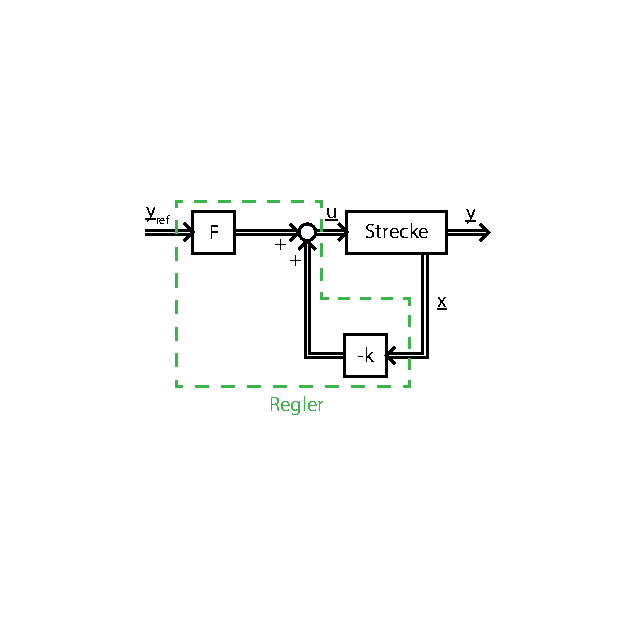
\includegraphics[width=0.5\textwidth]{Bilder/Vorsteuerung.pdf}}
    \caption[Reglerstruktur Vorsteuerung]{Schematische Darstellung der Reglerstruktur der Referenzwert-Vorsteuerung}
    \label{fig:Bild9}
\end{figure}

Zur Ermittlung der Matrix $\underline{F}$ des Vorfilters werden zuerst die im Zeitbereich geltenden Kriterien aufgestellt. Der Ausgang des Systems $\underline{y}(t)$ muss für $t \to \infty$ in den Referenzwert $\underline{y}_{ref}$ laufen. Der Referenzwert wird als konstant angenommen. Dazu gelten folgende \textbf{Kriterien im Zeitbereich}:
\begin{align}
    \lim_{t \to \infty} \underline{y}(t) &= \underline{y}_{ref} = \underline{y}_{0ref} = const. \label{eq:Gleichung43}\\
    \underline{y}_{ref}(t) &=
    \begin{cases}
        \underline{y}_{0ref} & t \geq 0 \\
        0 & \, \text{sonst}
    \end{cases} \label{eq:Gleichung44}
\end{align}
\newline
Da die Berechnungen im Zeitbereich aufwendig sind, werden weitere Betrachtungen im Laplace-Bereich vorgenommen. Vorteil der Transformation ist das Rechnen mit algebraischen Gleichungen. Zur Überführung des Ansatzes aus \autoref{eq:Gleichung43} wird der \textbf{Grenzwertsatz der Laplace-Transformation} angewandt. Das Referenzzeitsignal $\underline{y}_{ref}(t)$ aus \autoref{eq:Gleichung44} wird ebenfalls überführt.

\begin{align}
    \lim_{t \to \infty} \underline{y}(t) &= \lim_{s \to 0} s\cdot\underline{Y}(s) = \underline{y}_{ref} = \underline{y}_{0ref} \label{eq:Gleichung45}\\
    \underline{Y}_{ref}(s) &= \frac{1}{s}\cdot\underline{y}_{0ref} \label{eq:Gleichung46}
\end{align}
\newline
Für weitere Betrachtungen wird das Zustandsraummodell der Strecke in den Laplace-Bereich transformiert:

\begin{align}
    \underline{\dot{x}}(t) &= \underline{A}\cdot\underline{x}+\underline{B}\cdot\underline{u}(t)\quad\laplace\quad s\cdot \underline{X}(s) = \underline{A}\cdot\underline{X}(s)+\underline{B}\cdot\underline{U}(s) \label{eq:Gleichung47}\\
    \underline{y}(t) &= \underline{C}\cdot\underline{x}(t) \quad\laplace\quad \underline{Y}(s) = \underline{C}\cdot\underline{X}(s) \label{eq:Gleichung48}
\end{align}
\newline
Die \autoref{eq:Gleichung47} wird nach $\underline{X}(s)$ umgestellt und entsprechend in die Laplace-transformierte Ausgangsgleichung $\underline{Y}(s)$ eingesetzt. Aus der Umstellung geht hervor, dass das System durch eine Multiplikation aus einer Übertragungsfunktion $\underline{G}(s)$ und dem Eingangssignal $\underline{U}(s)$ gebildet werden kann.

\begin{align}
    \underline{B}\cdot\underline{U}(s) &= (s\cdot\underline{I}-\underline{A})\cdot\underline{X}(s) \label{eq:Gleichung49}\\
    \underline{X}(s) &= (s\cdot\underline{I}-\underline{A})^{-1}\cdot\underline{B}\cdot\underline{U}(s) \nonumber \\
    \underline{Y}(s) &= \underline{C}\cdot(s\cdot\underline{I}-\underline{A})^{-1}\cdot\underline{B}\cdot\underline{U}(s) \label{eq:Gleichung50}\\
    \underline{G}(s) &= \underline{C}\cdot(s\cdot\underline{I}-\underline{A})^{-1}\cdot\underline{B} \nonumber
\end{align}
\newline
Die Eingangsgleichung des Systems (\autoref{eq:Gleichung42}) wird transformiert und anschließend in \autoref{eq:Gleichung49} eingesetzt.

\begin{align*}
    \underline{U}(s) &= -\underline{k}\cdot\underline{X}(s)+\underline{F}\cdot\underline{Y}_{\mathrm{ref}}(s)
\end{align*}
\newline
Einsetzen und Umformung nach $\underline{X}(s)$:

\begin{align}
    \underline{B}\cdot(\underline{F}\cdot\underline{Y}_{\mathrm{ref}}(s)-\underline{k}\cdot\underline{X}(s)) &= (s\cdot\underline{I}-\underline{A})\cdot\underline{X}(s) \nonumber \\
    \underline{B}\cdot \underline{F}\cdot\underline{Y}_{\mathrm{ref}}(s) &= (s\cdot\underline{I}-\underline{A}+\underline{B}\cdot{\underline{k}})\cdot\underline{X}(s) \nonumber \\
    \underline{X}(s) &= (s\cdot\underline{I}-\underline{A}+\underline{B}\cdot{\underline{k}})^{-1}\cdot\underline{B}\cdot \underline{F}\cdot\underline{Y}_{\mathrm{ref}}(s) \label{eq:Gleichung51}
\end{align}
\newline
Die \autoref{eq:Gleichung51} wird in \autoref{eq:Gleichung48} eingesetzt, um die \textbf{Übertragungsfunktion des geschlossenen Regelkreises} zu erhalten.

\begin{align}
        \underline{Y}(s) &= \underline{C}\cdot(s\cdot\underline{I}-\underline{A}+\underline{B}\cdot{\underline{k}})^{-1}\cdot\underline{B}\cdot F\cdot\underline{Y}_{\mathrm{ref}}(s) \label{eq:Gleichung52}
\end{align}
\newline
Aus der vorangegangenen Betrachtung ist nur die Matrix $\underline{F}$ des Vorfilters unbekannt. Um dasjenige $F$ zu ermitteln, welches die \textbf{stationäre Exaktheit} erfüllt, wird der Grenzwertsatz aus \autoref{eq:Gleichung45} angesetzt und die Übertragungsfunktion des geschlossenen Regelkreises (\autoref{eq:Gleichung52}) eingesetzt.

\begin{align}
    \lim_{s \to 0} s\cdot \underline{Y}(s) &= \underline{y}_{0ref} \nonumber \\
    \lim_{s \to 0} s\cdot (\underline{C}\cdot(s\cdot\underline{I}-\underline{A}+\underline{B}\cdot{\underline{k}})^{-1}\cdot\underline{B}\cdot\underline{F}\cdot\frac{1}{s}\cdot\underline{y}_{0ref}) &= \underline{y}_{0ref} \label{eq:Gleichung53}
\end{align}
\newline
Nach dem Vereinfachen der \autoref{eq:Gleichung53} geht hervor, dass der Term $\underline{C}\cdot(-\underline{A}+\underline{B}\cdot{\underline{k}})^{-1}\cdot\underline{B}\cdot\underline{F}$ der Einheitsmatrix $\underline{I}$ gleichen muss (\autoref{eq:Gleichung54}). Andernfalls ist die Gleichung nicht erfüllbar. Durch die Kenntnis kann die \textbf{Matrix $\underline{F}$ des Vorfilters} bestimmt werden durch:

\begin{empheq}[box=\widefbox]{align}
    \underline{C}\cdot(-\underline{A}+\underline{B}\cdot{\underline{k}})^{-1}\cdot\underline{B}\cdot\underline{F} &= \underline{I} \label{eq:Gleichung54}\\
    \underline{F} = (\underline{C}\cdot(-\underline{A}+\underline{B}\cdot{\underline{k}})^{-1}\cdot\underline{B})^{-1} \label{eq:Gleichung55}
\end{empheq}
\newline
Die Anwendbarkeit des Reglergesetztes ist eingeschränkt, da nur quadratische Matrizen invertierbar sind. Die Dimensionen der einzelnen Matrizen lauten wie folgt:

\begin{itemize}
    \item $A\in\mathbb{R}^{(nxn)}$
    \item $B\in\mathbb{R}^{(nxm)}$
    \item $C\in\mathbb{R}^{(pxn)}$
    \item $k\in\mathbb{R}^{(mxn)}$
\end{itemize}

Die Matrix $\underline{F}$ ist quadratisch, sobald $p = m$ gilt, d.h. die Anzahl der Systemeingänge muss gleich der Anzahl der Systemausgänge sein, d.h. die benötigte \textbf{C-Matrix zur Berechnung des Vorfilters} lautet:

\begin{align*}
   C = [0\quad 0\quad 1\quad 0]. 
\end{align*}
\newline
Die \textbf{Polstellen} der Reglerstuktur werden folgendermaßen festgelegt:

\begin{empheq}[box=\widefbox]{align} \label{eq:Gleichung56}
    \underline{s}_{P} &=
    \begin{bmatrix}
        -4.5 & -4.5 & -4.5 & -4.5
    \end{bmatrix}
\end{empheq}
\newline
Die Polstellenlagen sind in \autoref{fig:Bild10} dargestellt.

\begin{figure}[H]
    \centering
    \fbox{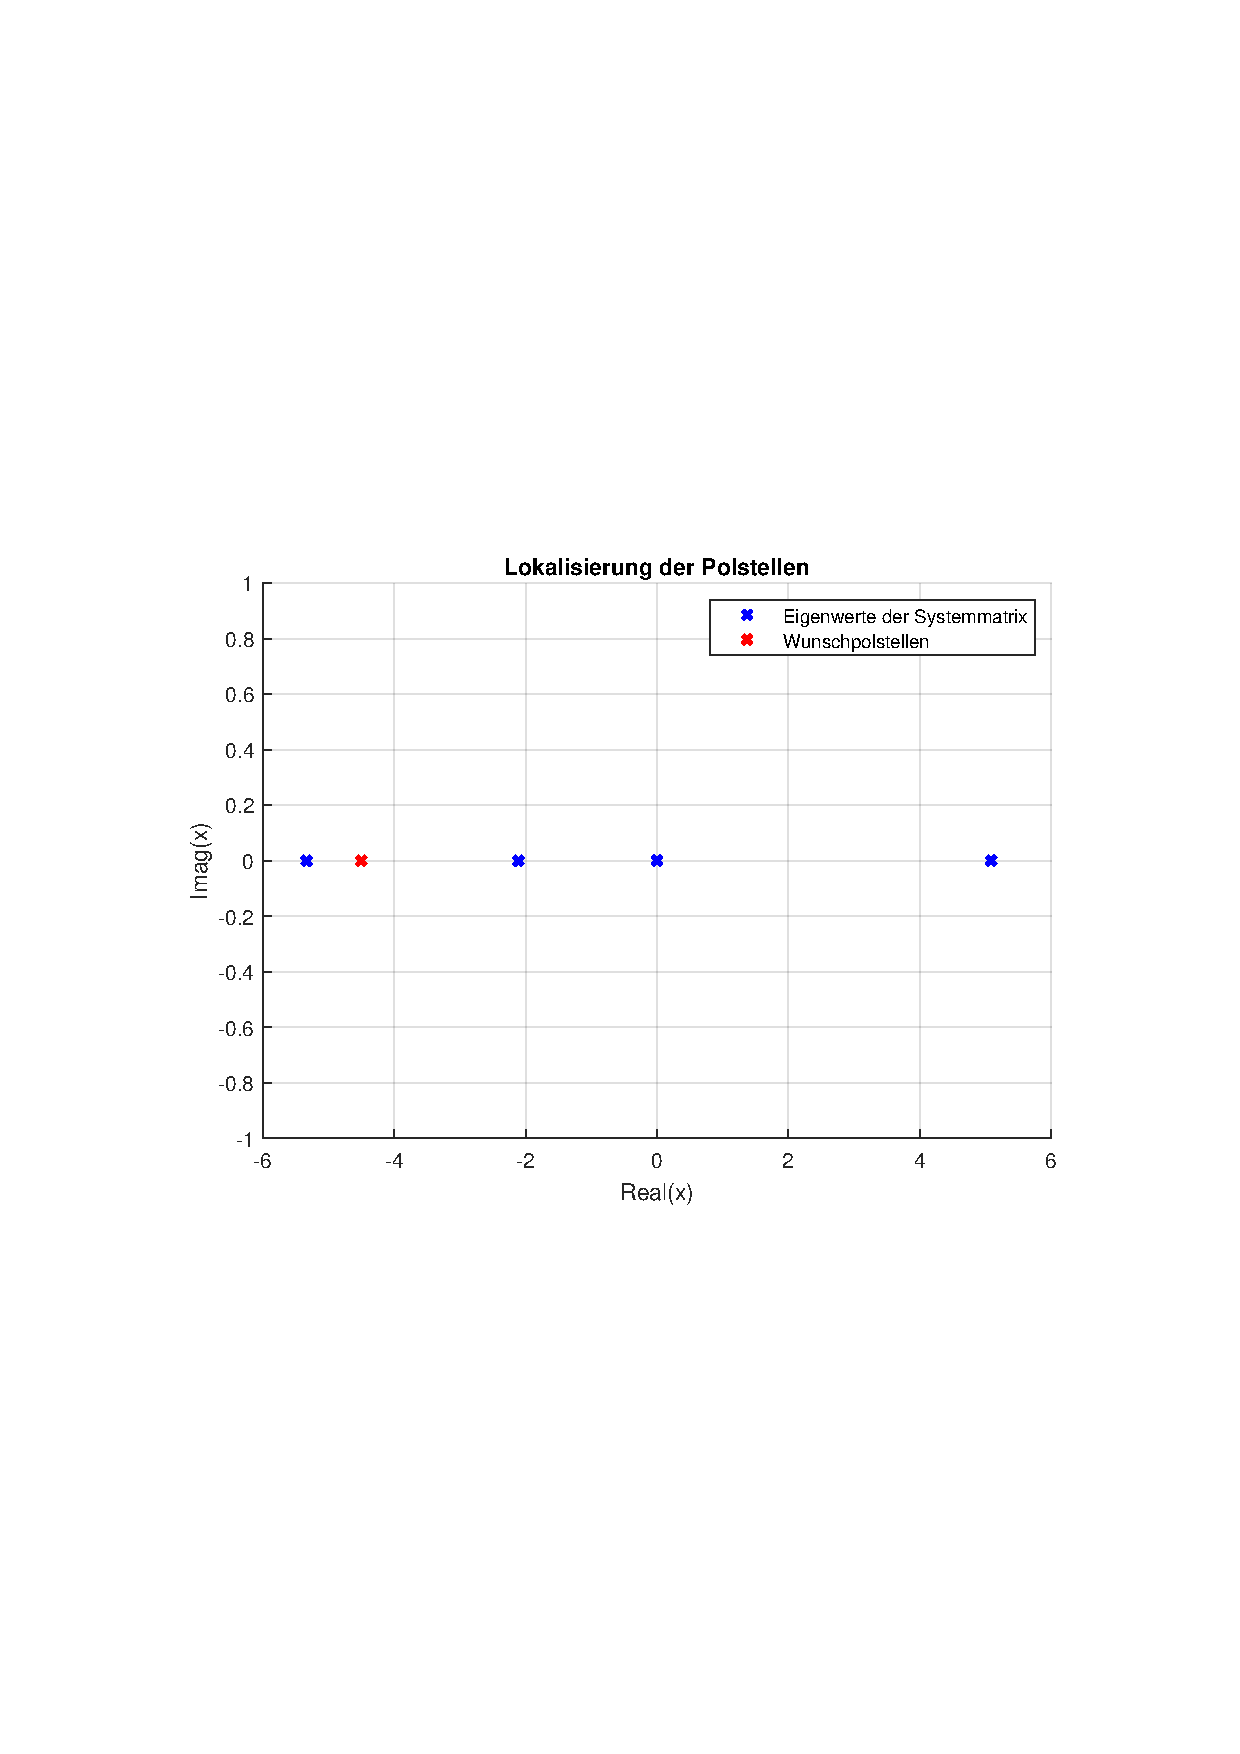
\includegraphics[width=0.75\textwidth]{Bilder/Polstellen_Vorsteuerung.pdf}}
    \caption[Polstellenlage Vorsteuerung]{Polstellenlagen des Systems mit Referenzwert-Vorsteuerung}
    \label{fig:Bild10}
\end{figure}

 Die \textbf{k-Faktoren der Zustandsrückführung} folgen zu:
 
\begin{empheq}[box=\widefbox]{align} \label{eq:Gleichung57}
    \underline{k}^T_{Vor} &=
    \begin{bmatrix}
        -198.2525 & -39.4238 & -50.1606 & -51.6339
    \end{bmatrix}
\end{empheq}
\newline
Wird das linearisierte Zustandsraummodell (\autoref{eq:Gleichung33}) und die Faktoren $\underline{k}$ aus \autoref{eq:Gleichung57} in das Reglergesetz eingesetzt, resultiert der \textbf{Faktor $F$} zu

\begin{equation} \label{eq:Gleichung58}
    \boxed{F = -50.1606}.
\end{equation}
\newline
Der Faktor $F$ ist ein skalarer Wert, da nur ein Referenzwert vorliegt.

\subsection{I-Regelung} \label{sec:iregler}
Bei der Regelung mit Referenzwert-Vorsteuerung entsteht ein Regelfehler, welcher zu einem ungenauen Ergebnis führt. Der Regelfehler folgt aus der Differenz des Referenzwertes am Systemeingang ($\underline{y}_{\mathrm{ref}}$) und dem zugehörigen Endwert am Systemausgang ($\underline{y}$). Um den Regelfehler zu minimieren, wird dieser entsprechend aufintegriert. Die Folge ist ein größerer Stellgrößenaufwand. Die Systemstruktur ist in \autoref{fig:Bild11} dargestellt. Das Reglergesetzt mit den Faktoren $\underline{k}_{\mathrm{I}}$ (I-Verstärkungskoeffizient) und $\underline{k}_{\mathrm{x}}$ (Zustandsrückführungskoeffizient) kann in \autoref{eq:Gleichung59} nachvollzogen werden.

\begin{align}\label{eq:Gleichung59}
    \underline{u} &= \underline{k}_{\mathrm{I}}\cdot\int_{0}^t(\underline{y}_{\mathrm{ref}}-\underline{y})d\tau-\underline{k}_{\mathrm{x}}\cdot\underline{x}
\end{align}

\begin{figure}[H]
    \centering
    \fbox{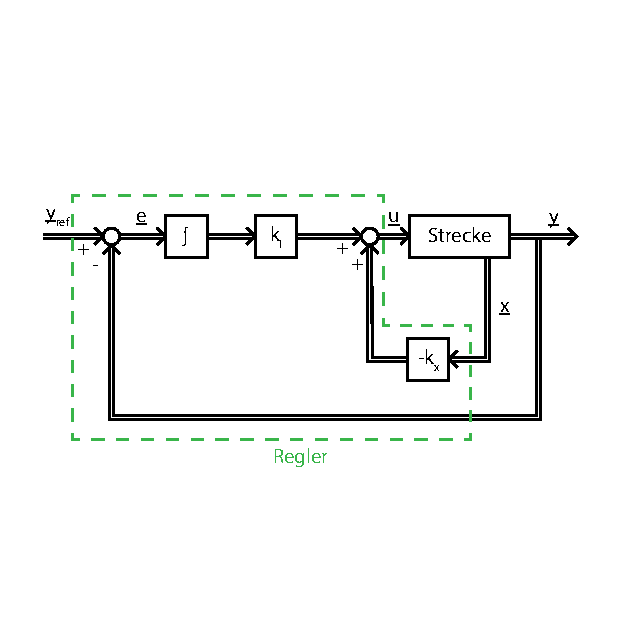
\includegraphics[width=0.7\textwidth]{Bilder/I-Regler.pdf}}
    \caption[Reglerstruktur I-Regelung]{Schematische Darstellung der Reglerstruktur mit I-Regelung}
    \label{fig:Bild11}
\end{figure}

Mit der Definition (\autoref{eq:Gleichung60}) wird das Reglergesetz verändert aufgeschrieben. Aus der Definition

\begin{align}\label{eq:Gleichung60}
    \underline{x}_{\mathrm{I}}& :=\int_{0}^t(\underline{y}_{\mathrm{ref}}-\underline{y})d\tau
\end{align}
\newline
folgt nach Einsetzen und Umformen

\begin{align}
    \underline{u} &= \underline{k}_{\mathrm{I}}\cdot\underline{x}_{\mathrm{I}}-\underline{k}_{\mathrm{x}}\cdot\underline{x} \nonumber \\
    \underline{u} &= -\underline{k}_{\mathrm{x}}\cdot\underline{x}+\underline{k}_{\mathrm{I}}\cdot\underline{x}_{\mathrm{I}} \nonumber\\
    \underline{u} &= -
    \begin{bmatrix}
        \underline{k}_{\mathrm{x}} & -\underline{k}_{\mathrm{I}}
    \end{bmatrix}
    \cdot
    \begin{bmatrix}
        \underline{x} \\
        \underline{x}_{\mathrm{I}}
    \end{bmatrix} \label{eq:Gleichung61} \\
    \underline{\tilde{k}} &= 
    \begin{bmatrix}
        \underline{k}_{\mathrm{x}} & -\underline{k}_{\mathrm{I}}
    \end{bmatrix}. \label{eq:Gleichung62}
\end{align}
\newline
Um das erweiterte Zustandsraummodell aufstellen zu können, wird der \textbf{Zustandsänderungsvektor} $\underline{\dot{\tilde{x}}}$ definiert.

\begin{align}
    \underline{\tilde{x}} &=
    \begin{bmatrix}
        \underline{x} \\
        \underline{x}_{\mathrm{I}}
    \end{bmatrix} \nonumber \\
    \underline{\dot{\tilde{x}}} &= 
    \begin{bmatrix}
        \underline{\dot{x}} \\
        \underline{\dot{x}}_{\mathrm{I}}
    \end{bmatrix} \label{eq:Gleichung63}
\end{align}
\newline
Die benötigen Vektoren folgen zu:

\begin{align}
    \underline{\dot{x}} &= \underline{A}\cdot\underline{x}+\underline{B}\cdot\underline{u} \label{eq:Gleichung64}\\
    \underline{\dot{x}}_{\mathrm{I}} &= \frac{d}{dx}\cdot\int_{0}^t(\underline{y}_{\mathrm{ref}}-\underline{y})d\tau = \underline{y}_{\mathrm{ref}}-\underline{y} \nonumber \\
    \underline{\dot{x}}_{\mathrm{I}} &= \underline{y}_{\mathrm{ref}}-\underline{C}\cdot\underline{x} \label{eq:Gleichung65}
\end{align}
\newline
Auf Grundlage der \autoref{eq:Gleichung63} bis \autoref{eq:Gleichung65} folgt das \textbf{erweiterte Zustandsraummodell} zu

\begin{empheq}[box=\widefbox]{align} \label{eq:Gleichung66}
    \underline{\dot{\tilde{x}}} &= 
    \begin{bmatrix}
        \underline{A} & \underline{0} \\
        -\underline{C} & \underline{0}
    \end{bmatrix} \cdot \underline{\tilde{x}} +
    \begin{bmatrix}
        \underline{B} \\
        \underline{0}
    \end{bmatrix} \cdot\underline{u} +
    \begin{bmatrix}
        \underline{0} \\
        \underline{I}
    \end{bmatrix} \cdot\underline{y}_{ref}
\end{empheq}
\newline
mit

\begin{align*}
    \underline{\tilde{A}} &= 
    \begin{bmatrix}
        \underline{A} & \underline{0} \\
        -\underline{C} & \underline{0}
    \end{bmatrix} \quad ; \underline{\tilde{A}}\in\mathbb{R}^{(n+p)x(n+p)}\\
    \underline{\tilde{B}} &= 
    \begin{bmatrix}
        \underline{B} \\
        \underline{0}
    \end{bmatrix}\qquad ; \underline{\tilde{B}}\in\mathbb{R}^{(n+p)x(m)}\\
    \underline{\tilde{B}}_{\mathrm{y}} &= 
    \begin{bmatrix}
        \underline{0} \\
        \underline{I}
    \end{bmatrix}\qquad  ;\underline{\tilde{B}}_{\mathrm{y}}\in\mathbb{R}^{(n+p)x(p)}.
\end{align*}
\newline
Die Matrix C wird analog zum Regler mit Referenzwert-Vorsteuerung betrachtet. Mithilfe der Matrizen $\underline{\tilde{A}}$ und $\underline{\tilde{B}}$ werden die Verstärkungskoeffizienten ($\underline{k}_{\mathrm{x}}$ und $\underline{k}_{\mathrm{I}}$) analog zu \autoref{sec:Ackermann-Formel} berechnet. Die \textbf{Polstellen des Reglers} werden entsprechend festgelegt (\autoref{eq:Gleichung67}).

\begin{empheq}[box=\widefbox]{align} \label{eq:Gleichung67}
    \underline{s}_{\mathrm{P}} &= 
    \begin{bmatrix}
        -3.2 & -3.2 & -3.2 & -3.2 & -3.2
    \end{bmatrix}
\end{empheq}
\newline
Die Länge des Vektors folgt auf Grundlage der Größe der Matrix $\underline{\tilde{A}}$. Die Lage der Polstellen ist in \autoref{fig:Bild12} dargestellt.

\begin{figure}[H]
    \centering
    \fbox{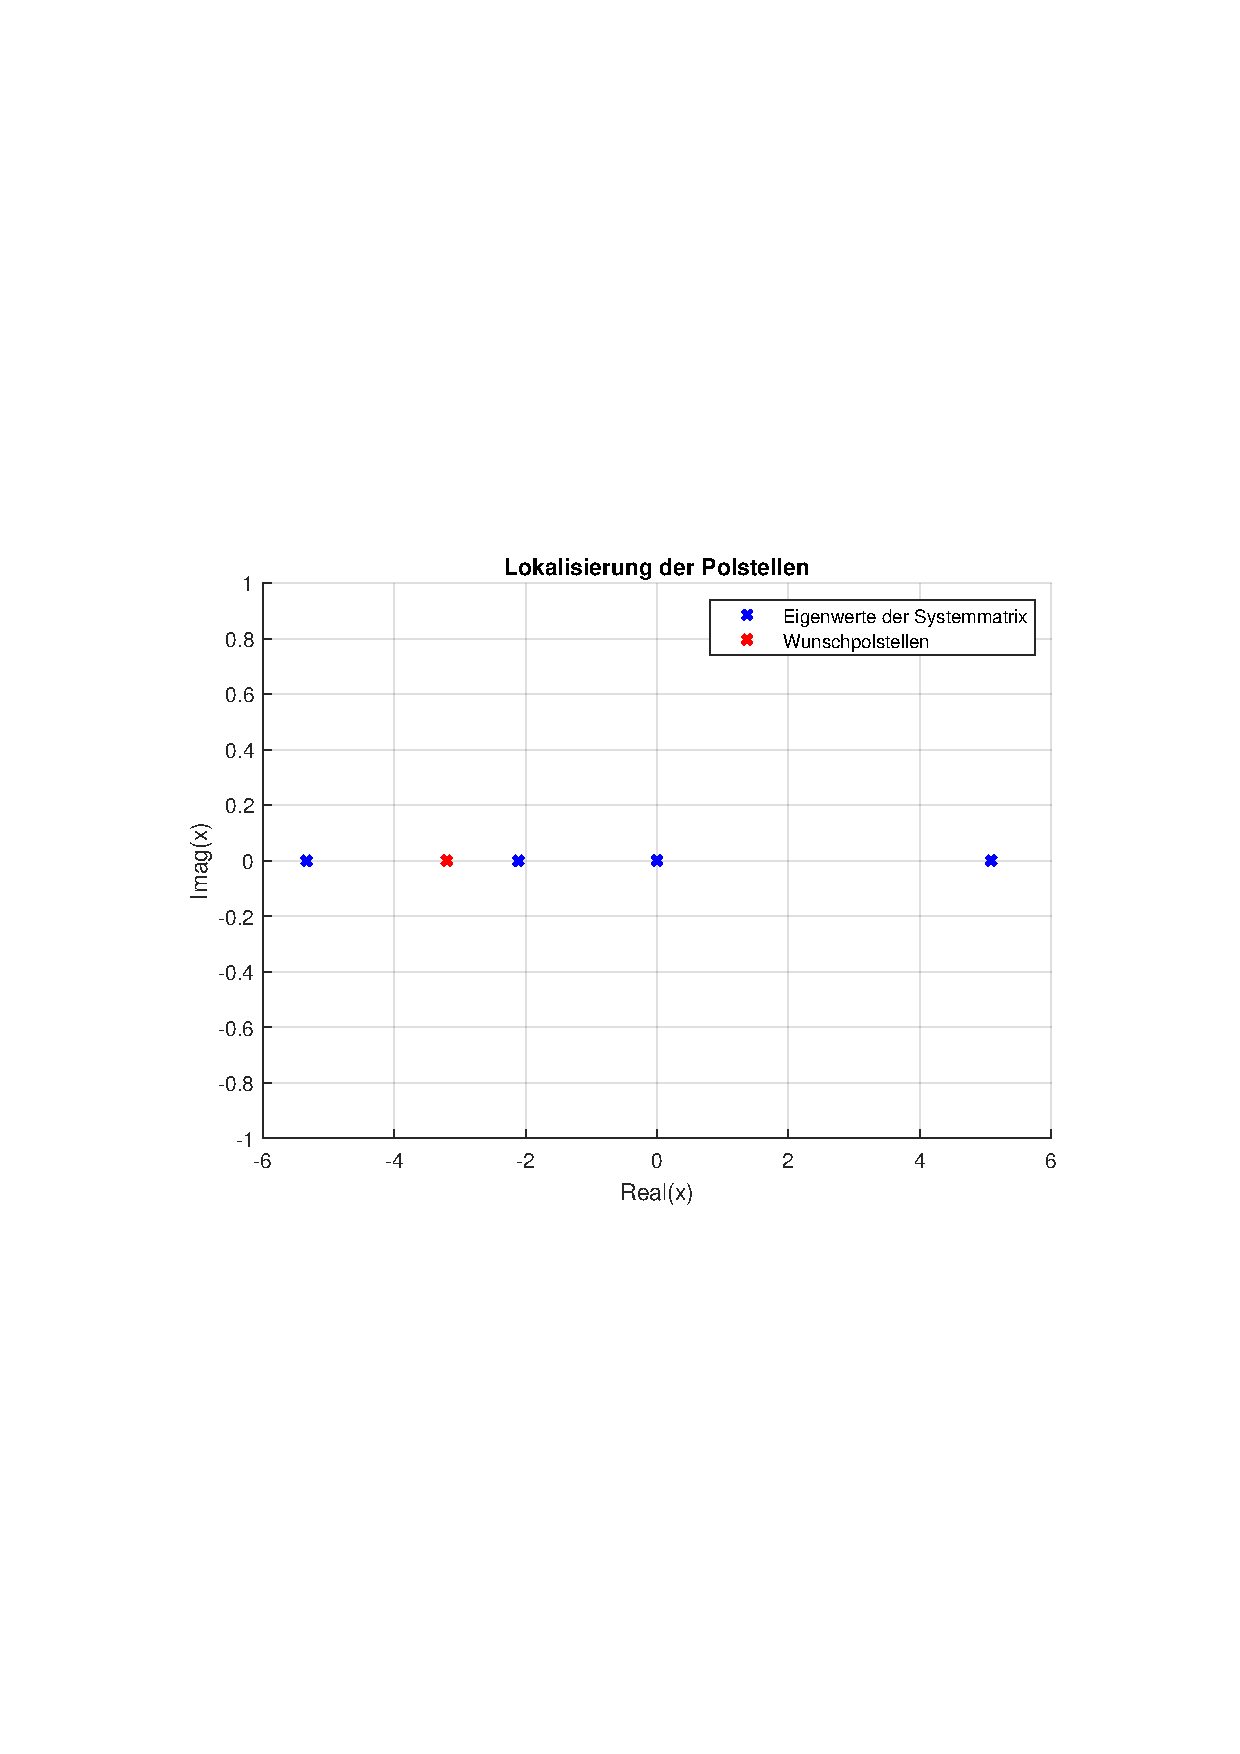
\includegraphics[width=0.75\textwidth]{Bilder/Polstellen_I_Regelung.pdf}}
    \caption[Polstellenlage I-Regelung]{Polstellenlage des Systems mit I-Regelung}
    \label{fig:Bild12}
\end{figure}

Die \textbf{$\underline{\tilde{k}}$-Matrix} resultiert zu:

\begin{align} \label{eq:Gleichung68}
    \underline{\tilde{k}} &= 
    \begin{bmatrix}
        -180.9111 & -35.8968 & -64.1713 & -48.8165 & 41.0452
    \end{bmatrix}
\end{align}
\newline
Gemäß \autoref{eq:Gleichung62} folgen die Verstärkungskoeffizienten (unterteilt in \textbf{Zustandsrückführungskoeffizienten} und \textbf{I-Verstärkungskoeffizienten}) wie nachfolgend gezeigt:

\begin{empheq}[box=\widefbox]{align} \label{eq:Gleichung69}
    \underline{k}_{\mathrm{x}} &= 
    \begin{bmatrix}
        -180.9111 & -35.8968 & -64.1713 & -48.8165
    \end{bmatrix}
\end{empheq}

\begin{empheq}[box=\widefbox]{align} \label{eq:Gleichung70}
    \underline{k}_{\mathrm{I}} &= [-41.0452]
\end{empheq}

\section{Reglervalidierung} \label{sec:reglervalidierung}

Ziel der Reglervalidierung ist das Bestätigen des Regelverhaltens der modellierten drei Regler aus dem \autoref{sec:Zustandsreglerentwurf}. Dies wird mit Hilfe des Matlab Tools \textit{Simulink} durchgeführt. Die zuvor in Matlab berechneten Matrizen (siehe \zB \autoref{eq:Gleichung41}) werden an das Simulink-Modell übergeben und dort genutzt. Die Simulationsergebnisse werden anschließend auf ihre Plausibilität geprüft. Dazu werden zum einen die Eingangsparameter (Anfangsauslenkung und Referenzposition) variiert und zum anderen wird der jeweilige Regler am linearen als auch am nichtlinearen Modell getestet.

\subsection{Validierung des linearen Modells}

Zunächst findet die Validierung der Regler am linearen Zustandsraummodell der Strecke statt. Die Simulink Implementierung der linearen Regelstrecke ist in \autoref{fig:Bild3} dargestellt.

\subsubsection{Zustandsregler mit einfacher Rückführung} \label{sec:val-acker}

Der erste Regler ist erneut der einfache Zustandsregler mit Rückführung. Dessen Implementierung in Simulink kann in \autoref{fig:Bild13} nachvollzogen werden. Als Simulationsergebnisse werden zum einen der Winkel des Pendels $\varphi$, die Wagenposition $x_{\mathrm{M}}$ und die benötigte Eingangskraft $u$ \bzw $F_{\mathrm{a}}$ in Diagrammform dargestellt. \\
Um das Verhalten des Reglers zu testen, wird die Simulation für verschiedene Anfangsauslenkungen des Pendels simuliert. Es wird untersucht, für welche Polstellen des Reglers welche Anfangsauslenkungen maximal eingeprägt werden dürfen, dass die Grenzen der Anlage nicht überschritten werden. Ziel ist es, zu bestätigen, welche Störung des Pendels (Abweichung des Winkels von der oberen Ruhelage) maximal auf dieses einwirken darf, so dass weder die maximale Eingangskraft von 80 N noch die maximale Wagenposition von $\pm$1 m überschritten wird. Dabei gilt es, die Polstellen nicht zu weit nach links auf der Real-Achse zu schieben, da dies den Regler beschleunigen würde. Dies führt jedoch zu größeren wirkenden Kräften und Momenten.

\begin{figure}[H]
    \centering
    \fbox{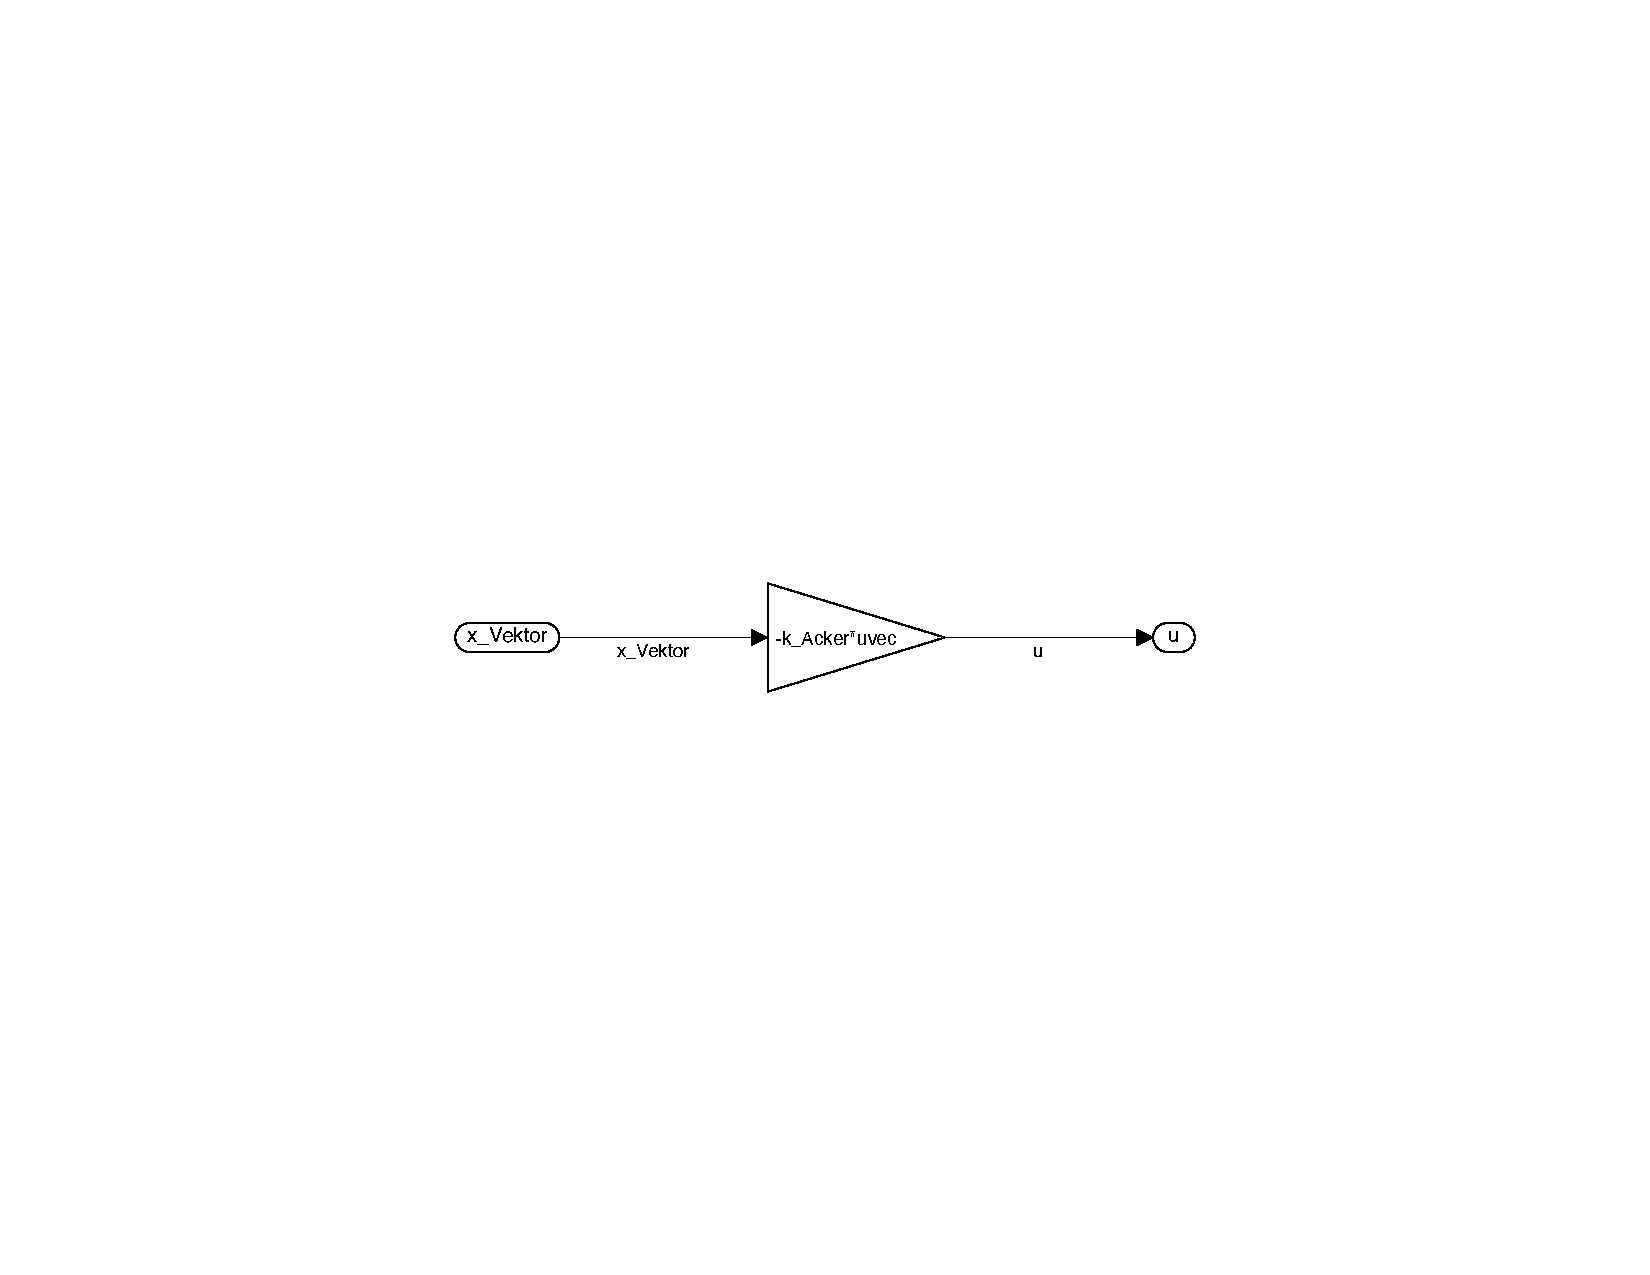
\includegraphics[width=0.7\textwidth]{Bilder/Reglervalidierung/Ackermann_Regler.pdf}}
    \caption[Einfacher Zustandsregler Simulink (linear)]{Simulink Regler-Blockschaltbild für den einfachen Zustandsregler (lineares Zustandsraummodell)}
    \label{fig:Bild13}
\end{figure}

\begin{figure}[H]
    \centering
    \fbox{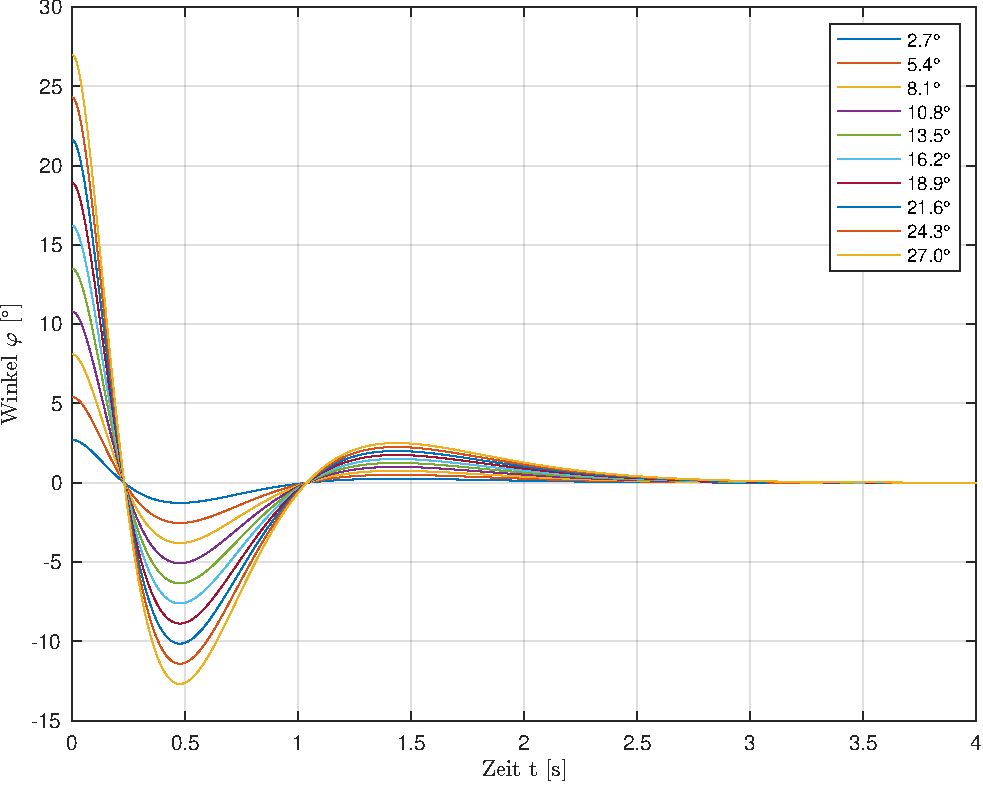
\includegraphics[width=0.64\textwidth]{Bilder/Reglervalidierung/linear_ackermann_phi.pdf}}
    \caption[$\varphi$ für einfachen Zustandsregler (linear)]{$\varphi$ für verschiedene Anfangsauslenkungen am einfachen Zustandsregler für das lineare Zustandsraummodell}
    \label{fig:Bild14}
\end{figure}

\begin{figure}[H]
    \centering
    \fbox{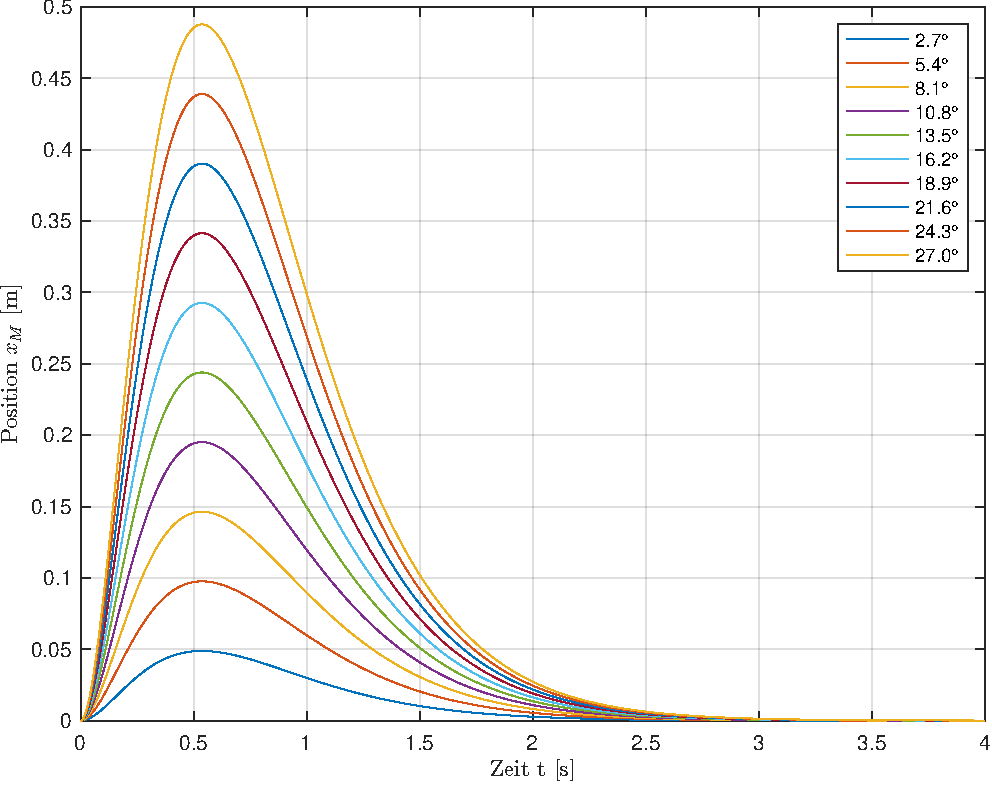
\includegraphics[width=0.64\textwidth]{Bilder/Reglervalidierung/linear_ackermann_xM.pdf}}
    \caption[$x_{\mathrm{M}}$ für einfachen Zustandsregler (linear)]{$x_{\mathrm{M}}$ für verschiedene Anfangsauslenkungen am einfachen Zustandsregler für das lineare Zustandsraummodell}
    \label{fig:Bild15}
\end{figure}

\begin{figure}[H]
    \centering
    \fbox{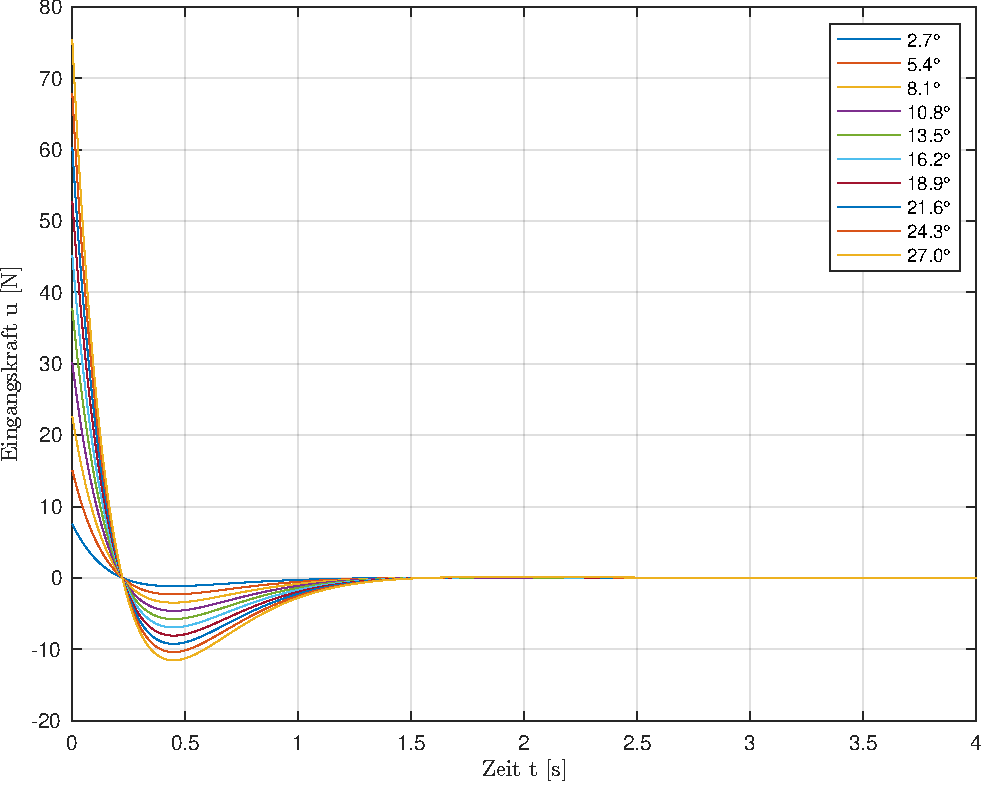
\includegraphics[width=0.64\textwidth]{Bilder/Reglervalidierung/linear_ackermann_u.pdf}}
    \caption[u für einfachen Zustandsregler (linear)]{u für verschiedene Anfangsauslenkungen am einfachen Zustandsregler für das lineare Zustandsraummodell}
    \label{fig:Bild16}
\end{figure}

Die für die oben gezeigten Diagramme gewählten Reglerpolstellen sind in \autoref{eq:Gleichung37} gezeigt. \\
\newline
\autoref{fig:Bild14} bestätigt, dass der Regler wie definiert eine Anfangsauslenkung zu $0^\circ$ (obere Ruhelage) ausregeln kann. Dabei ist zu erkennen, dass der Winkel $\varphi$ des Pendels erst leicht überschwingt, bevor er abschließend ausgeregelt wird. Der gesamte Vorgang dauert \ca 3 s. \\
\newline
Das Verhalten des Wagens ist in \autoref{fig:Bild15} gezeigt. Zu erkennen ist, dass bei einer positiven Anfangsauslenkung eine Bewegung des Wagens nach rechts stattfindet. Die Wagenposition $x_{\mathrm{M}}$ nimmt dementsprechend positive Werte an. Es handelt sich dabei um das zu erwartende Verhalten. Weiterhin bestätigt die Abbildung, dass selbst für einen Auslenkungswinkel von $27^\circ$ die maximale Wagenposition nicht überschritten wird. Von möglichen 100 cm werden lediglich knapp unter 50 cm benötigt. Da der einfache Zustandsregler keine Referenzpositionen für den Wagen entgegennehmen kann, ist die Position dieses am Ende wieder der Nullpunkt. \\
\newline
Das dritte Diagramm (\autoref{fig:Bild16}) zeigt die benötigte Kraft des Motors am Schlitten, um den Wagen in entsprechender Zeit an die zuvor gezeigte Position zu bewegen. Zu erkennen ist, dass für einen Winkel von $27^\circ$ der Motor maximal belastet wird. Es werden \ca 80 N benötigt. Für kleinere Auslenkungen ist weniger Kraft nötig, da auch die Position des Wagens weniger signifikant vom Ausgangspunkt abweicht. Es fällt auf, dass die Initialkraft am größten ist. Dies ist zu erklären über die Beschleunigung des Wagens. Beim Abbremsen kommt es auch hier zu einem Überschwingen, welches durch die negative Beschleunigung zu erwarten ist. Zuletzt ist festzuhalten, dass bereits nach rund 1,5 s der Motor keine Kraft mehr liefern muss. Somit ist die Eingangskraft bereits nach \ca der Hälfte der Ausregelzeit wieder bei u = 0 N  angelangt.\\
\newline
Zusammenfassend kann bestätigt werden, dass sich der Regler erwartungsgemäß verhält und die Grenzen der Anlage bezüglich maximaler Position und Kraft nicht überschritten werden.

\subsubsection{Zustandsregler mit Referenzwert-Vorsteuerung} \label{sec:val-vor}

Nachfolgend soll der Regler mit Vorsteuerung validiert werden. Dessen Simulink-Struktur ist in \autoref{fig:Bild17} aufgezeigt. Im Unterschied zu \autoref{sec:val-acker} kann bei diesem Regler eine Referenzposition für den Wagen vorgegeben werden. \\
In Diagrammform werden erneut der Winkel des Pendels $\varphi$, die Wagenposition $x_{\mathrm{M}}$ und die benötigte Eingangskraft $u$ \bzw $F_{\mathrm{a}}$ dargestellt. Zusätzlich wird die Validierung für verschiedene Referenzpositionen $y_{ref}$ vorgenommen. \\
Ziel ist auch hier das Bestätigen des Einhaltens der Grenzen der Anlage für die gewählten Polstellen bei untersuchten Anfangsauslenkungen und Referenzpositionen. 

\begin{figure}[H]
    \centering
    \fbox{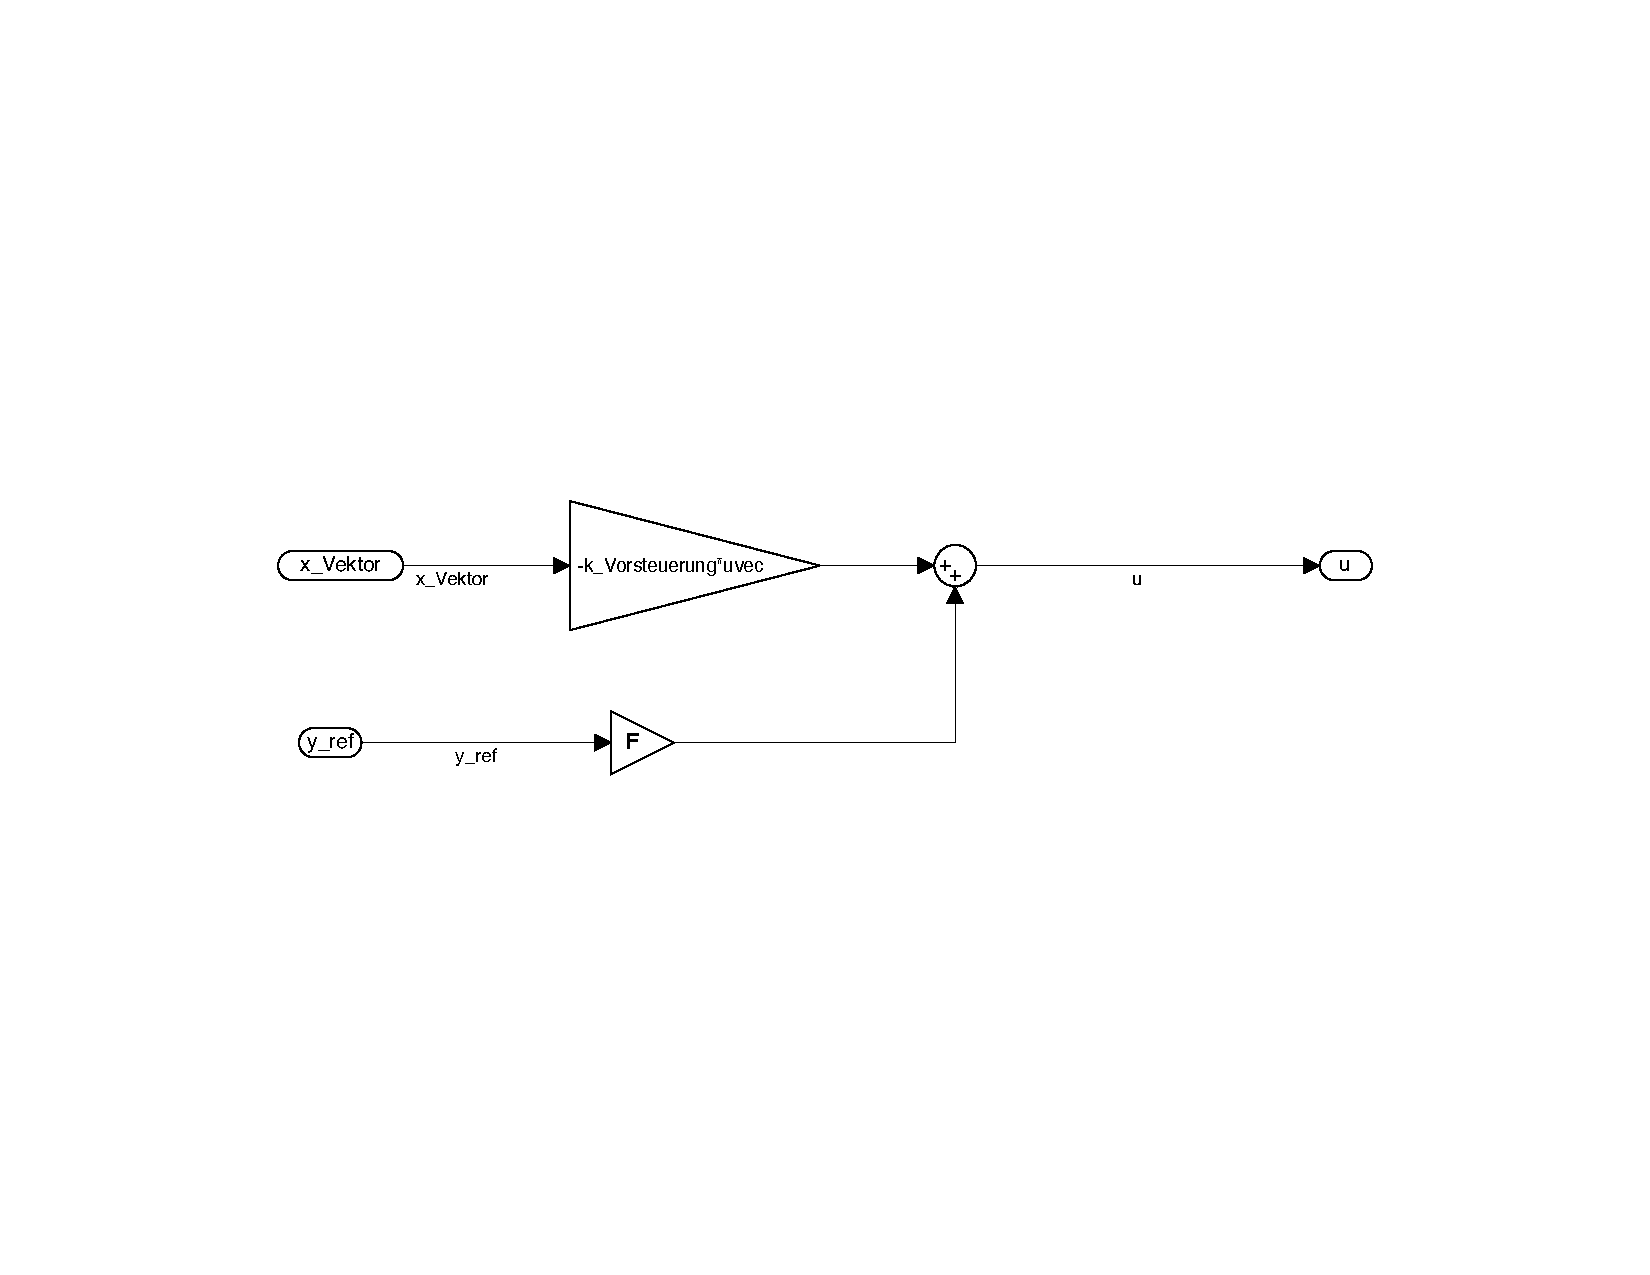
\includegraphics[width=1.0\textwidth]{Bilder/Reglervalidierung/Vorsteuerung_Regler.pdf}}
    \caption[Regler mit Vorsteuerung Simulink (linear)]{Simulink Regler-Blockschaltbild für den Zustandsregler mit Vorsteuerung (lineares Zustandsraummmodell)}
    \label{fig:Bild17}
\end{figure}

\begin{figure}[H]
    \centering
    \fbox{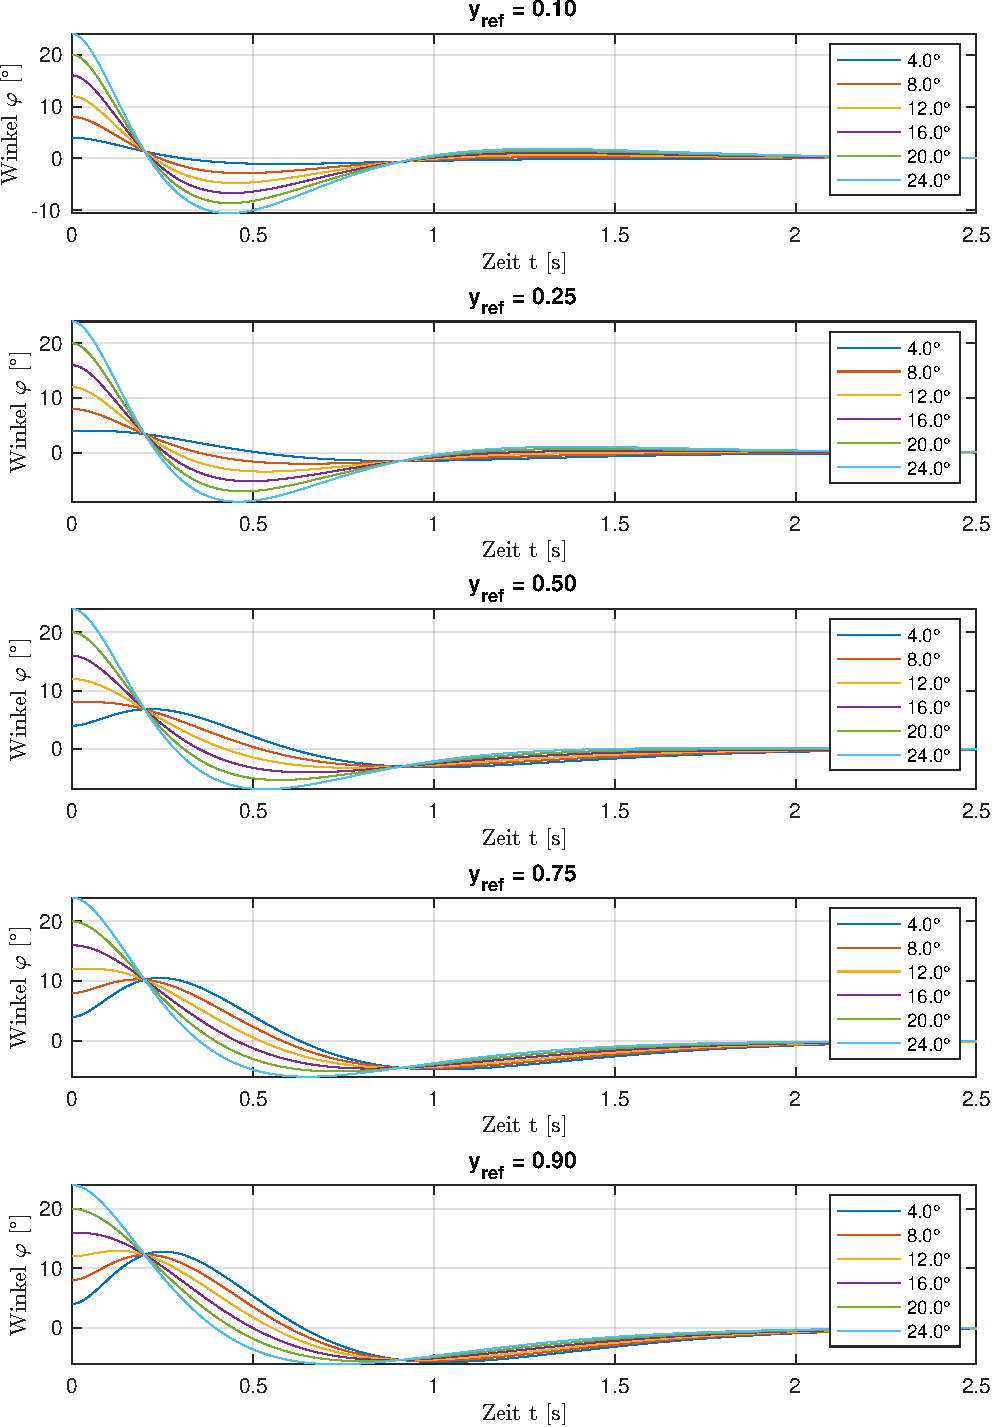
\includegraphics[width=0.8\textwidth]{Bilder/Reglervalidierung/linear_vorsteuerung_phi.pdf}}
    \caption[$\varphi$ für Regler mit Vorsteuerung (linear)]{$\varphi$ für verschiedene Referenzpositionen $y_{ref}$ und Anfangsauslenkungen am Zustandsregler mit Vorsteuerung für das lineare Zustandsraummodell}
    \label{fig:Bild18}
\end{figure}

\begin{figure}[H]
    \centering
    \fbox{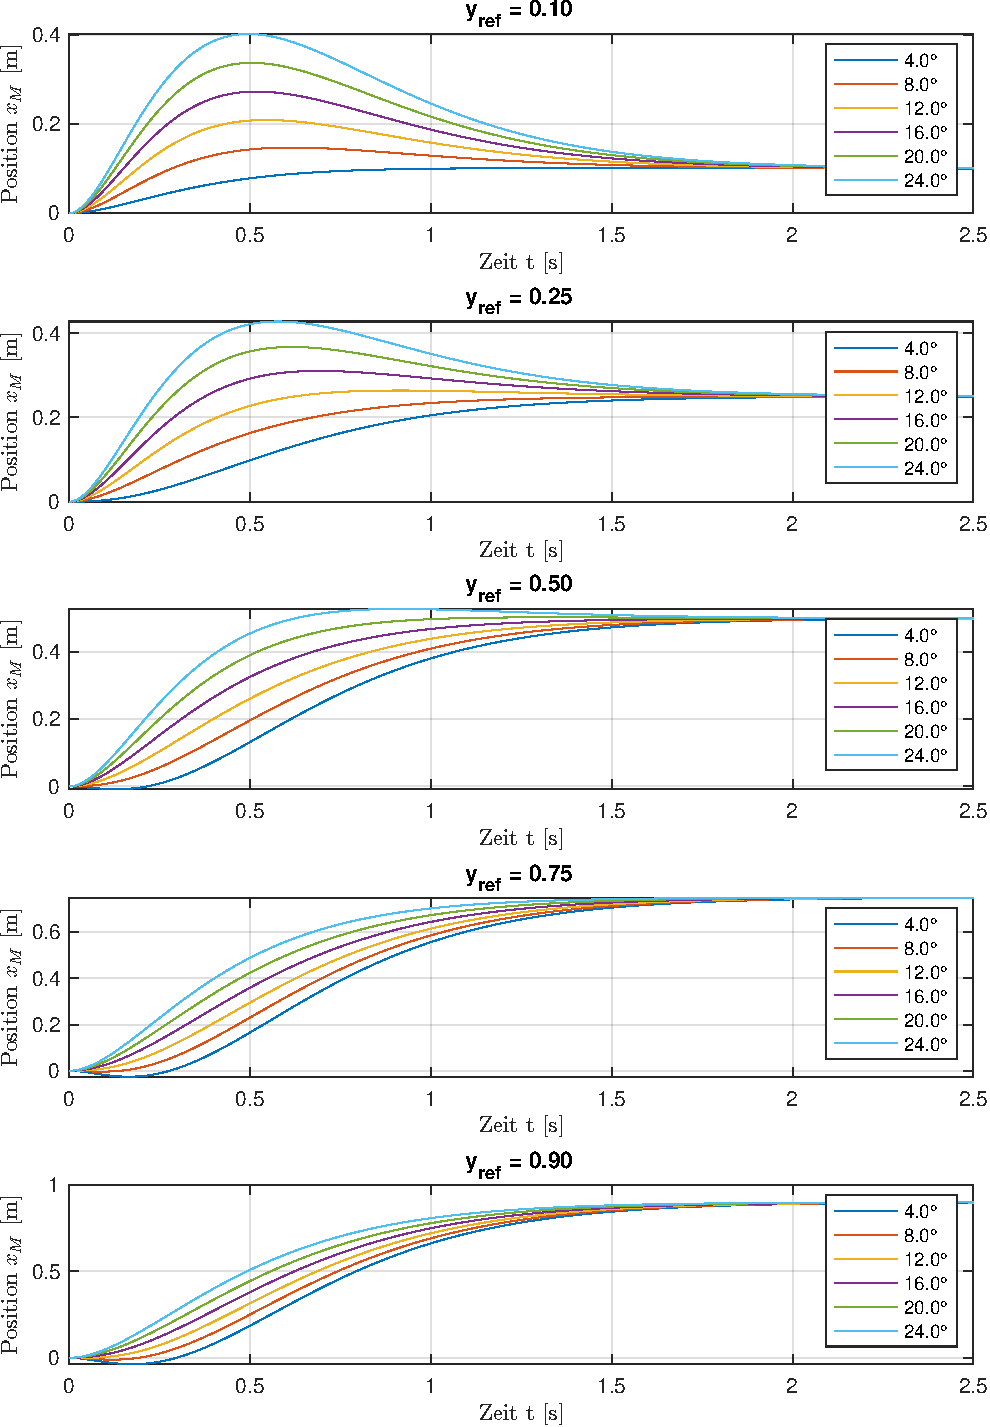
\includegraphics[width=0.8\textwidth]{Bilder/Reglervalidierung/linear_vorsteuerung_xM.pdf}}
    \caption[$x_{\mathrm{M}}$ für Regler mit Vorsteuerung (linear)]{$x_{\mathrm{M}}$ für verschiedene Referenzpositionen $y_{ref}$ und Anfangsauslenkungen am Zustandsregler mit Vorsteuerung für das lineare Zustandsraummodell}
    \label{fig:Bild19}
\end{figure}

\begin{figure}[H]
    \centering
    \fbox{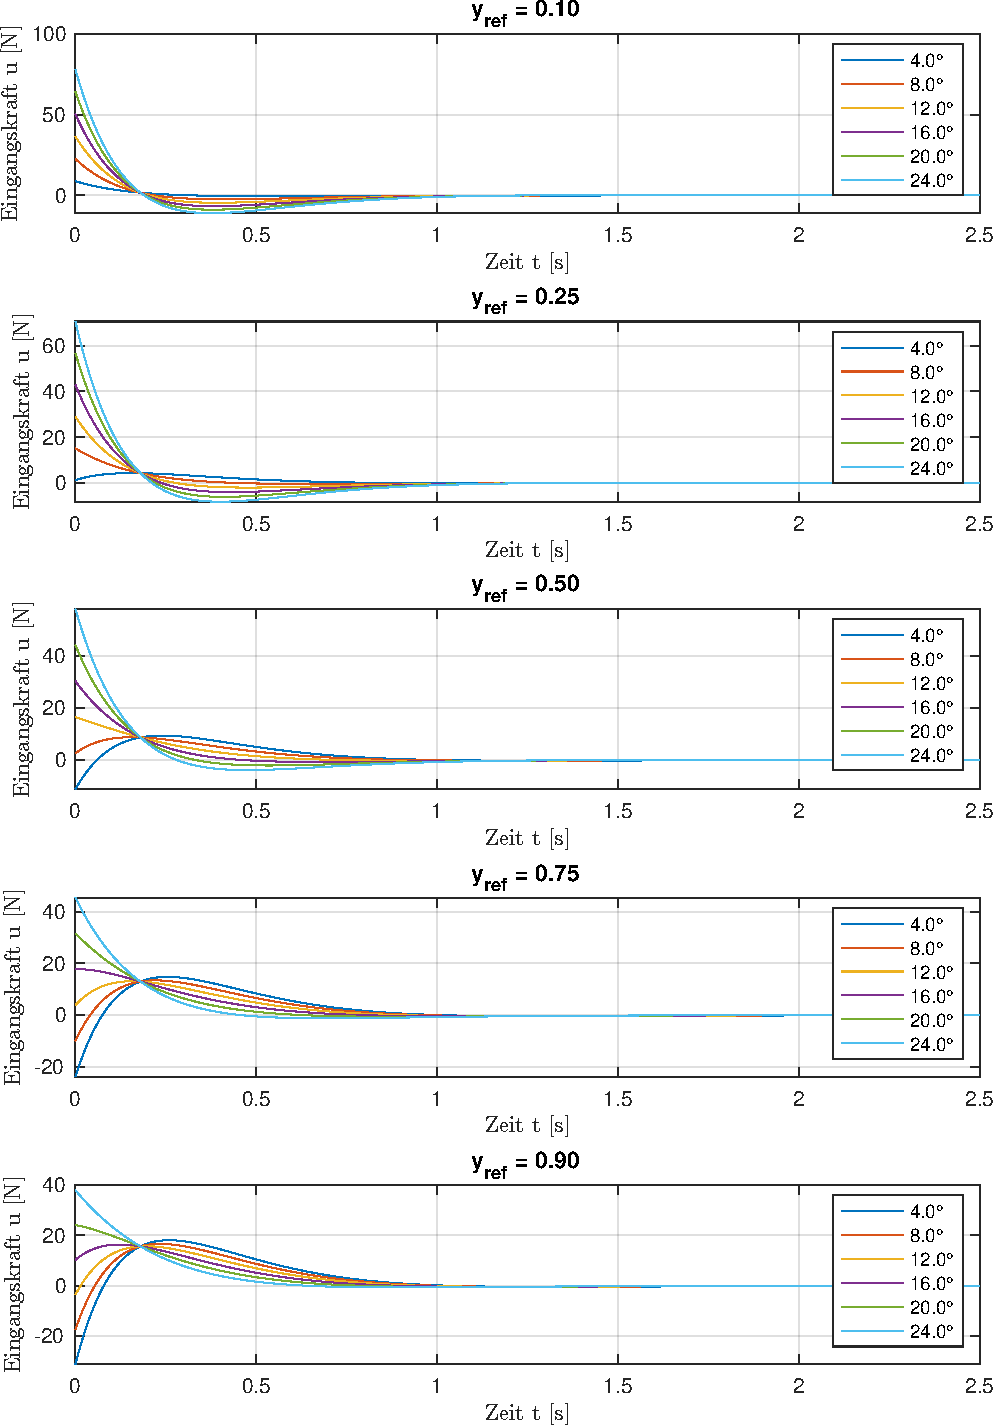
\includegraphics[width=0.8\textwidth]{Bilder/Reglervalidierung/linear_vorsteuerung_u.pdf}}
    \caption[u für Regler mit Vorsteuerung (linear)]{u für verschiedene Referenzpositionen $y_{ref}$ und Anfangsauslenkungen am Zustandsregler mit Vorsteuerung für das lineare Zustandsraummodell}
    \label{fig:Bild20}
\end{figure}

\newpage
Die für die oben gezeigten Diagramme gewählten Reglerpolstellen sind in \autoref{eq:Gleichung56} gezeigt. \\
\newline
\autoref{fig:Bild18} bestätigt analog zum Regler mit einfacher Zustandsrückführung (Ackermann-Formel), dass der Regler mit Vorsteuerung, wie definiert, eine Anfangsauslenkung zu $0^\circ$ (obere Ruhelage) ausregeln kann. Der Winkel ist nach \ca 2,5 s wieder in der Ruhelage angelangt. \\
\newline
Das Verhalten des Wagens ist gezeigt in \autoref{fig:Bild19}. Zu erkennen ist, dass je nach vorgegebenem Referenzwert die jeweilige Referenzposition am Ende des Regelvorgangs erreicht wird. Weiterhin bestätigt die Abbildung, dass selbst für einen Auslenkungswinkel von $24^\circ$ und eine Referenzposition von 0,9 m die maximale Wagenposition nicht überschritten wird. \\
\newline
Das dritte Diagramm (\autoref{fig:Bild20}) zeigt die benötigte Kraft des Motors am Schlitten, um den Wagen in entsprechender Zeit an die zuvor gezeigte Position zu bewegen. Zu erkennen ist, dass für größere Referenzpositionen bei großen Winkeln eine kleinere Eingangskraft benötigt wird. Dafür steigt jedoch bei kleinen Anfangsauslenkungen und großen Referenzwerten die benötigte Eingangskraft. In diesem Fall jedoch mit einem negativen Vorzeichen. Das beschriebene Verhalten entspricht den Erwartungen. Zuletzt ist festzuhalten, dass bereits nach rund 1,25 s der Motor keine Kraft mehr liefern muss.\\
\newline
Zusammenfassend kann bestätigt werden, dass sich der Regler erwartungsgemäß verhält und die Grenzen der Anlage bezüglich maximaler Position und Kraft nicht überschritten werden.

\subsubsection{Zustandsregler mit I-Regelung} \label{sec:val_i_regler}

Der dritte untersuchte Regler ist der Zustandsregler mit I-Regelung. Die Simulink-Struktur des Reglers ist in \autoref{fig:Bild21} gezeigt. Wie schon in \autoref{sec:val-vor} können Referenzpositionen vorgegeben werden. Im Unterschied zur Vorsteuerung soll jedoch durch das Aufintegrieren des Regelfehlers die Möglichkeit bestehen die Polstellen weiter nach Rechts zu schieben und somit den Regler zu beschleunigen. Dies gilt zu zeigen. \\
In Diagrammform werden erneut der Winkel des Pendels $\varphi$, die Wagenposition $x_{\mathrm{M}}$ und die benötigte Eingangskraft $u$ \bzw $F_{\mathrm{a}}$ dargestellt. Zusätzlich wird die Validierung für verschiedene Referenzpositionen $y_{ref}$ vorgenommen. \\
Ziel ist auch hier das Bestätigen des Einhaltens der Grenzen der Anlage für die gewählten Polstellen bei untersuchten Anfangsauslenkungen und Referenzpositionen. 

\begin{figure}[H]
    \centering
    \fbox{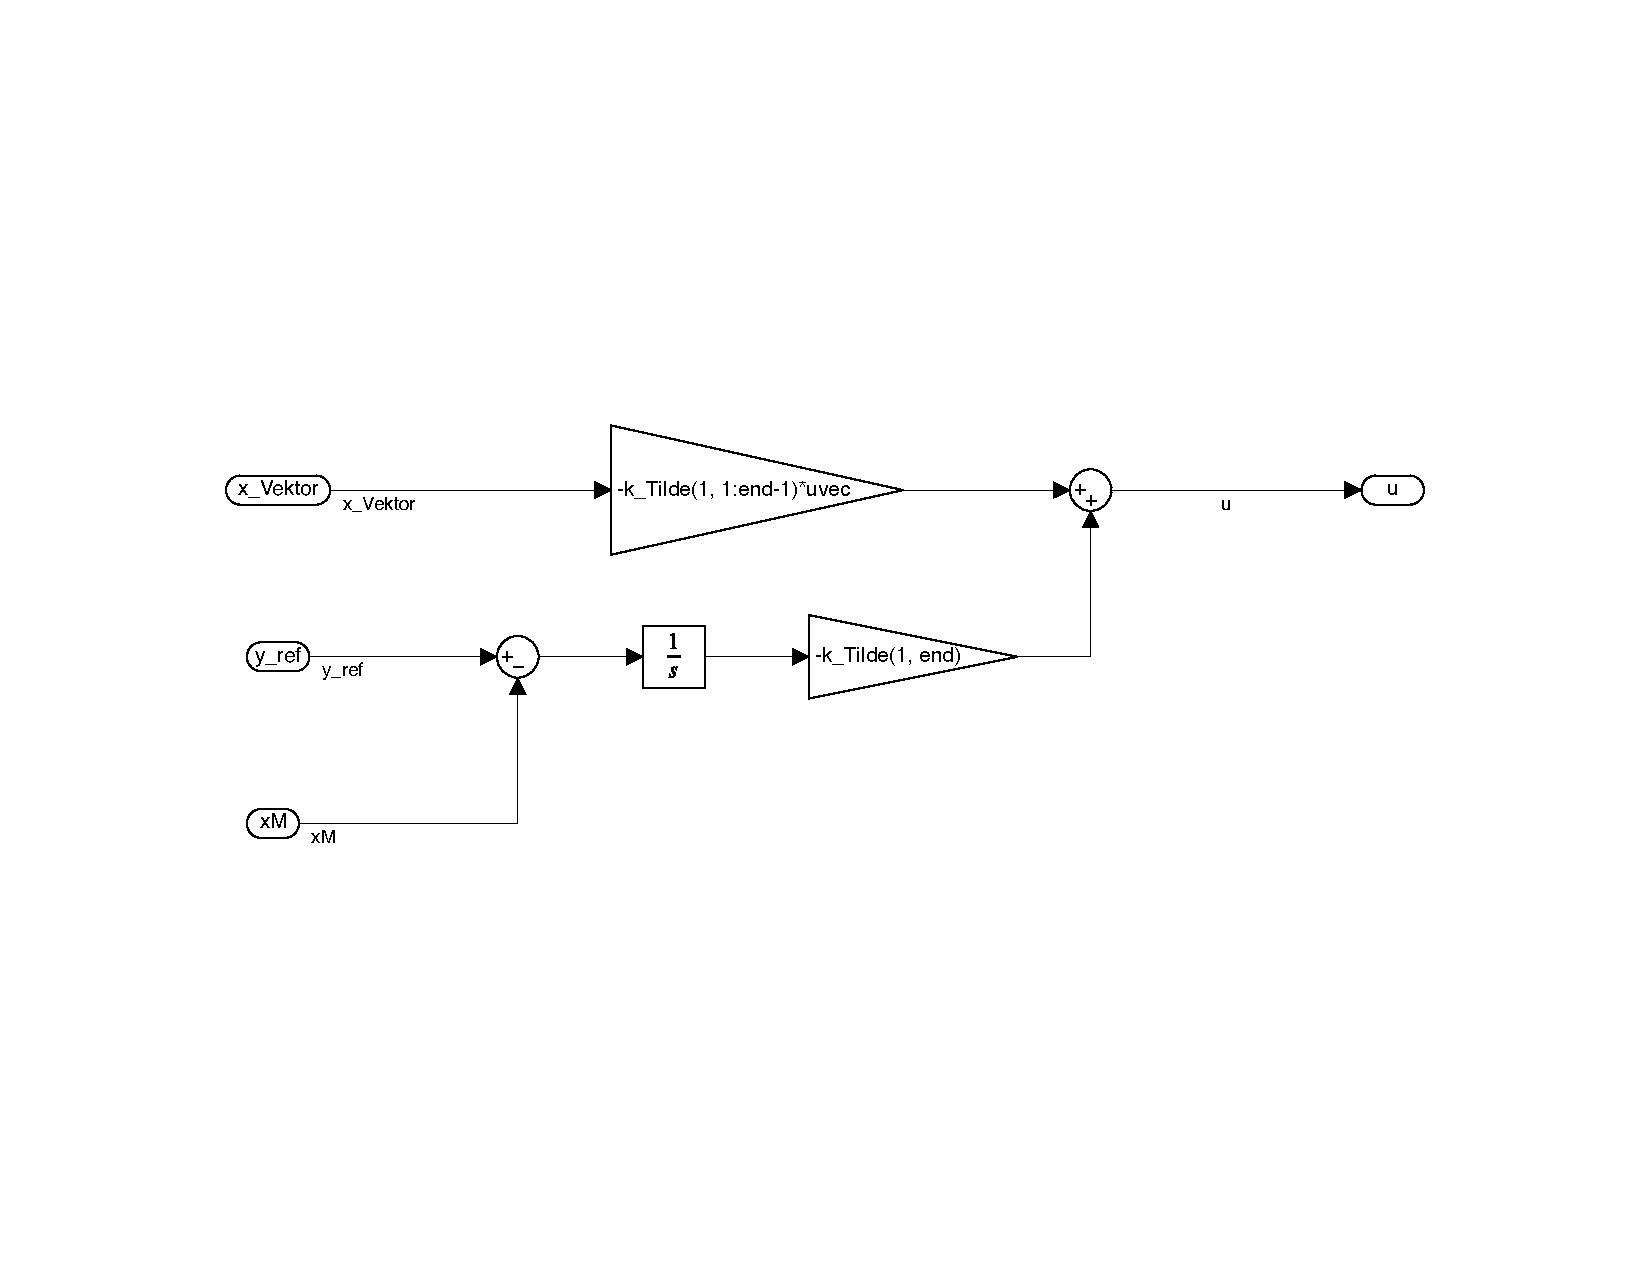
\includegraphics[width=1.0\textwidth]{Bilder/Reglervalidierung/I_Regler.pdf}}
    \caption[Regler mit I-Regelung Simulink (linear)]{Simulink Regler-Blockschaltbild für den Zustandsregler mit I-Regelung (lineares Zustandsraummodell)}
    \label{fig:Bild21}
\end{figure}

Die für die nachfolgend gezeigten Diagramme gewählten Reglerpolstellen sind in \autoref{eq:Gleichung67} gezeigt. \\
\newline
\autoref{fig:Bild22} bestätigt analog zu den vorangegangenen Reglern, dass der I-Regler wie definiert eine Anfangsauslenkung zu $0^\circ$ (obere Ruhelage) ausregeln kann. Der Winkel ist nach \ca 2,5 s wieder in der Ruhelage angelangt. \\
\newline
Das Verhalten des Wagens ist gezeigt in \autoref{fig:Bild23}. Zu erkennen ist, dass je nach vorgegebenem Referenzwert die jeweilige Referenzposition am Ende des Regelvorgangs erreicht wird. Der Vorgang braucht jedoch merklich länger mit rund 3,5 s. \\
\newline
Das dritte Diagramm (\autoref{fig:Bild24}) zeigt die benötigte Kraft des Motors, um den Wagen an die zuvor gezeigte Position zu bewegen. Zu erkennen ist, dass für größere Referenzpositionen bei großen Winkeln eine kleinere Eingangskraft benötigt wird. Dafür steigt jedoch bei kleinen Anfangsauslenkungen und großen Referenzwerten die benötigte Eingangskraft. In diesem Fall jedoch mit einem negativen Vorzeichen. Zuletzt ist festzuhalten, dass bereits nach rund 1,25 s der Motor keine Kraft mehr liefern muss.\\
\newline
Zusammenfassend kann bestätigt werden, dass sich der Regler bei festgelegten Polstellen immer noch erwartungsgemäß verhält und die Grenzen der Anlage bezüglich maximaler Position und Kraft nicht überschritten werden.

\begin{figure}[H]
    \centering
    \fbox{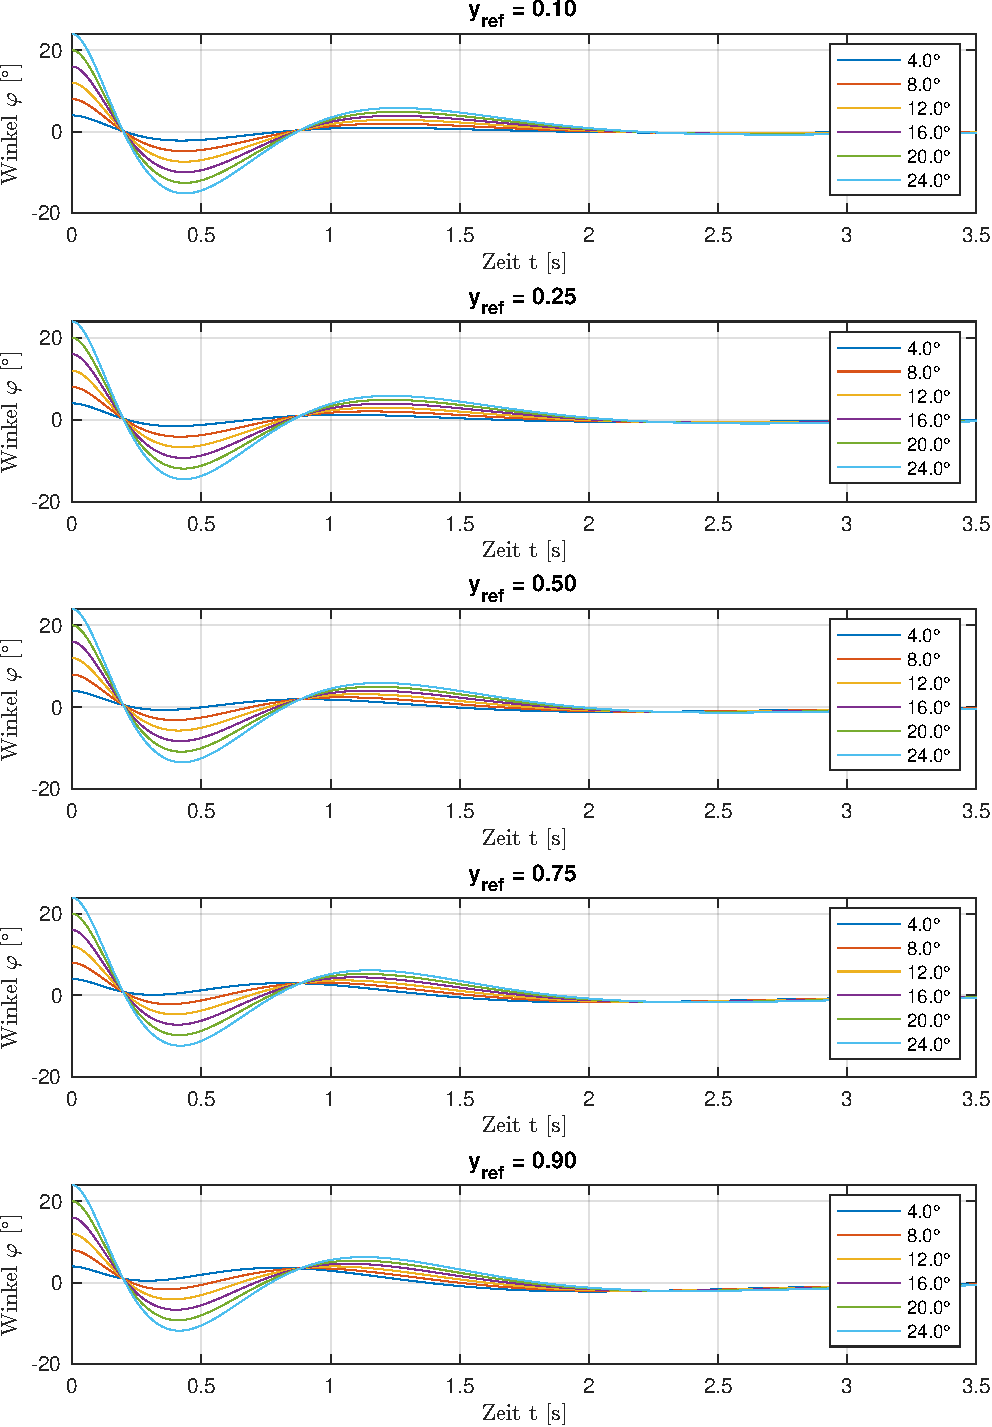
\includegraphics[width=0.8\textwidth]{Bilder/Reglervalidierung/linear_i_regler_phi.pdf}}
    \caption[$\varphi$ für Regler mit I-Regelung (linear)]{$\varphi$ für verschiedene Referenzpositionen $y_{ref}$ und Anfangsauslenkungen am Zustandsregler mit I-Regelung für das lineare Zustandsraummodell}
    \label{fig:Bild22}
\end{figure}

\begin{figure}[H]
    \centering
    \fbox{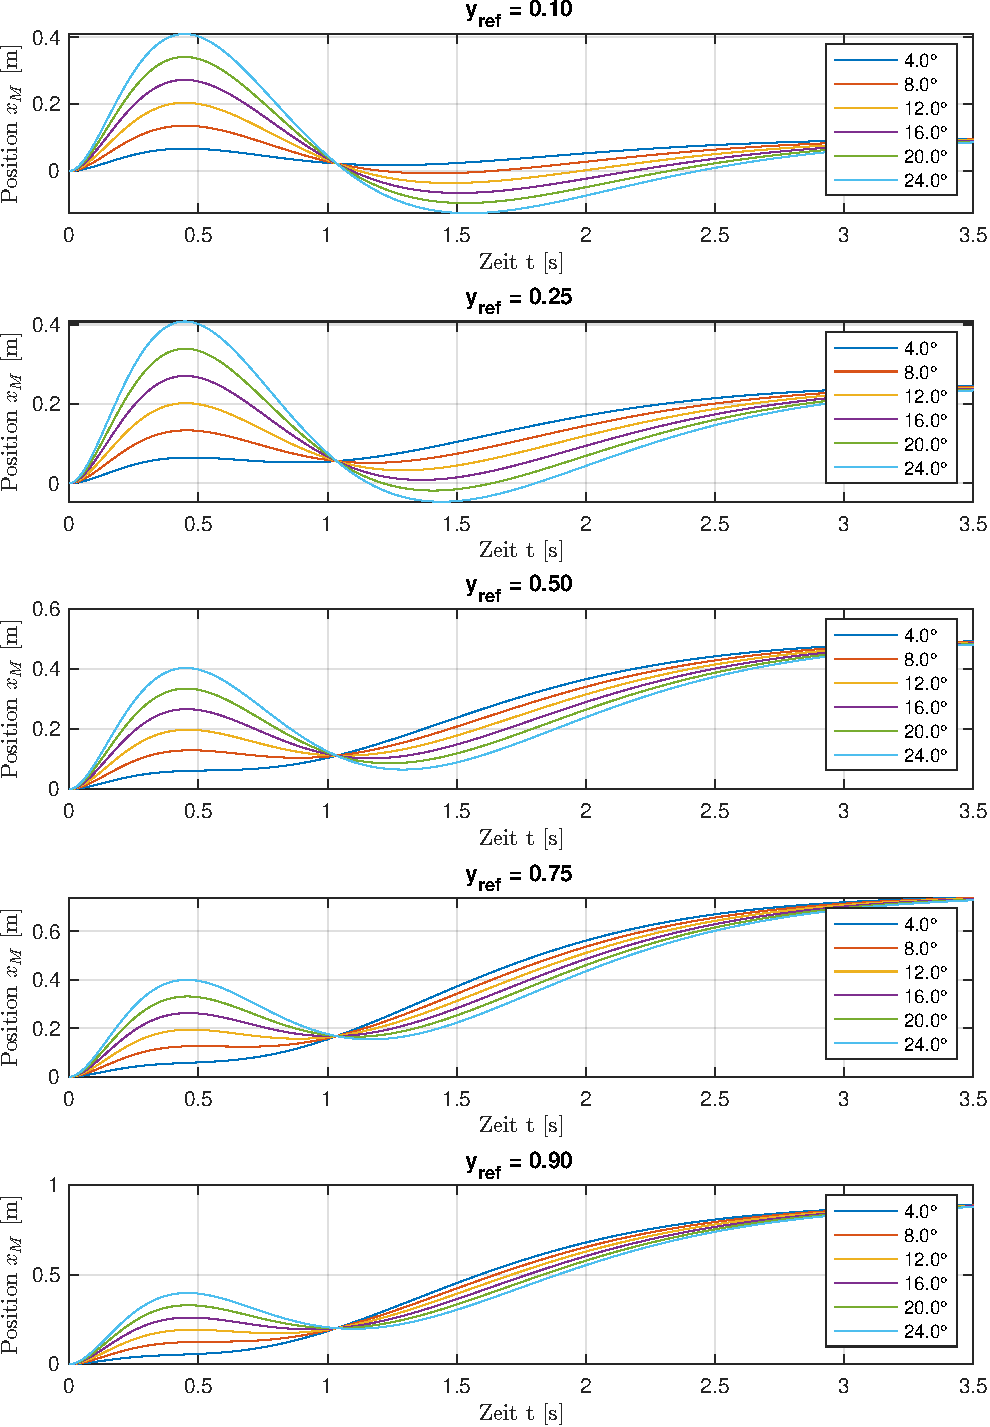
\includegraphics[width=0.8\textwidth]{Bilder/Reglervalidierung/linear_i_regler_xM.pdf}}
    \caption[$x_{\mathrm{M}}$ für Regler mit I-Regelung (linear)]{$x_{\mathrm{M}}$ für verschiedene Referenzpositionen $y_{ref}$ und Anfangsauslenkungen am Zustandsregler mit I-Regelung für das lineare Zustandsraummodell}
    \label{fig:Bild23}
\end{figure}

\begin{figure}[H]
    \centering
    \fbox{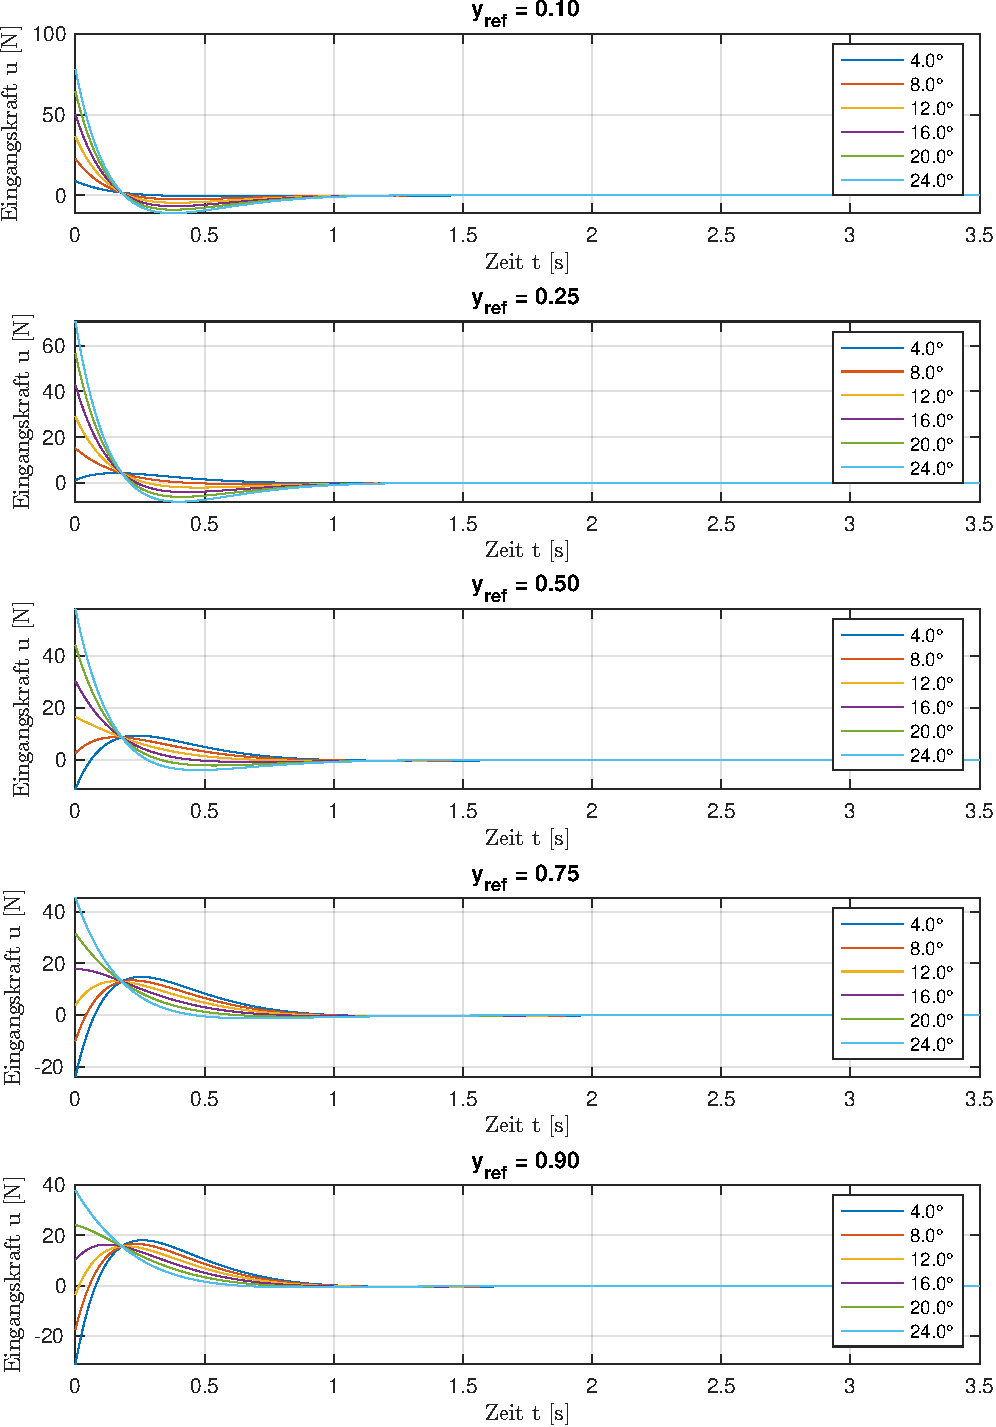
\includegraphics[width=0.8\textwidth]{Bilder/Reglervalidierung/linear_i_regler_u.pdf}}
    \caption[u für Regler mit I-Regelung (linear)]{u für verschiedene Referenzpositionen $y_{ref}$ und Anfangsauslenkungen am Zustandsregler mit I-Regelung für das lineare Zustandsraummodell}
    \label{fig:Bild24}
\end{figure}

\subsubsection{Vergleich des Regelverhaltens}

Im folgenden werden die drei implementierten Regelstrategien verglichen. Dabei soll herausgearbeitet werden, welche Vorteile für einen bestimmten Regler sprechen und welcher am geeignetsten für die Regelaufgabe ist. \\
Um eine gewisse Vergleichbarkeit sicherzustellen, wurden alle drei Simulink-Modelle der Regler inklusive Regelstrecke mit der gleichen Anfangsauslenkung simuliert. Weiterhin wurde auch die selbe Referenzposition beim Zustandsregler mit Vorsteuerung und beim Regler mit I-Regelung genutzt. \\
In Diagrammform werden nachfolgend der Winkel des Pendels $\varphi$, die Wagenposition $x_{\mathrm{M}}$ und die benötigte Eingangskraft $u$ \bzw $F_{\mathrm{a}}$ für die drei Zustandsregler dargestellt. \\
Es ist wichtig die gewählten Polstellen für den jeweiligen Regler zu berücksichtigen und diese mit in den Vergleich einzubeziehen. Nachfolgen sind die Polstellen aufgeführt:
\begin{align*}
    \underline{s}_{\mathrm{P}_{Acker.}} &= 
    \begin{bmatrix}
        -4.0 & -4.0 & -4.0 & -4.0 
    \end{bmatrix} \\
    \underline{s}_{\mathrm{P}_{Vorst.}} &= 
    \begin{bmatrix}
        -4.5 & -4.5 & -4.5 & -4.5 
    \end{bmatrix} \\
    \underline{s}_{\mathrm{P}_{I-Reg.}} &= 
    \begin{bmatrix}
        -3.2 & -3.2 & -3.2 & -3.2 
    \end{bmatrix}
\end{align*}
\newline
Die Wahl der Polstellen beruht auf der Optimierung der Regelgeschwindigkeit bei maximalem Ausreizen der Systemgrenzen.

\begin{figure}[H]
    \centering
    \fbox{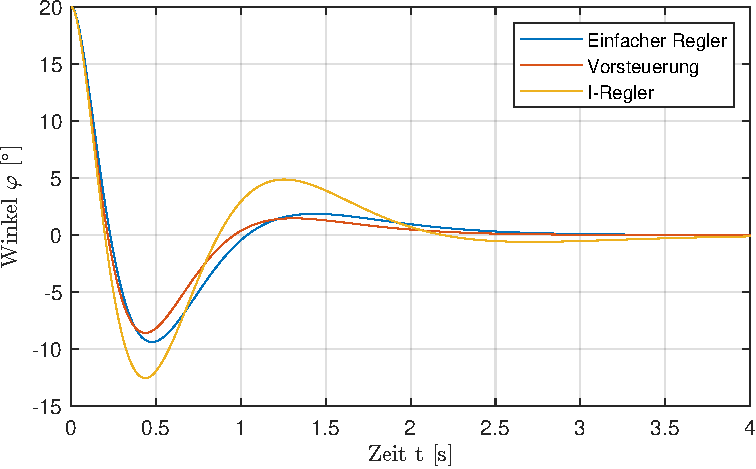
\includegraphics[width=0.65\textwidth]{Bilder/Reglervalidierung/linear_vergleich_phi.pdf}}
    \caption[Reglervergleich für $\varphi$ (linear)]{$\varphi$ für Regler mit einfacher Zustandsrückführung, Regler mit Vorsteuerung und Regler mit I-Regelung bei einer Anfangsauslenkungen von $20^\circ$ und einer Referenzposition $y_{ref} = 0,1 m$ am linearen Zustandsraummodell}
    \label{fig:Bild25}
\end{figure}

\begin{figure}[H]
    \centering
    \fbox{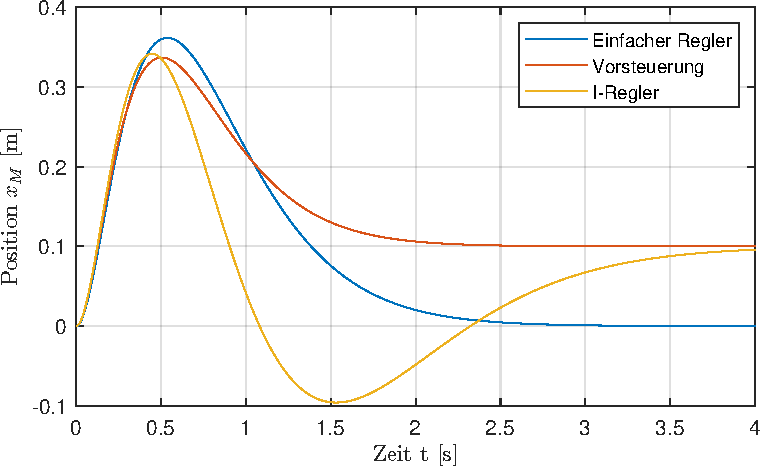
\includegraphics[width=0.65\textwidth]{Bilder/Reglervalidierung/linear_vergleich_xM.pdf}}
    \caption[Reglervergleich für $x_{\mathrm{M}}$ (linear)]{$x_{\mathrm{M}}$ für Regler mit einfacher Zustandsrückführung, Regler mit Vorsteuerung und Regler mit I-Regelung bei einer Anfangsauslenkungen von $20^\circ$ und einer Referenzposition $y_{ref} = 0,1 m$ am linearen Zustandsraummodell}
    \label{fig:Bild26}
\end{figure}

\begin{figure}[H]
    \centering
    \fbox{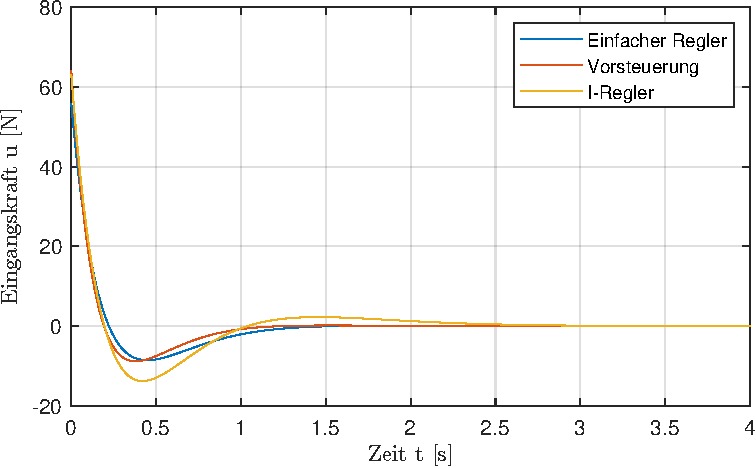
\includegraphics[width=0.65\textwidth]{Bilder/Reglervalidierung/linear_vergleich_u.pdf}}
    \caption[Reglervergleich für $u$ (linear)]{$u$ für Regler mit einfacher Zustandsrückführung, Regler mit Vorsteuerung und Regler mit I-Regelung bei einer Anfangsauslenkungen von $20^\circ$ und einer Referenzposition $y_{ref} = 0,1 m$ am linearen Zustandsraummodell}
    \label{fig:Bild27}
\end{figure}

\autoref{fig:Bild25} zeigt, dass der Winkel des Pendels bei der Regelung mit Vorsteuerung für die oben gewählten Polstellen am schnellsten wieder in der Ruhelage ausgeregelt ist. Dieses Verhalten lässt sich dadurch begründen, dass die Polstellen bei der Vorsteuerung etwas weiter nach links gelegt wurden im Vergleich zum Regler mit einfacher Zustandsrückführung, wodurch der Regler schneller wird. Grundsätzlich würden die Kurvenverläufe der beiden genannten Regler annähernd identisch sein, wenn die Polstellen die gleichen sind und bei der Vorsteuerung die Referenzposition zu Null gewählt wird. Verschiebt man bei positiver Anfangsauslenkung jedoch die Referenzposition nach rechts, so würde der Regler mit Vorsteuerung deutlich schneller wieder in die Ruhelage regeln, da er nicht dafür sorgen muss, dass der Wagen wieder auf der Nullposition stehen bleibt. Der Zustandsregler mit I-Regelung scheint im Gegensatz generell etwas langsamer zu sein, selbst wenn die Polstellen für alle Regelstrategien gleich gewählt werden. \\
Weiterhin ist zu erkennen, das bei der I-Regelung ein stärkeres Schwingen auftritt, welches durch das Aufintegrieren des Regelfehlers zu erklären ist. \\
\newline
In \autoref{fig:Bild26} ist vor allem der wesentliche Unterschied zwischen dem Regler mit einfacher Zustandsrückführung und den Reglern mit Zustandsrückführung und Referenzwertvorgabe zu erkennen. Bei der Vorsteuerung und I-Regelung kann in den jeweiligen Graphen die gewählte Referenzposition am rechten Ende des Diagramms abgelesen werden. Der einfache Zustandsregler regelt die Wagenposition wieder auf Null zurück. \\
Auch hier kann das stärkere Schwingverhalten des I-Reglers identifiziert werden. \\
\newline
Der wesentliche Grund für die Wahl der Polstellen wird in \autoref{fig:Bild27} ersichtlich. Für eine einheitliche Auslenkung des Pendels ist die Eingangskraft $u$ annähernd gleich bei den drei Reglern. Für die in den vorangegangenen Unterabschnitten ermittelten maximalen Auslenkungen ist die Eingangskraft $u$ \bzw $F_{\mathrm{a}}$ im Maximum knapp unter 80 N groß. Somit wird das System bei den gewählten Polstellen maximal ausgereizt. \\
Wie auch schon bei der Betrachtung des Winkels $\varphi$ und der Wagenposition $x_{\mathrm{M}}$ kann ein stärkeres Schwingungsverhalten beim Zustandsregler mit I-Regelung erkannt werden.

\newpage

\subsection{Validierung des nichtlinearen Modells}
Im folgenden werden die drei Regler für das nichtlineare Zustandsraummodell validiert. Die Simulink Implementierung der nichtlinearen Regelstrecke ist in \autoref{fig:Bild2} dargestellt. \\
\newline
Wie im vorangegangenen Unterabschnitt werden Diagramme für den Winkel des Pendels $\varphi$, die Wagenposition $x_{\mathrm{M}}$ und die benötigte Eingangskraft $u$ \bzw $F_{\mathrm{a}}$ für die drei Zustandsregler gezeigt. Es wird jedoch auf Kommentare verzichtet, da die Anwendung der Regler auf das nichtlineare Zustandsraummodell zu analogen Ergebnissen führt, was bereits in \autoref{sec:systemvergleich} nachgewiesen wurde.

\subsubsection{Zustandsregler mit einfacher Rückführung}

\begin{figure}[H]
    \centering
    \fbox{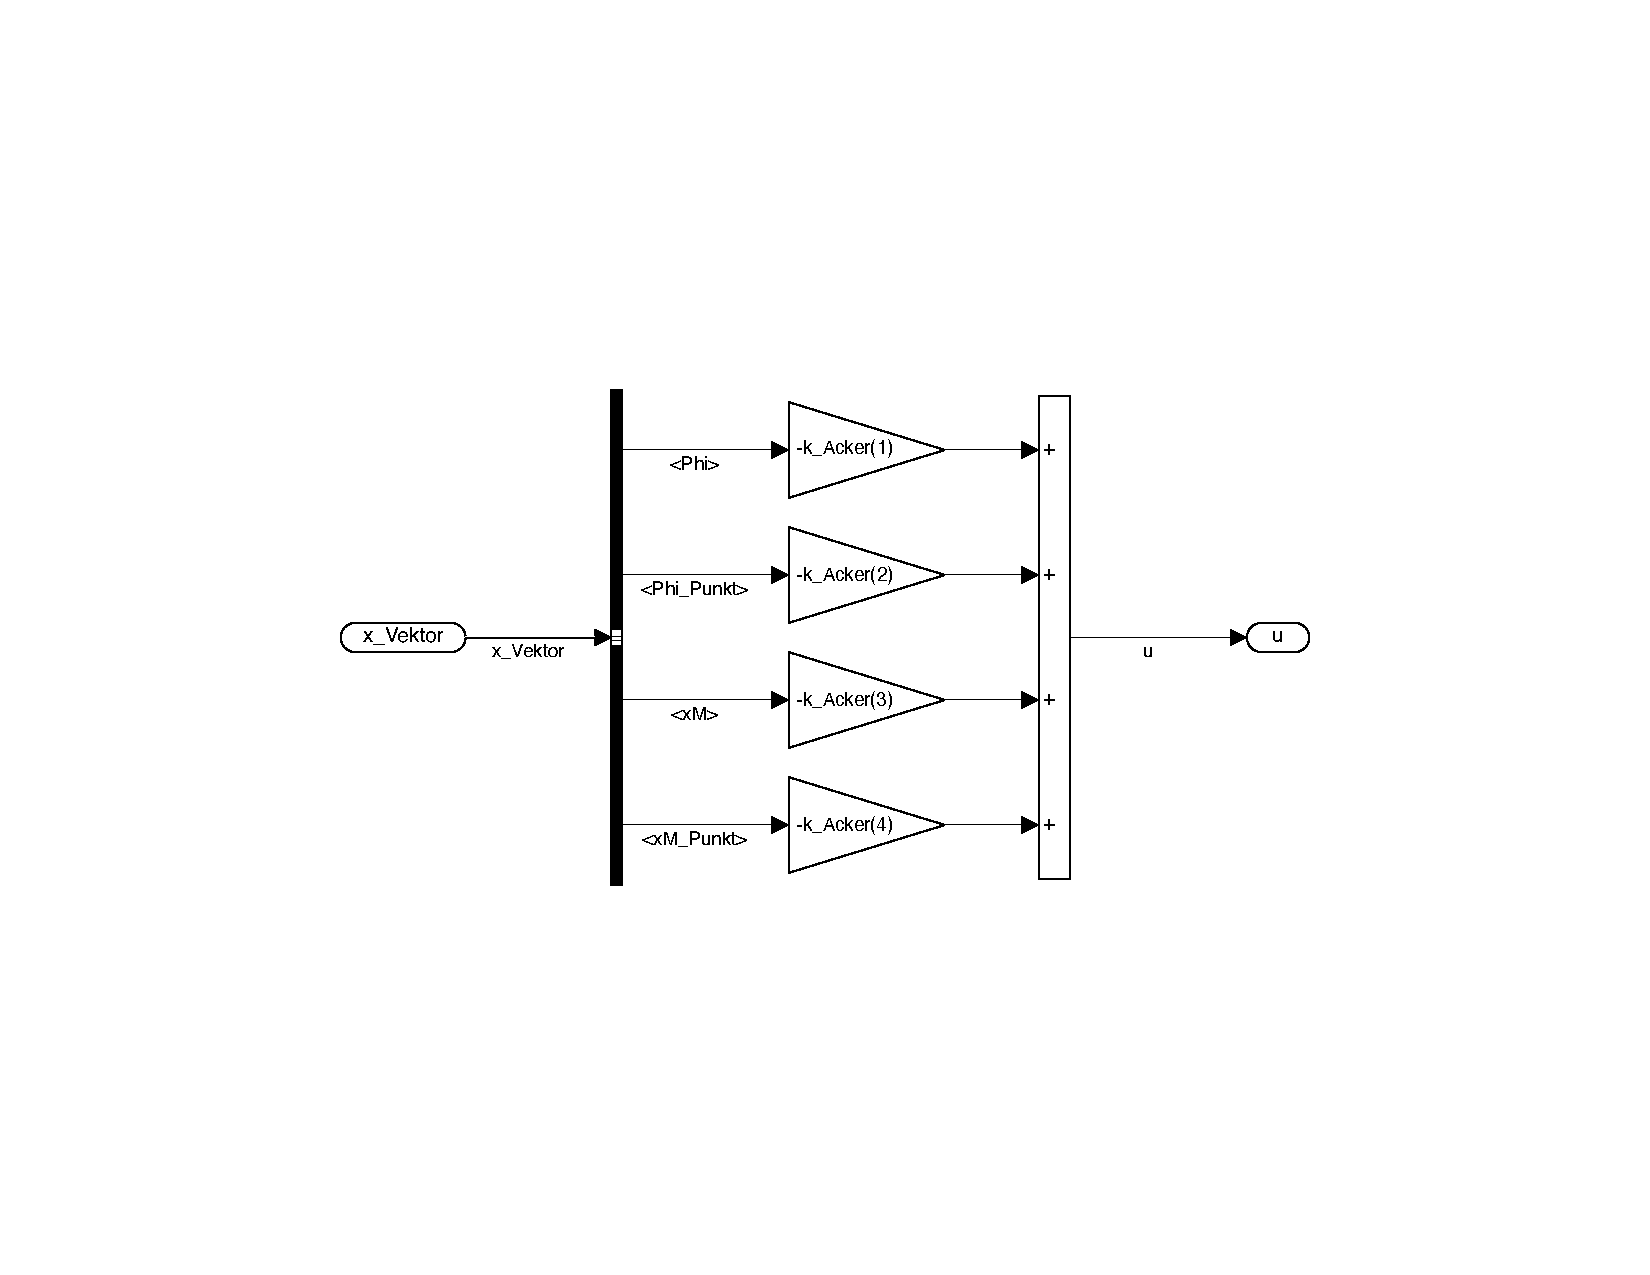
\includegraphics[width=1.0\textwidth]{Bilder/Reglervalidierung/Ackermann_Regler_nl.pdf}}
    \caption[Zustandsregler mit einfacher Rückführung - Simulink (nichtlinear)]{Simulink Regler-Blockschaltbild für den Zustandsregler mit einfacher Zustandsrückführung (nichtlineares Zustandsraummodell)}
    \label{fig:Bild28}
\end{figure}

\begin{figure}[H]
    \centering
    \fbox{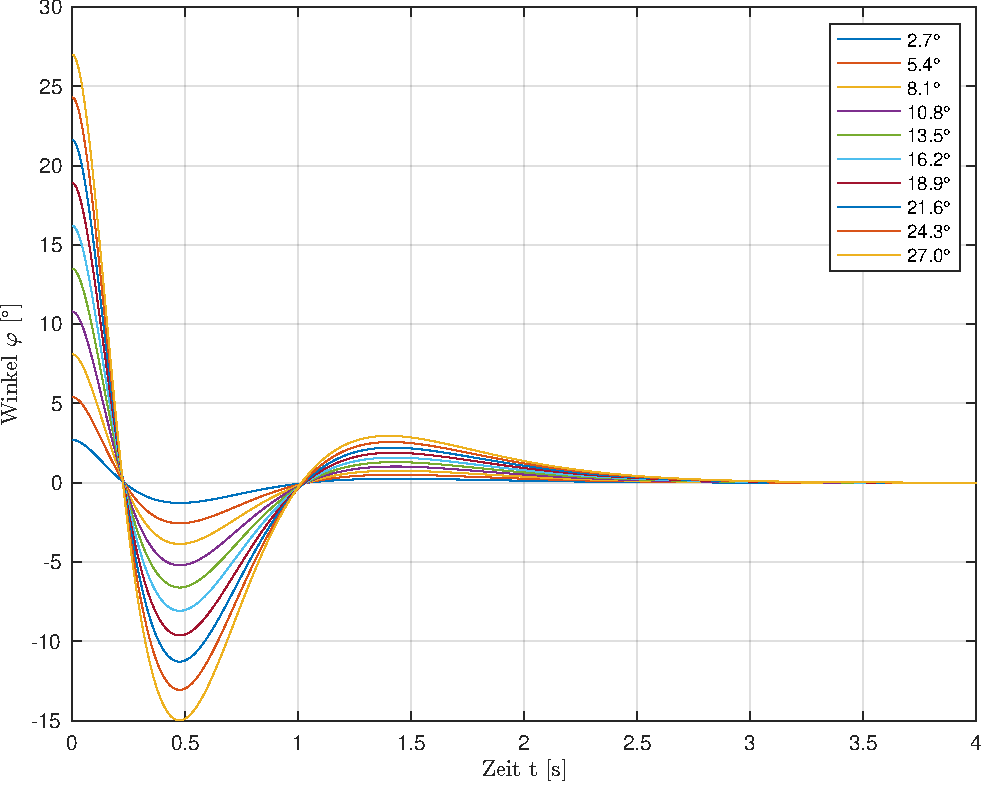
\includegraphics[width=0.6\textwidth]{Bilder/Reglervalidierung/nichtlinear_ackermann_phi.pdf}}
    \caption[$\varphi$ für Regler mit einfacher Rückführung (nichtlinear)]{$\varphi$ für verschiedene Anfangsauslenkungen am Zustandsregler mit einfacher Rückführung für das nichtlineare Zustandsraummodell}
    \label{fig:Bild29}
\end{figure}

\begin{figure}[H]
    \centering
    \fbox{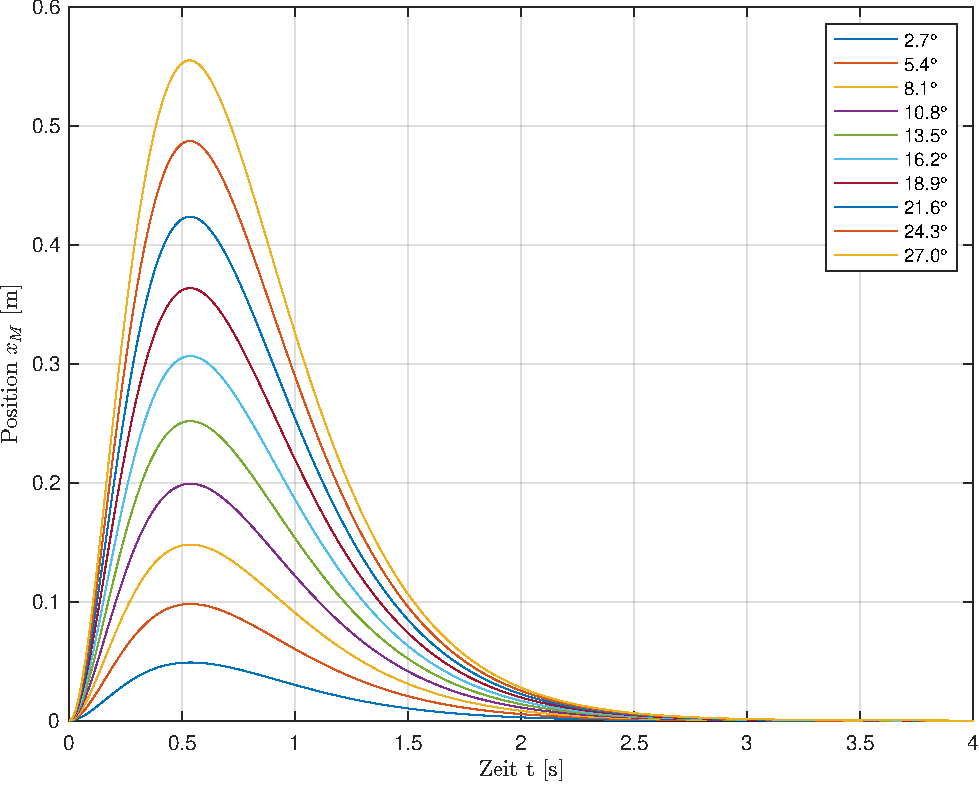
\includegraphics[width=0.6\textwidth]{Bilder/Reglervalidierung/nichtlinear_ackermann_xM.pdf}}
    \caption[$x_{\mathrm{M}}$ für Regler mit einfacher Rückführung (nichtlinear)]{$x_{\mathrm{M}}$ für verschiedene Anfangsauslenkungen am Zustandsregler mit einfacher Rückführung für das nichtlineare Zustandsraummodell}
    \label{fig:Bild30}
\end{figure}

\begin{figure}[H]
    \centering
    \fbox{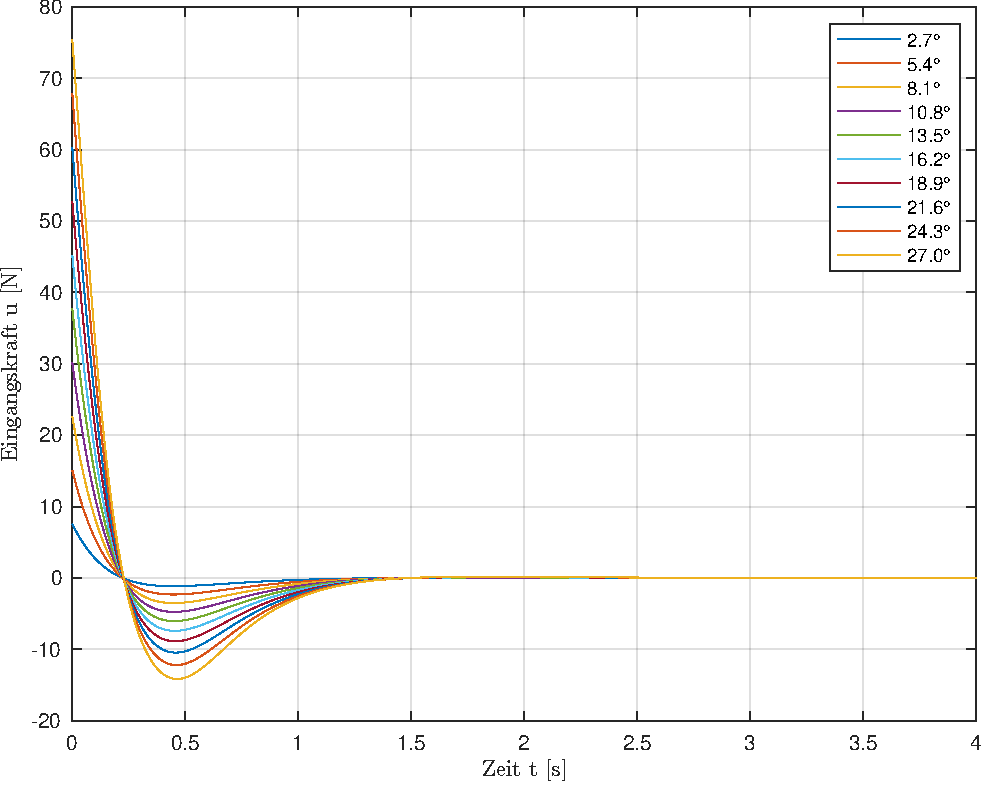
\includegraphics[width=0.6\textwidth]{Bilder/Reglervalidierung/nichtlinear_ackermann_u.pdf}}
    \caption[u für Regler mit einfacher Rückführung (nichtlinear)]{u für verschiedene Anfangsauslenkungen am Zustandsregler mit einfacher Rückführung für das nichtlineare Zustandsraummodell}
    \label{fig:Bild31}
\end{figure}

\subsubsection{Zustandsregler mit Vorsteuerung}

\begin{figure}[H]
    \centering
    \fbox{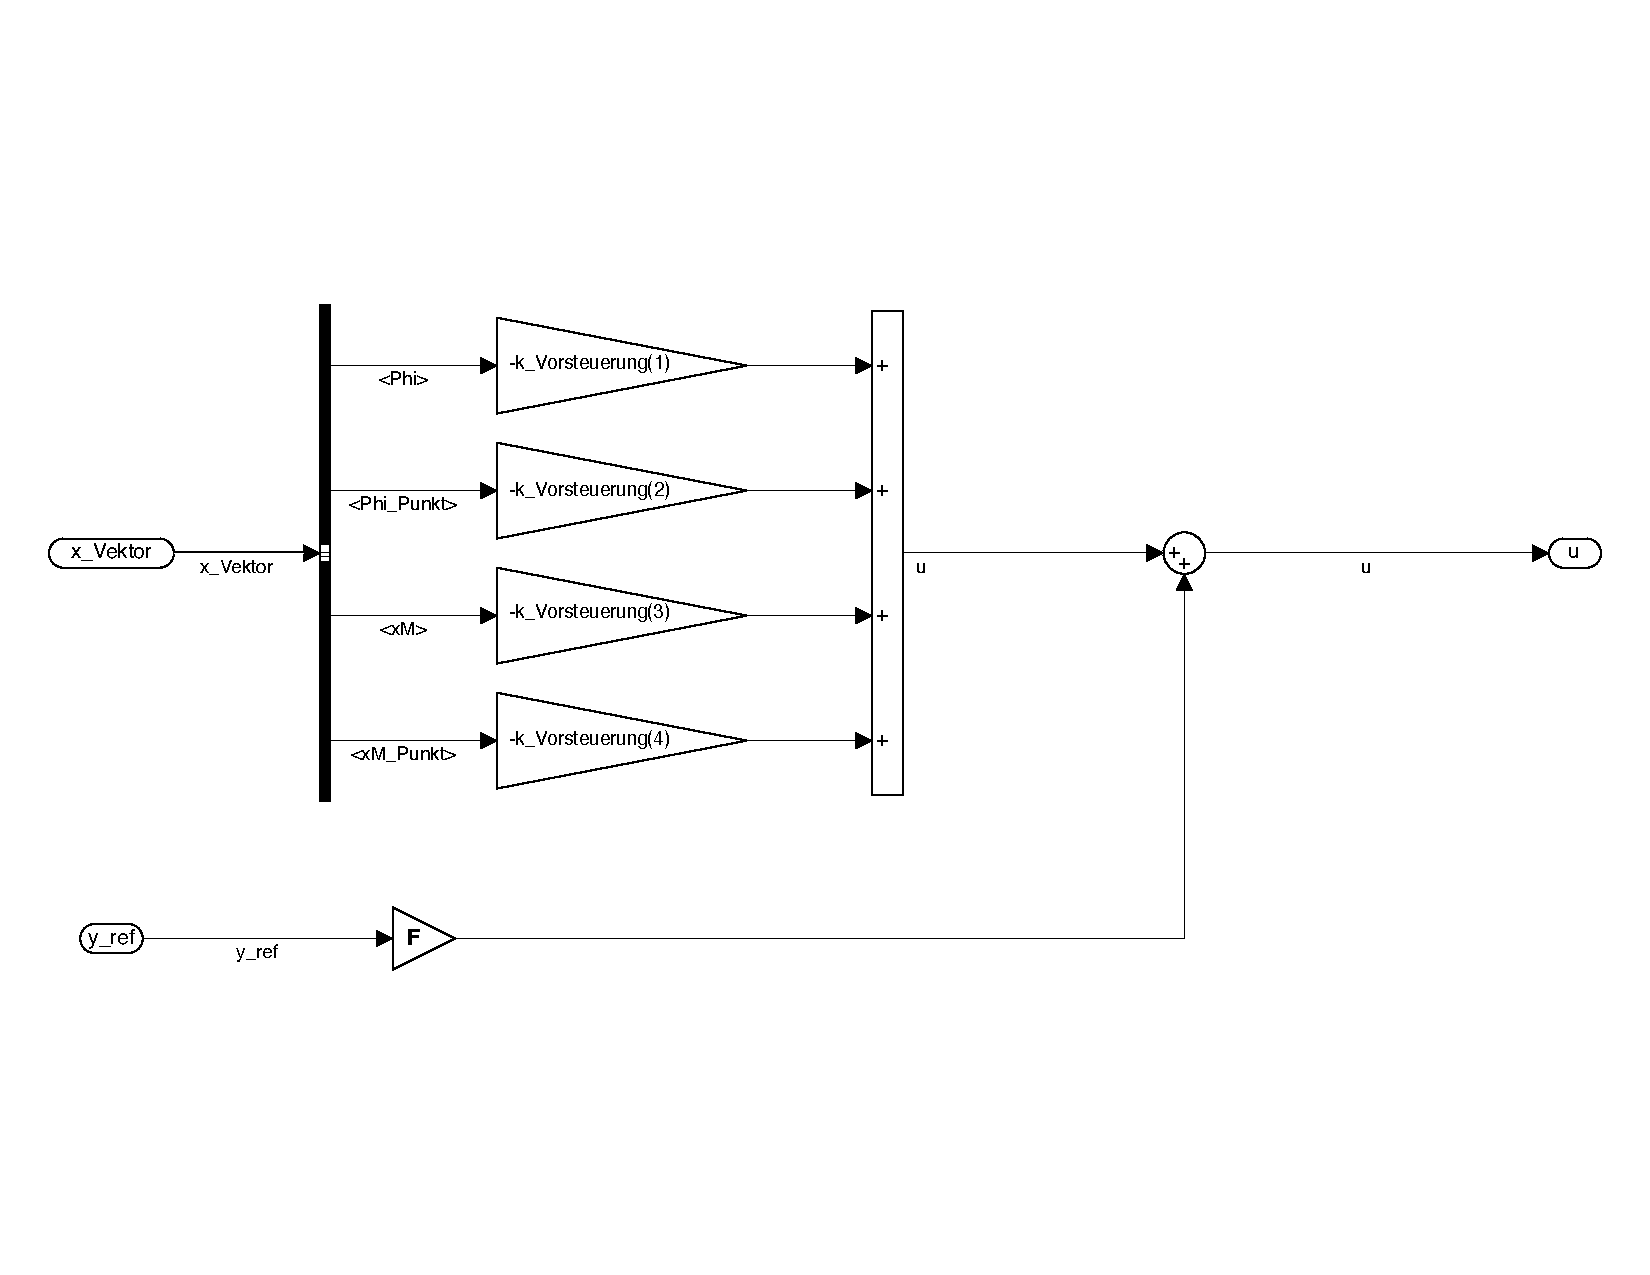
\includegraphics[width=1.0\textwidth]{Bilder/Reglervalidierung/Vorsteuerung_Regler_nl.pdf}}
    \caption[Regler mit Vorsteuerung Simulink (nichtlinear)]{Simulink Regler-Blockschaltbild für den Zustandsregler mit Vorsteuerung (nichtlineares Zustandsraummodell)}
    \label{fig:Bild32}
\end{figure}

\begin{figure}[H]
    \centering
    \fbox{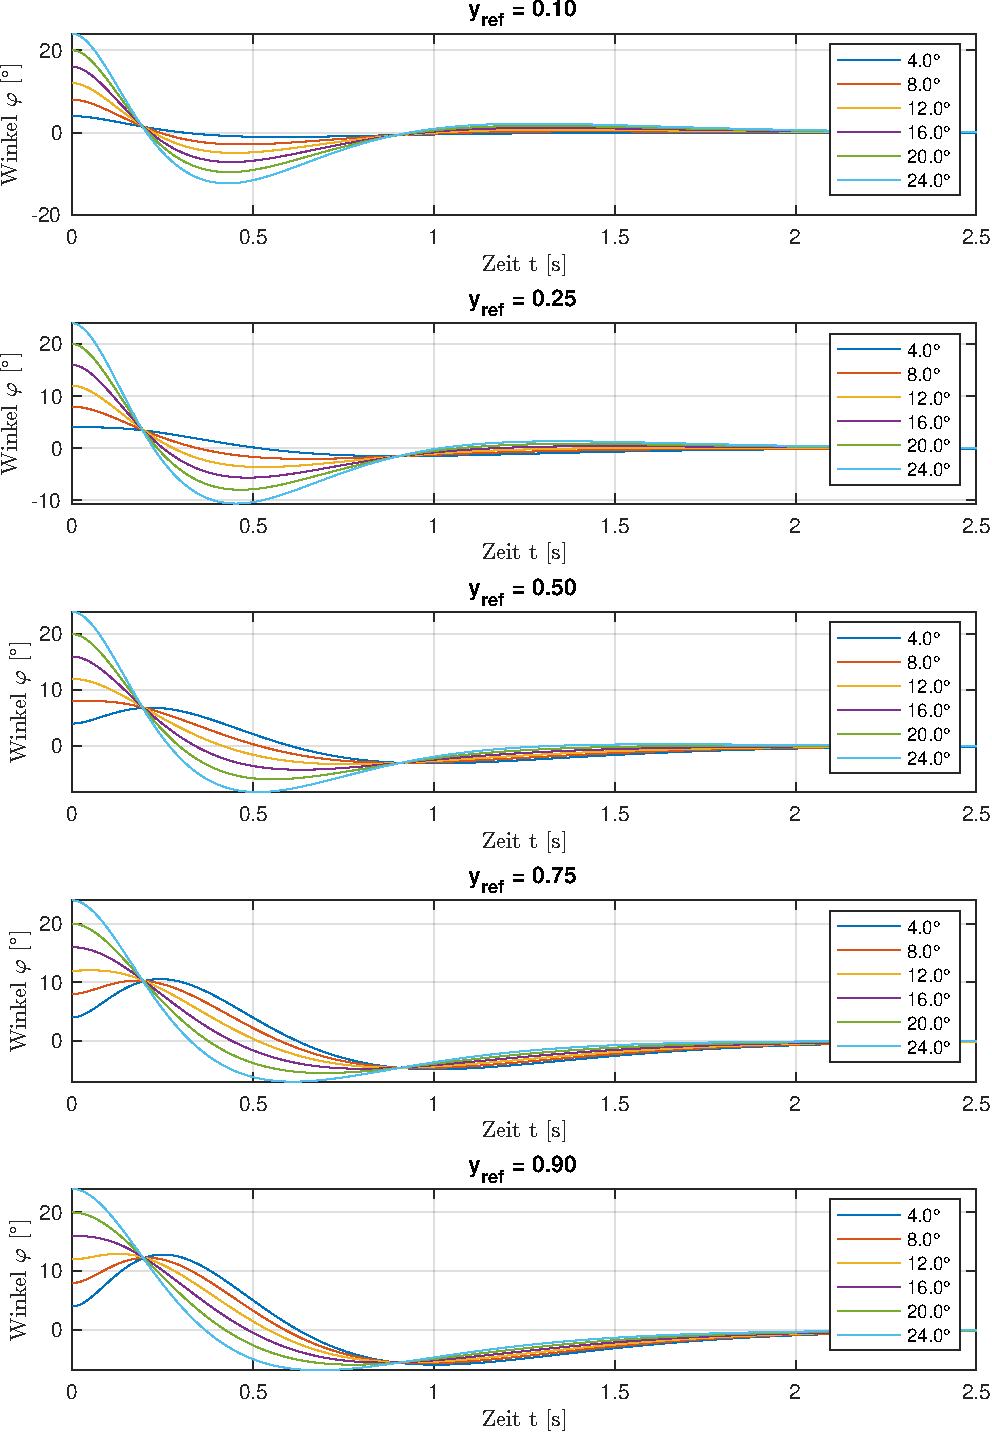
\includegraphics[width=0.8\textwidth]{Bilder/Reglervalidierung/nichtlinear_vorsteuerung_phi.pdf}}
    \caption[$\varphi$ für Regler mit Vorsteuerung (nichtlinear)]{$\varphi$ für verschiedene Referenzpositionen $y_{ref}$ und Anfangsauslenkungen am Zustandsregler mit Vorsteuerung für das nichtlineare Zustandsraummodell}
    \label{fig:Bild33}
\end{figure}

\begin{figure}[H]
    \centering
    \fbox{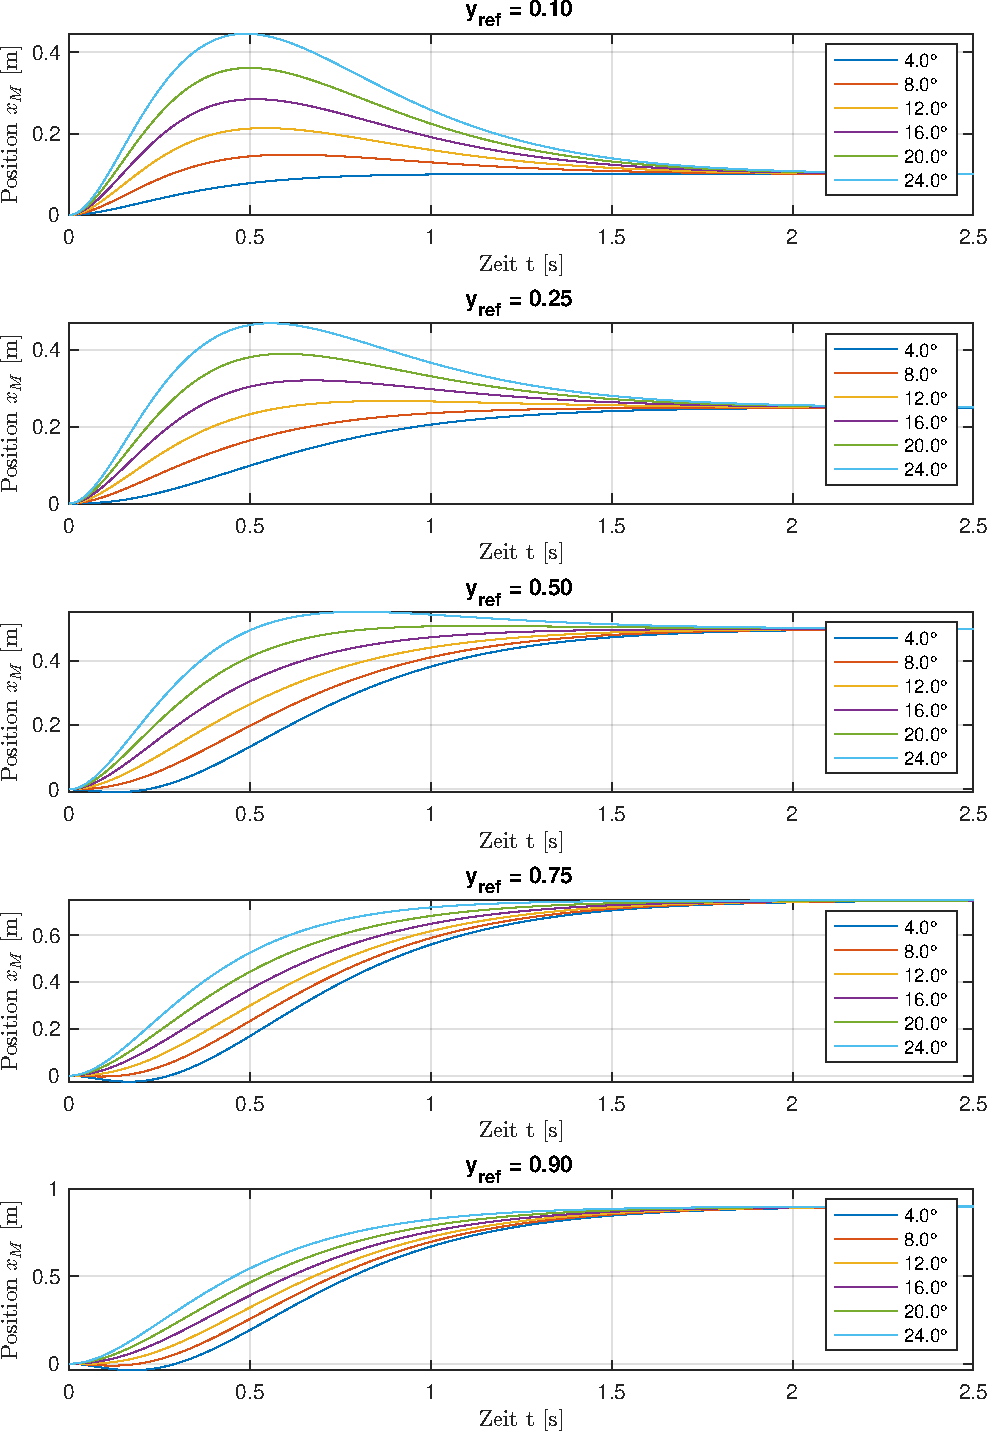
\includegraphics[width=0.8\textwidth]{Bilder/Reglervalidierung/nichtlinear_vorsteuerung_xM.pdf}}
    \caption[$x_{\mathrm{M}}$ für Regler mit Vorsteuerung (nichtlinear)]{$x_{\mathrm{M}}$ für verschiedene Referenzpositionen $y_{ref}$ und Anfangsauslenkungen am Zustandsregler mit Vorsteuerung für das nichtlineare Zustandsraummodell}
    \label{fig:Bild34}
\end{figure}

\begin{figure}[H]
    \centering
    \fbox{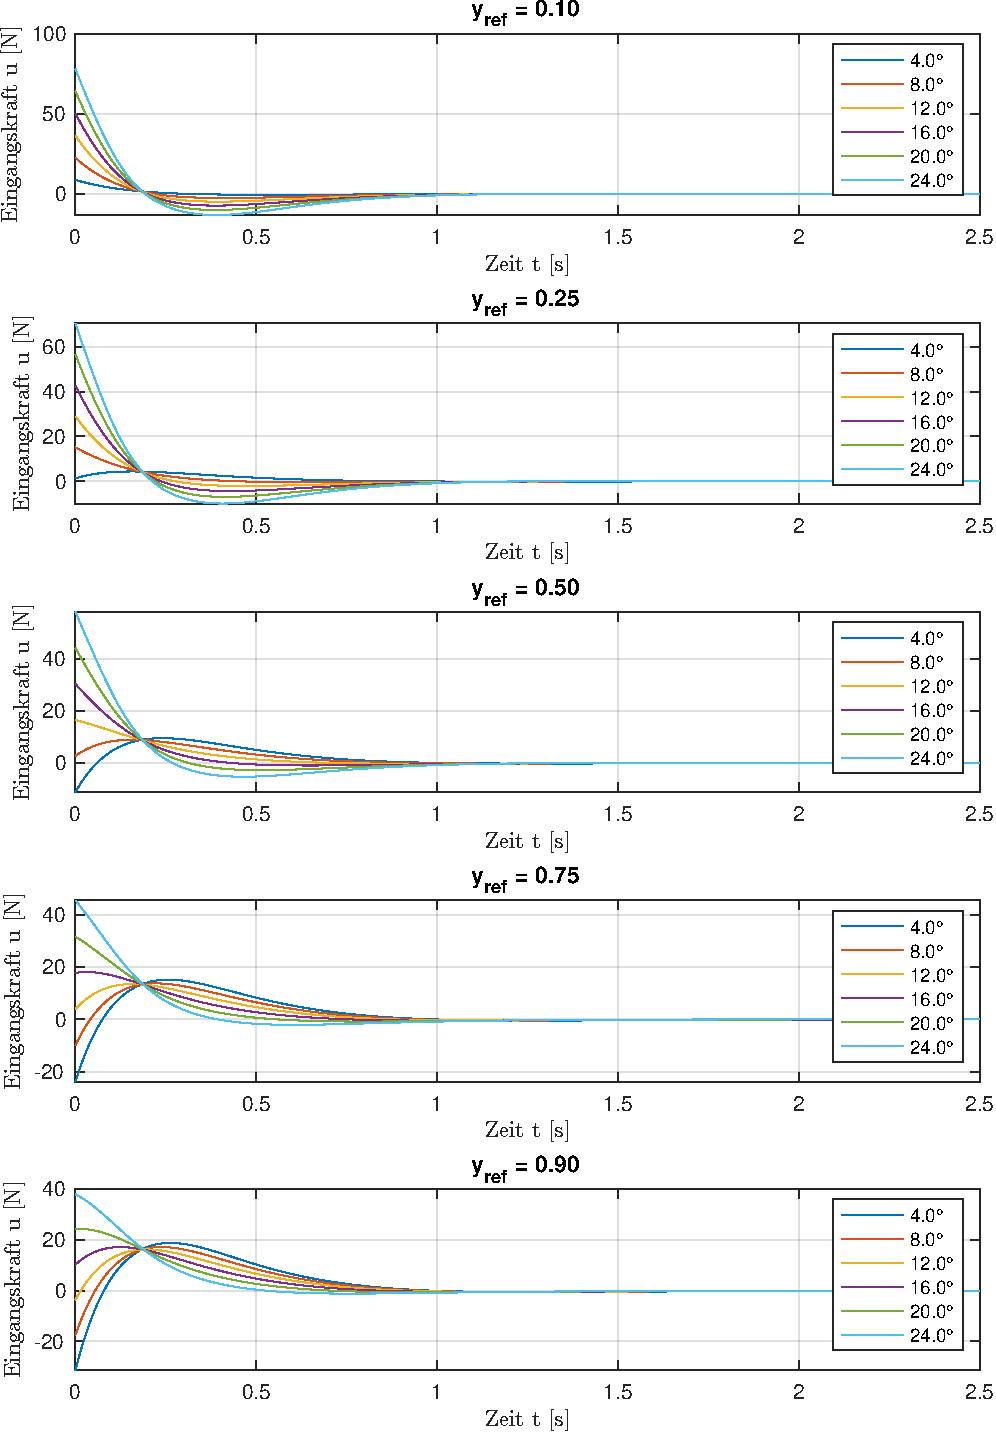
\includegraphics[width=0.8\textwidth]{Bilder/Reglervalidierung/nichtlinear_vorsteuerung_u.pdf}}
    \caption[u für Regler mit Vorsteuerung (nichtlinear)]{u für verschiedene Referenzpositionen $y_{ref}$ und Anfangsauslenkungen am Zustandsregler mit Vorsteuerung für das nichtlineare Zustandsraummodell}
    \label{fig:Bild35}
\end{figure}

\subsubsection{Zustandsregler mit I-Regelung}

\begin{figure}[H]
    \centering
    \fbox{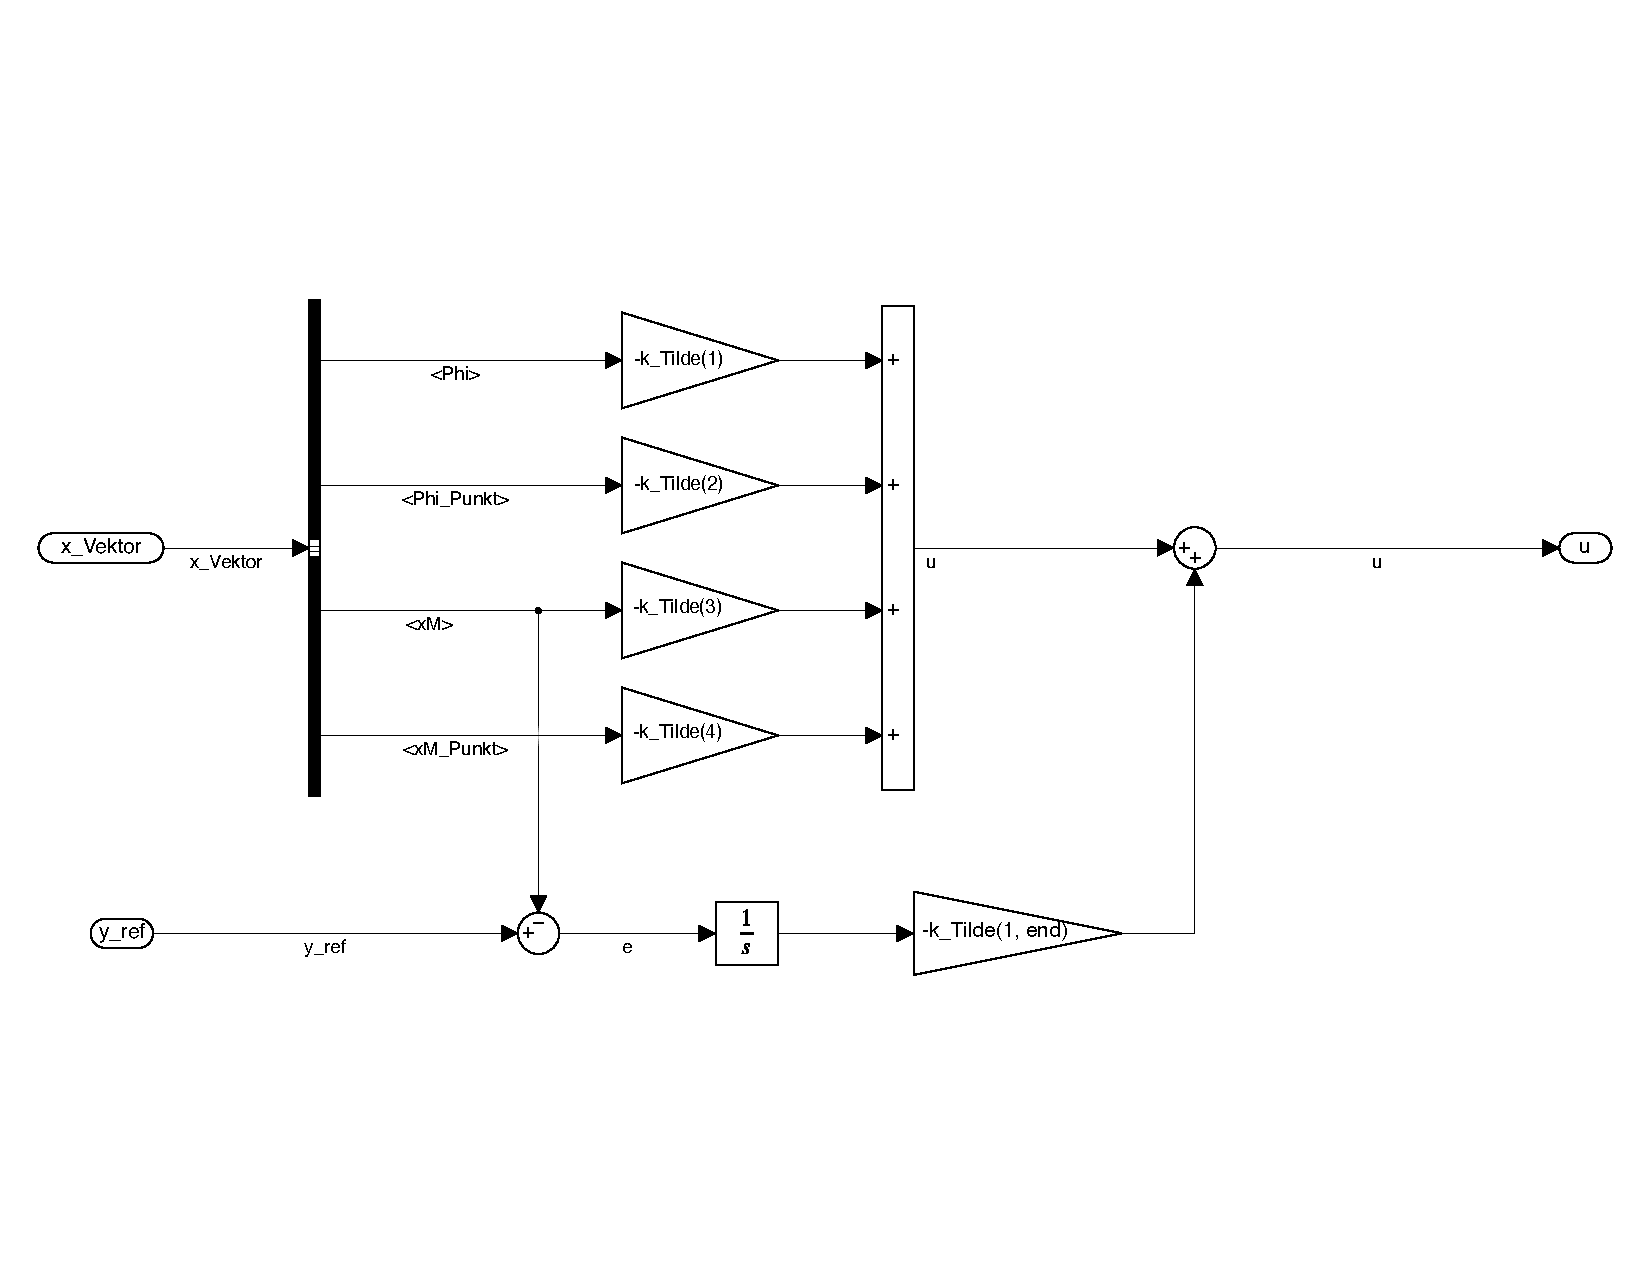
\includegraphics[width=1.0\textwidth]{Bilder/Reglervalidierung/I_Regler_nl.pdf}}
    \caption[Regler mit I-Regelung Simulink (nichtlinear)]{Simulink Regler-Blockschaltbild für den Zustandsregler mit I-Regelung (nichtlineares Zustandsraummodell)}
    \label{fig:Bild36}
\end{figure}

\begin{figure}[H]
    \centering
    \fbox{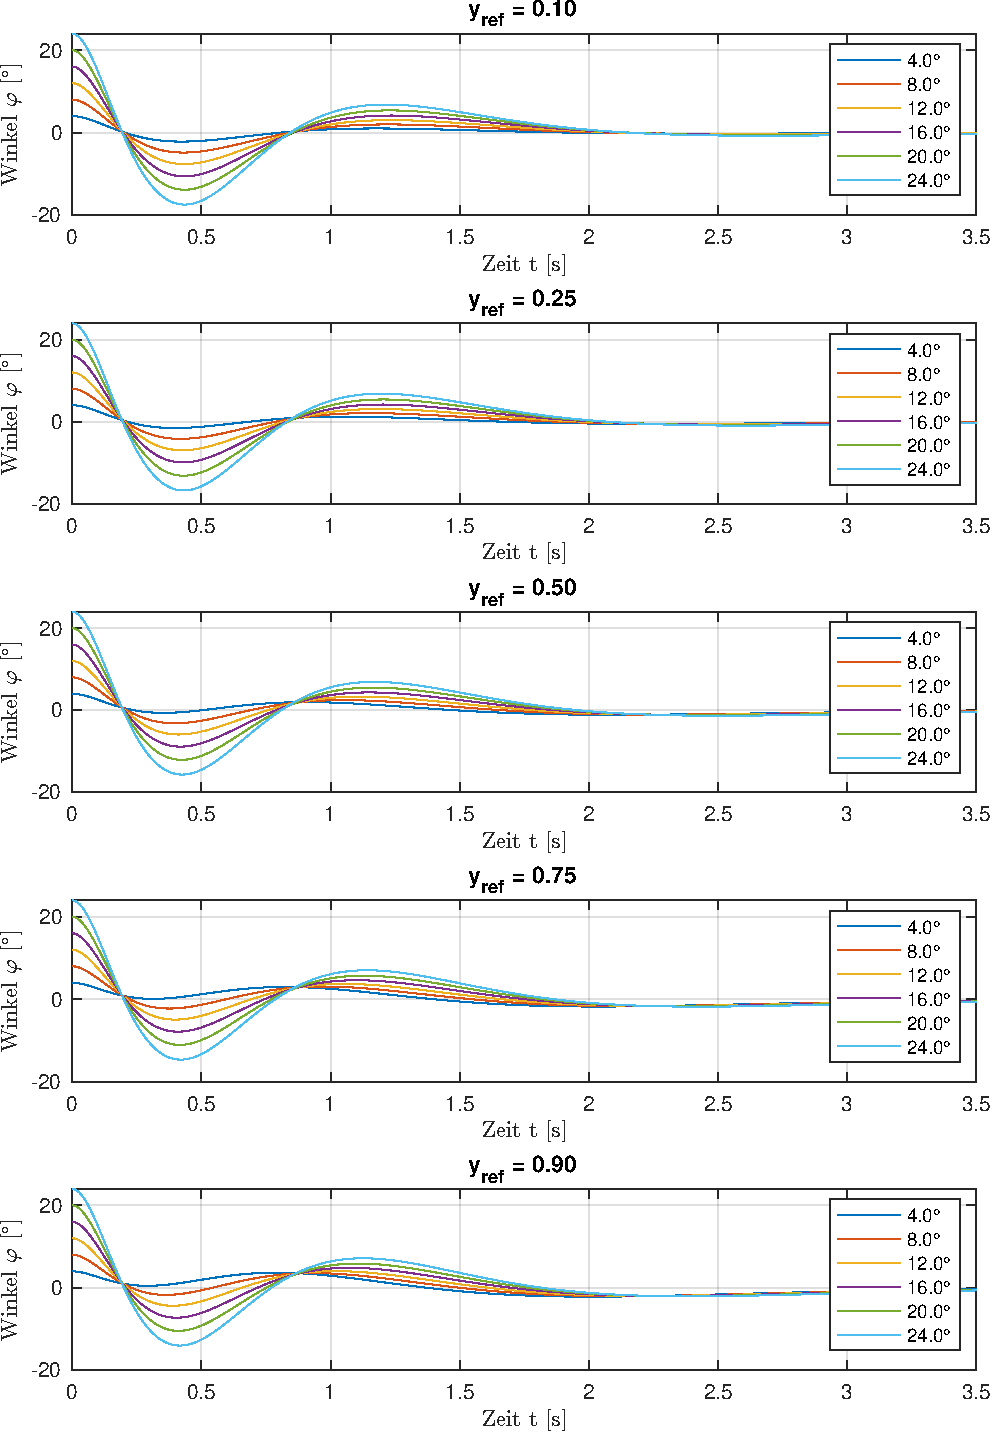
\includegraphics[width=0.8\textwidth]{Bilder/Reglervalidierung/nichtlinear_i_regler_phi.pdf}}
    \caption[$\varphi$ für Regler mit I-Regelung (nichtlinear)]{$\varphi$ für verschiedene Referenzpositionen $y_{ref}$ und Anfangsauslenkungen am Zustandsregler mit I-Regelung für das nichtlineare Zustandsraummodell}
    \label{fig:Bild37}
\end{figure}

\begin{figure}[H]
    \centering
    \fbox{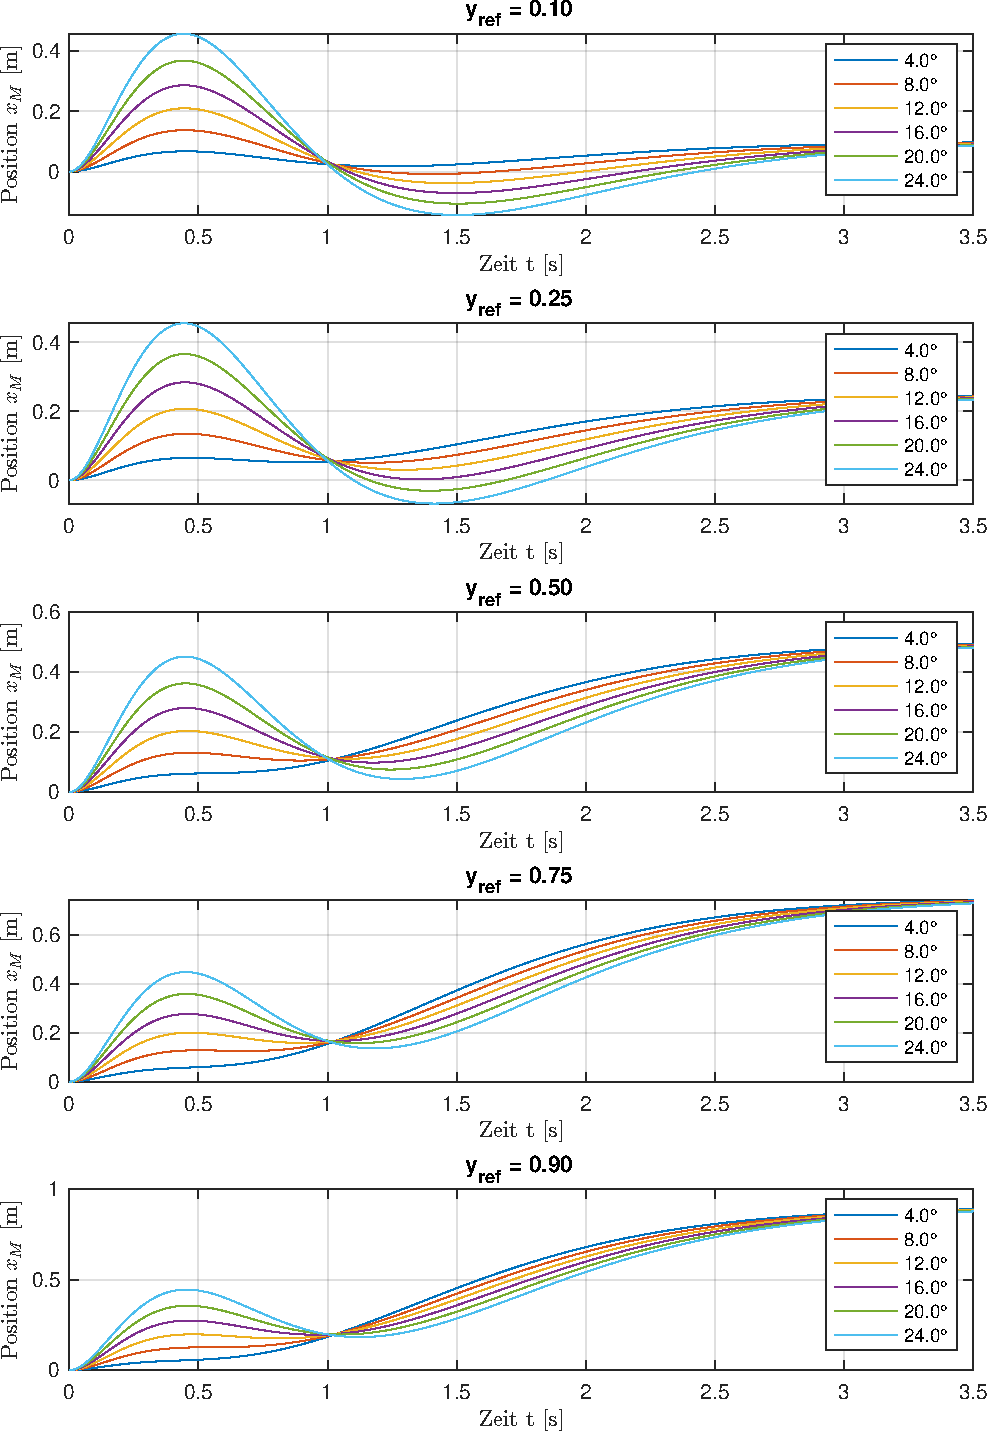
\includegraphics[width=0.8\textwidth]{Bilder/Reglervalidierung/nichtlinear_i_regler_xM.pdf}}
    \caption[$x_{\mathrm{M}}$ für Regler mit I-Regelung (nichtlinear)]{$x_{\mathrm{M}}$ für verschiedene Referenzpositionen $y_{ref}$ und Anfangsauslenkungen am Zustandsregler mit I-Regelung für das nichtlineare Zustandsraummodell}
    \label{fig:Bild38}
\end{figure}

\begin{figure}[H]
    \centering
    \fbox{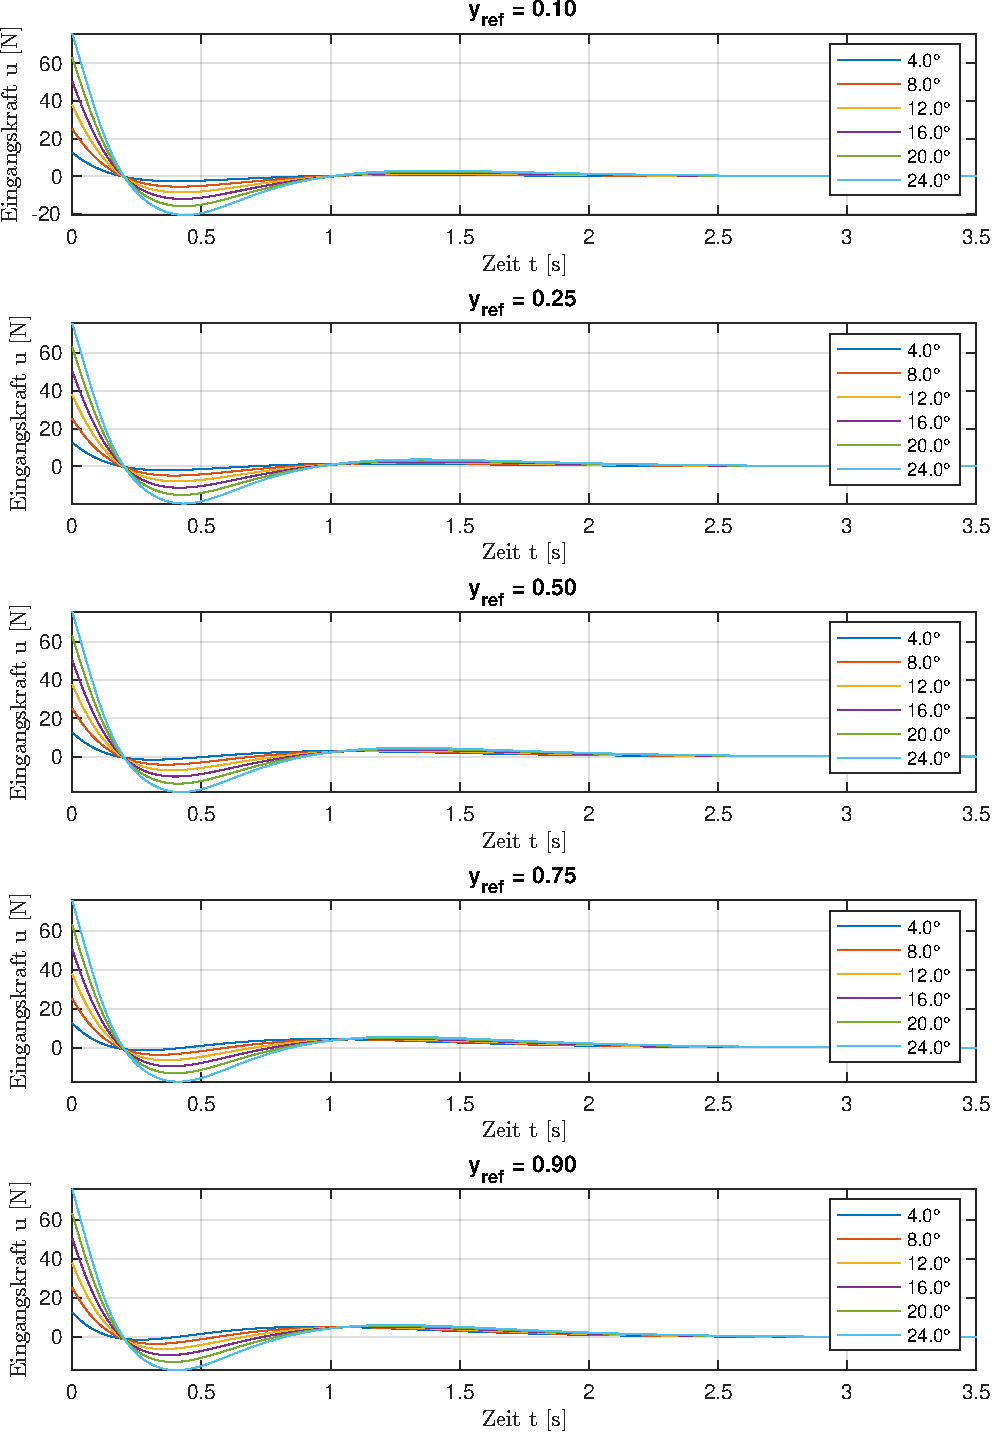
\includegraphics[width=0.8\textwidth]{Bilder/Reglervalidierung/nichtlinear_i_regler_u.pdf}}
    \caption[u für Regler mit I-Regelung (nichtlinear)]{u für verschiedene Referenzpositionen $y_{ref}$ und Anfangsauslenkungen am Zustandsregler mit I-Regelung für das nichtlineare Zustandsraummodell}
    \label{fig:Bild39}
\end{figure}

\subsubsection{Vergleich des Regelverhaltens}

\begin{figure}[H]
    \centering
    \fbox{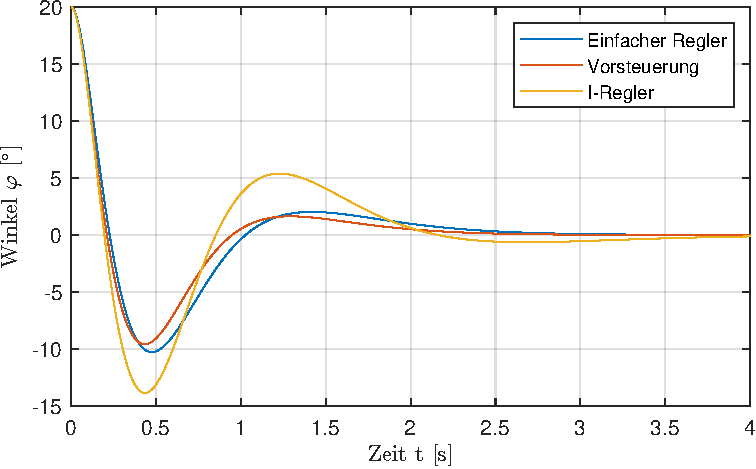
\includegraphics[width=0.65\textwidth]{Bilder/Reglervalidierung/nichtlinear_vergleich_phi.pdf}}
    \caption[Reglervergleich für $\varphi$ (nichtlinear)]{$\varphi$ für Regler mit einfacher Zustandsrückführung, Regler mit Vorsteuerung und Regler mit I-Regelung bei einer Anfangsauslenkungen von $20^\circ$ und einer Referenzposition $y_{ref} = 0,1 m$ am nichtlinearen Zustandsraummodell}
    \label{fig:Bild40}
\end{figure}

\begin{figure}[H]
    \centering
    \fbox{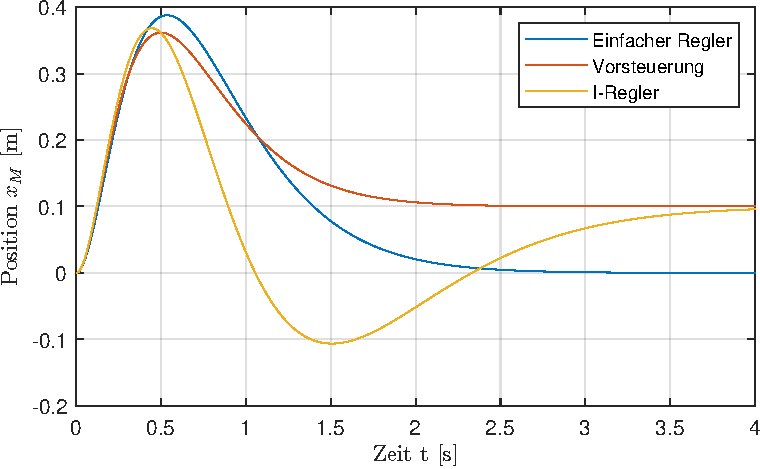
\includegraphics[width=0.65\textwidth]{Bilder/Reglervalidierung/nichtlinear_vergleich_xM.pdf}}
    \caption[Reglervergleich für $x_{\mathrm{M}}$ (nichtlinear)]{$x_{\mathrm{M}}$ für Regler mit einfacher Zustandsrückführung, Regler mit Vorsteuerung und Regler mit I-Regelung bei einer Anfangsauslenkungen von $20^\circ$ und einer Referenzposition $y_{ref} = 0,1 m$ am nichtlinearen Zustandsraummodell}
    \label{fig:Bild41}
\end{figure}

\begin{figure}[H]
    \centering
    \fbox{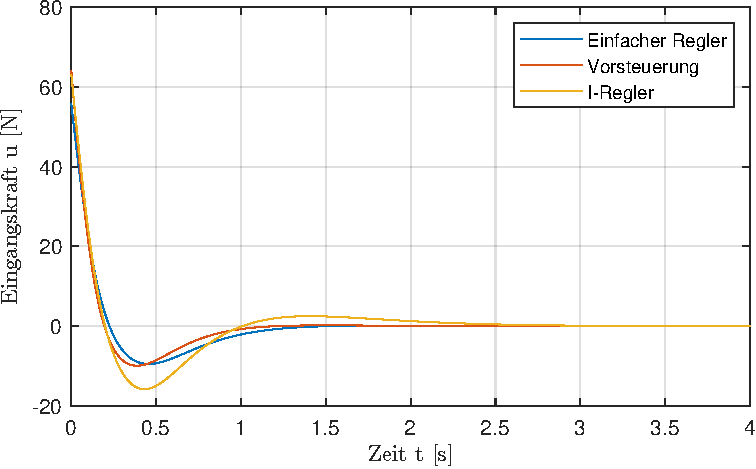
\includegraphics[width=0.65\textwidth]{Bilder/Reglervalidierung/nichtlinear_vergleich_u.pdf}}
    \caption[Reglervergleich für $u$ (nichtlinear)]{$u$ für Regler mit einfacher Zustandsrückführung, Regler mit Vorsteuerung und Regler mit I-Regelung bei einer Anfangsauslenkungen von $20^\circ$ und einer Referenzposition $y_{ref} = 0,1 m$ am nichtlinearen Zustandsraummodell}
    \label{fig:Bild42}
\end{figure}

\section{Beobachter}

Bisher wurde von einer wesentlichen Vereinfachung der Realität ausgegangen. Nämlich dass für Stabilisierung, Zustandsrückführung \etc der gesamte Zustandsvektor des Kontrollsystems zur Verfügung steht. Tatsächlich sind in der Regel nicht alle Zustandsinformationen bekannt. Beispielsweise weil sie technisch überhaupt nicht messbar sind oder nur unter großem technischen beziehungsweise finanziellen Aufwand ermittelt werden könnten. Sprachlich wird
vereinfacht gesagt, dass die entsprechenden Größen \textit{nicht messbar} sind.

\begin{align*}
    dim(y) < dim(x)
\end{align*}

\begin{figure}[H]
    \centering
    \fbox{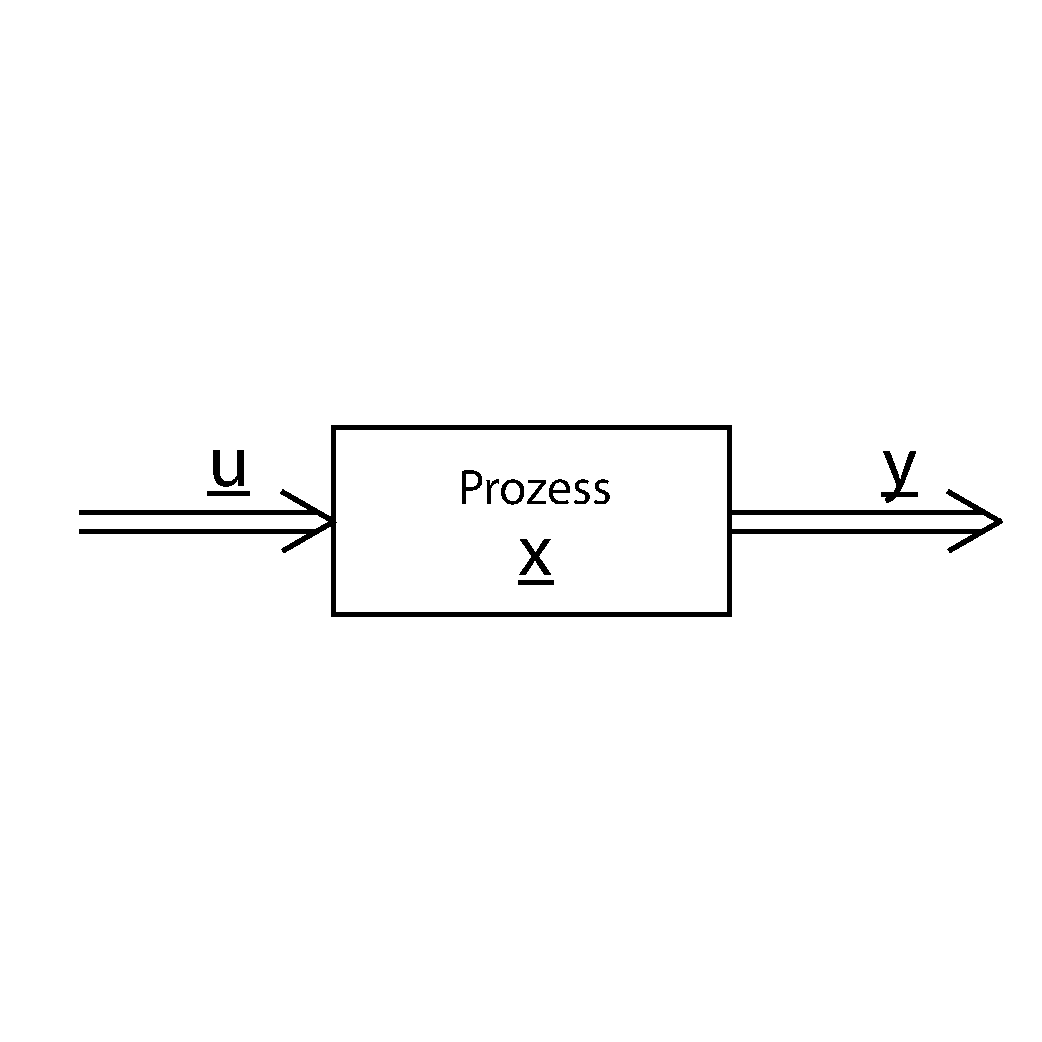
\includegraphics[width=0.5\textwidth]{Bilder/Beobachter/System.pdf}}
    \caption[Allgemeines System im Zustandsraum]{Schematische Darstellung eines allgemeinen Systems im Zustandsraum}
    \label{fig:Bild43}
\end{figure}

Da aber dennoch alle Zustände für die Zustandsregelung benötigt werden, wird der Beobachter eingeführt.\\
Mit dessen Hilfe ist es möglich innere Zustände zu rekonstruieren. Dies erfolgt über ein \textbf{Modell} und dem \textbf{Vergleich} der rekonstruierten Zustände mit den gemessenen Ausgängen (\autoref{fig:Bild44}).\\
\newline
Ansatz von Luenberger:
\[
    \underline{\dot{\hat{x}}} = 
    \underbrace{% 
        \underline{A} \cdot \underline{\hat{x}} + \underline{B} \cdot \underline{u}
    }_{%
    Modell
    }
    + 
    \underbrace{%
    \underline{L} \cdot\left( \underline{y} - \underline{\hat{y}}\right)
    }_{%
    Vergleich
    }
\]
\[
    \underline{\hat{y}} = \underline{C} \cdot \underline{\hat{x}}
\]
\newline
Im Fall des behandelten inversen Pendels kann die Winkelgeschwindigkeit $\dot{\varphi}$ nicht gemessen werden, sondern muss über den Beobachter rekonstruiert werden. Der mathematische Ansatz und die Umsetzung in Matlab/Simulink sind in den beiden folgenden Unterabschnitten beschrieben.

\begin{figure}[H]
    \centering
    \fbox{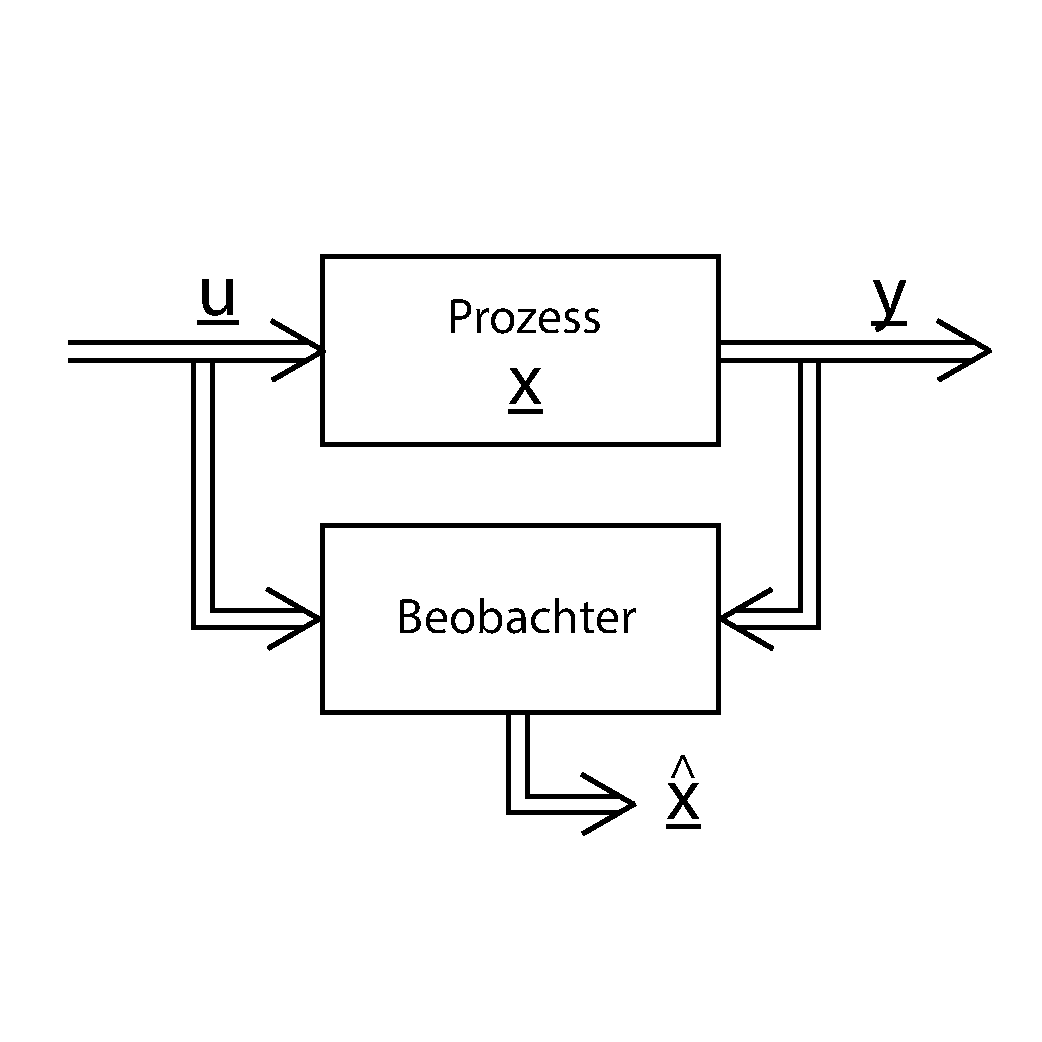
\includegraphics[width=0.5\textwidth]{Bilder/Beobachter/System_Beobachter.pdf}}
    \caption[System mit Beobachter]{Schematische Darstellung eines allgemeinen Systems mit Beobachter im Zustandsraum}
    \label{fig:Bild44}
\end{figure}

\subsection{Überprüfung der Beobachtbarkeit}

Naheliegend ist zunächst die Überlegung anzustellen, wann sich der Gesamtzustand $\underline{x}$ aus dem Ausgang $\underline{y}$ rekonstruieren lässt. Dies wird auch \textbf{Beobachtbarkeit} des Systems genannt. Konkret gilt der Satz: \\
\newline
\textit{Ein System ist beobachtbar, falls mit der Messung von $\underline{u}$ und $\underline{y}$ nach endlicher Zeit $t$ der unbekannte Zustandsvektor $\underline{x}$ vom System rekonstruiert werden kann.} \\
\newline
Der Beobachter lässt sich auf die Klasse der linearen zeitinvarianten Systeme (LTI) anwenden:
\begin{align}
    \underline{\dot{\hat{x}}} = \underline{A} \cdot \underline{\hat{x}} + \underline{B} \cdot \underline{u} + \underline{L} \cdot\left( \underline{y} - C \cdot \underline{\hat{x}}\right)
\end{align}
\newline
Ein System ist vollständig beobachtbar, falls für die Beobachtbarkeitsmatrix
\begin{align}
    Q_{\mathrm{Obs}} =
    \begin{pmatrix}
        \underline{C} \\
        \underline{C} \cdot \underline{A} \\
        \vdots \\
        \underline{C} \cdot \underline{A}^{n - 1}
    \end{pmatrix}
\end{align}
\newline
mit $n\in\mathbb{N}$, $p\in\mathbb{N}$, $A\in\mathbb{R}^{(n\times n)}$, $C\in\mathbb{R}^{(p\times n)}$ für SISO Systeme
\begin{align}
    det(Q_{\mathrm{Obs}}) \neq 0
\end{align}
und für MIMO \bzw SIMO Systeme
\begin{align}
    rank(Q_{\mathrm{Obs}}) = n \quad \text{\bzw} \quad m
\end{align}
\newline
gilt, wobei $n$ die Anzahl der linear unabhängigen Zeilen einer Matrix ist und $m$ die Anzahl der linear unabhängigen Spalten. Falls
\begin{align*}
    n &> m: \\
    rank(X) &= m
\end{align*}
\newline
und falls
\begin{align*}
    m &> n: \\
    rank(X) &= n.
\end{align*}
\newline
Die konkrete C-Matrix für das inverse Pendel
\begin{align}
    C_{\mathrm{Obs}} = 
    \begin{bmatrix}
        1 & 0 & 0 & 0 \\
        0 & 0 & 1 & 0 \\
        0 & 0 & 0 & 1
    \end{bmatrix}
\end{align}
\newline
besitzt p Zeilen, wobei sich die Anzahl der Zeilen nach den messbaren Zuständen richtet. Zu erkennen ist, dass ein SIMO System auf Beobachtbarkeit untersucht werden muss. Somit muss der Rang der Beobachtbarkeitsmatrix bestimmt werden.\\
Das Aufstellen der Beobachtbarkeitsmatrix führt zu
\begin{align}
    Q_{\mathrm{Obs}} = 
    \begin{bmatrix}
        1 & 0 & 0 & 0 \\
        0 & 0 & 1 & 0 \\
        0 & 0 & 0 & 1 \\
        0 & 1 & 0 & 0 \\
        0 & 0 & 0 & 1 \\
        -0.8502 & 0.0008 & 0 & -2.3333 \\
       26.6505 & -0.0248 & 0 & 5.8333 \\
       -0.8502 & 0.0008 & 0 & -2.3333 \\
        2.0049 & -0.8521 & 0 & 5.4491 \\
       -5.6209 & 26.6557 & 0 & -13.7559 \\
        2.0049 & -0.8521 & 0 & 5.4491 \\
      -27.3408 & 2.0304 & 0 & -17.6849
    \end{bmatrix}.
\end{align}

Der Rang folgt zu:
\begin{align}
    rank(Q_{\mathrm{Obs}}) = 4
\end{align}
\newline
Da $n > m$ muss $rank(Q_{\mathrm{Obs}}) = 4$ gelten. Da dies der Fall ist, ist das System beobachtbar.

\subsection{Beobachterentwurf}

Wie bereits bei der Untersuchung der Beobachtbarkeit festgestellt wurde, handelt es sich bei dem zu beobachtenden System um ein SIMO System. Im Folgenden soll der Beobachter auf einen Zustandsregler mit I-Regelung (wie bereits in \autoref{sec:iregler} mit Referenzwertvorgabe für $x_{\mathrm{M}}$) angewendet werden. Damit der Beobachter auf diesen Regler angewendet werden kann, muss dieser zunächst implementiert werden. Dazu müssen bevor der Beobachterentwurf stattfinden kann, zunächst passende k-Faktoren über die Formulierung von linearen Matrixungleichungen gefunden werden. Als Ansatz gelten die \textbf{Quadratischen Ljapunov Funktionen}:
\begin{align}
    V(\underline{x}) = \underline{x}^T \cdot \underline{P} \cdot \underline{x} \\
    V(\underline{x}) > \underline{0} \curvearrowright   \underline{P} > \underline{0} \quad mit \quad 
    \underline{P} = \underline{P}^T \nonumber
\end{align}
\newline
Die zeitliche Ableitung der Funktion folgt zu:
\begin{align}
    \dot{V}(\underline{x}) &= \dot{\underline{x}}^T \cdot \underline{P} \cdot \underline{x} + \underline{x}^T \cdot \underline{P} \cdot \dot{\underline{x}}
\end{align}
\newline
mit $\dot{\underline{x}} = (\underline{A}-\underline{B}\cdot\underline{k})\cdot\underline{x}$:
\begin{align}
    \dot{V}(\underline{x}) &= ((\underline{A}-\underline{B}\cdot\underline{k})\cdot\underline{x})^T \cdot \underline{P} \cdot \underline{x} + \underline{x}^T \cdot \underline{P} \cdot (\underline{A}-\underline{B}\cdot\underline{k})\cdot\underline{x} \nonumber \\
    \dot{V}(\underline{x}) &= \underline{x}^T\cdot(\underline{A}^T\cdot\underline{P}-\underline{k}^T\cdot\underline{B}^T\cdot\underline{P}+\underline{P}\cdot\underline{A}-\underline{P}\cdot\underline{B}\cdot\underline{k})\cdot\underline{x}
\end{align}
\newline
Gewählt wurde weiterhin der Ansatz für exponentielle Stabilität. Gesucht ist somit
\begin{align}
    \dot{V}(\underline{x}) < -2\cdot\alpha \cdot V(\underline{x})
\end{align}
\newline
mit $\alpha > 0$ als als vorgegebene Abklingrate (Decay-Rate).\\

\clearpage

Mit dem Kriterium für exponentielle Stabilität folgt:
\[
    \underbrace{% 
        \underline{x}^T\cdot(\underline{A}^T\cdot\underline{P}-\underline{k}^T\cdot\underline{B}^T\cdot\underline{P}+\underline{P}\cdot\underline{A}-\underline{P}\cdot\underline{B}\cdot\underline{k})\cdot\underline{x}
    }_{%
    \dot{V}(\underline{x})
    }
    < 
    \underbrace{%
    -2\cdot\alpha \cdot \underline{x}^T\cdot\underline{P}\cdot\underline{x}
    }_{%
    -2\cdot\alpha\cdot V(\underline{x})
    }
\]

\begin{align} \label{eq:Gleichung82}
     \underline{x}^T\cdot(\underline{A}^T\cdot\underline{P}-\underline{k}^T\cdot\underline{B}^T\cdot\underline{P}+\underline{P}\cdot\underline{A}-\underline{P}\cdot\underline{B}\cdot\underline{k}+2\cdot\alpha\cdot\underline{P})\cdot\underline{x} < \underline{0}
\end{align}
\newline
Dies ist erfüllt, falls die zusammengesetzte Matrix negativ definit ist, also 
\begin{align*}
     \underline{A}^T\cdot\underline{P}-\underline{k}^T\cdot\underline{B}^T\cdot\underline{P}+\underline{P}\cdot\underline{A}-\underline{P}\cdot\underline{B}\cdot\underline{k}+2\cdot\alpha\cdot\underline{P} < \underline{0}
\end{align*}
\newline
gilt.\\
\newline
Die \autoref{eq:Gleichung82} enthält nichtlineare Terme. Zur Überführung in eine lineare Gleichung wird eine Variable $\underline{M}=\underline{k}\cdot\underline{x}$ eingeführt.
\begin{align} \label{eq:Gleichung83}
    \underline{x}\cdot\underline{A}^T+\underline{A}\cdot\underline{x}-\underline{M}^T\cdot\underline{B}^T-\underline{B}\cdot\underline{M}+2\cdot\alpha\cdot\underline{x} < \underline{0} \\
    \underline{x} > \underline{0} \nonumber
\end{align}
\newline
Analog zu \autoref{sec:iregler} wird die Matrix C wie folgt gewählt:
\begin{align*}
    C = 
    \begin{bmatrix}
        0 & 0 & 1 & 0
    \end{bmatrix}
\end{align*}
\newline
Ebenfalls müssen wieder $\underline{\tilde{A}}$ und $\underline{\tilde{B}}$ bestimmt werden:
\begin{align*}
    \underline{\tilde{A}} &= 
    \begin{bmatrix}
        \underline{A} & \underline{0} \\
        -\underline{C} & \underline{0}
    \end{bmatrix} \quad ; \underline{\tilde{A}}\in\mathbb{R}^{(n+p)x(n+p)}\\
    \underline{\tilde{B}} &= 
    \begin{bmatrix}
        \underline{B} \\
        \underline{0}
    \end{bmatrix}\qquad ; \underline{\tilde{B}}\in\mathbb{R}^{(n+p)x(m)}
\end{align*}
\newline
Zuletzt wird $\alpha$ gewählt zu
\begin{align*}
    \alpha = 0.6.
\end{align*}
\newline

Über die LMI-Funktionen in Matlab kann nun die lineare Matrixungleichung aus \autoref{eq:Gleichung83} gelöst werden.\\\\
Die $\tilde{k}$-Matrix mit $\underline{k} = \underline{M}\cdot\underline{x}^{-1}$ resultiert zu:
\begin{align}
    \underline{\tilde{k}} &= 
    \begin{bmatrix}
        -314.9301 & -58.3101 & -108.2878 & -84.0734 & 59.0425
    \end{bmatrix}
\end{align}
\newline
Gemäß \autoref{eq:Gleichung62} folgen die Verstärkungskoeffizienten wie nachfolgend gezeigt:\\\\
Zustandsrückführungskoeffizienten:
\begin{align}
    \underline{k}_{\mathrm{x}} &= 
    \begin{bmatrix}
        -314.9301 & -58.3101 & -108.2878 & -84.0734
    \end{bmatrix}
\end{align}
\newline
I-Verstärkungskoeffizienten:
\begin{align}
    \underline{k}_{\mathrm{I}} &= [-59.0425]
\end{align}
\newline
Die Polstellen des Reglers können abschließend berechnet werden über:
\begin{align}
    \begin{split}
        \underline{s}_{\mathrm{P}} &= eig(\underline{\tilde{A}} - \underline{\tilde{B}}\cdot\underline{\tilde{k}}) \\&=
        \begin{bmatrix}
            -9.4 + 5.1i & -9.4 - 5.1i & -1.2 + 0i & -1.5 + 1.2i & -1.5 - 1.2i
        \end{bmatrix}
    \end{split}
\end{align}

\begin{figure}[H]
    \centering
    \fbox{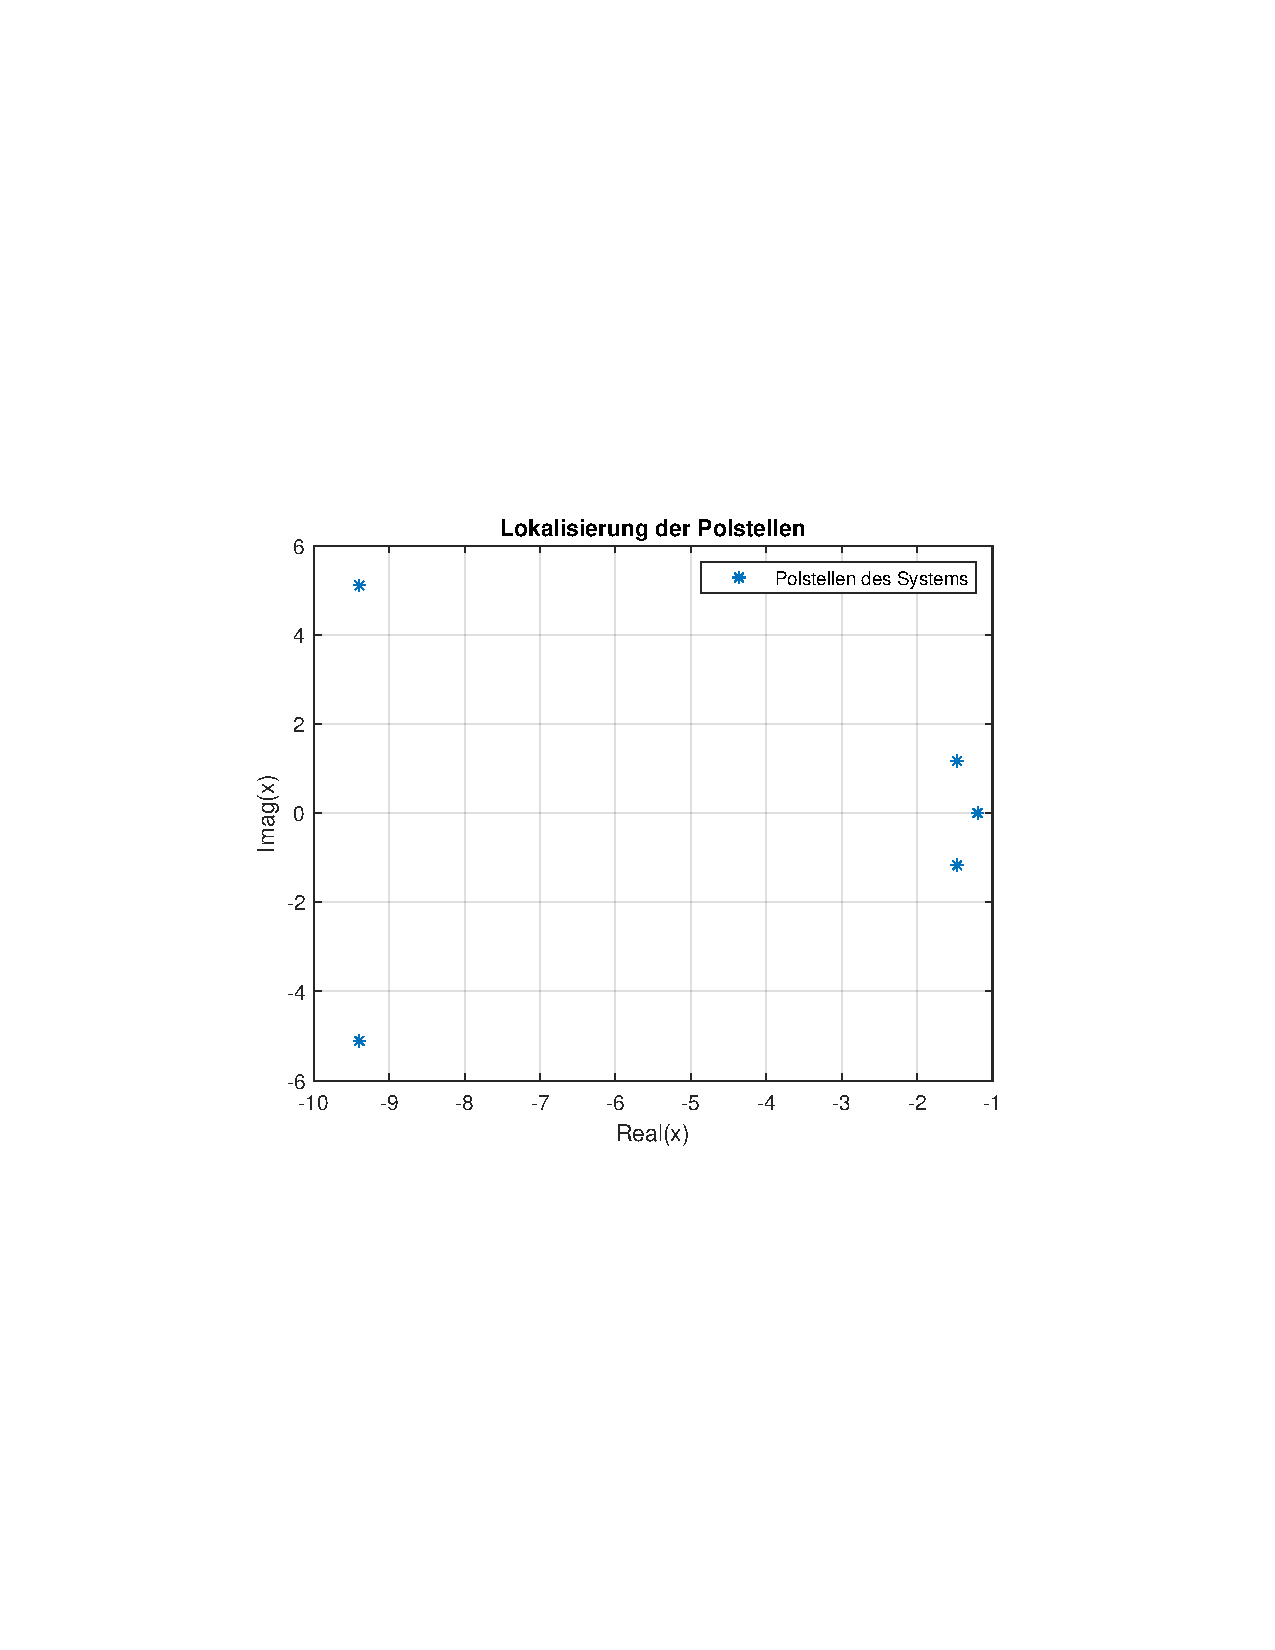
\includegraphics[width=0.75\textwidth]{Bilder/Polstellen_Regler_LMI.pdf}}
    \caption[Polstellen Regler mit LMI]{Polstellenlage des Systems mit I-Regelung und LMI}
    \label{fig:Bild45}
\end{figure}

Nachdem der Regler nun erfolgreich über LMI's implementiert wurde, kann nun mit dem Beobachterentwurf fortgesetzt werden.\\
Eine wichtige Erkenntnis wurde bis jetzt vorenthalten. zwischen dem Zustandsreglerentwurf und dem Beobachterentwurf besteht eine \textbf{Dualität}. Das heißt konkret, das erneut der Ansatz mit quadratischen Ljapunov-Funktionen angesetzt werden kann, um den Beobachter umzusetzen.
\begin{align}
    V(\underline{e}) = \underline{e}^T \cdot \underline{P} \cdot \underline{e} \quad mit \quad V(\underline{e}) > 0 \quad , \quad \underline{e} \neq 0 
\end{align}
\newline
Auch hier wird ein Beobachter mit Abklingrate gewählt, um diesmal einen exponentiellen Verlauf des Beobachterfehlers zu ermöglichen. Über $\alpha$ kann die Abklingrate des Fehlers genau eingestellt werden. Gesucht ist nun:
\begin{align}
    \dot{V}(\underline{e}) + 2 \cdot \alpha \cdot V(\underline{e}) < 0
\end{align}

\clearpage

Somit kann analog zum Regler eine LMI Formulierung mit $\underline{N}=\underline{P}\cdot\underline{L}$ vorgenommen werden. 
\begin{align} \label{eq:Gleichung90}
    \begin{split}
        \underline{A}^T\cdot\underline{P} + \underline{P}\cdot\underline{A} - \underline{N}\cdot\underline{C} - \underline{C}^T\cdot\underline{N} + 2\cdot\alpha\cdot\underline{P} < 0 \\
        \underline{P} > 0
    \end{split}
\end{align}
\newline
Zuletzt wird $\alpha$ gewählt zu
\begin{align*}
    \alpha _{Obs} = 4.0.
\end{align*}
\newline
Über die LMI-Funktionen in Matlab kann nun die lineare Matrixungleichung aus \autoref{eq:Gleichung90} gelöst werden.\\\\
Die L-Matrix mit $\underline{L} = \underline{P}^{-1}\cdot\underline{N}$ resultiert zu:
\begin{align}
    L &= 
    \begin{bmatrix}
        9.7627 & -0.1421 & 1.1786 \\
        72.8250 & -0.6596 & 11.3192 \\
        0.2876 & 4.5000 & 1.0417 \\
        -3.2221 & -0.0416 & 2.1657
    \end{bmatrix}
\end{align}
\newline
Die Polstellen des Beobachters können abschließend berechnet werden über:
\begin{align}
    \begin{split}
        \underline{s}_{\mathrm{P}} &= eig(\underline{A} - \underline{L}\cdot\underline{C}) \\&=
        \begin{bmatrix}
            -4.9 + 5.0i & -4.9 - 5.0i & -4.5 + 0.03i & -4.5 - 0.03i
        \end{bmatrix}
    \end{split}
\end{align}

\begin{figure}[H]
    \centering
    \fbox{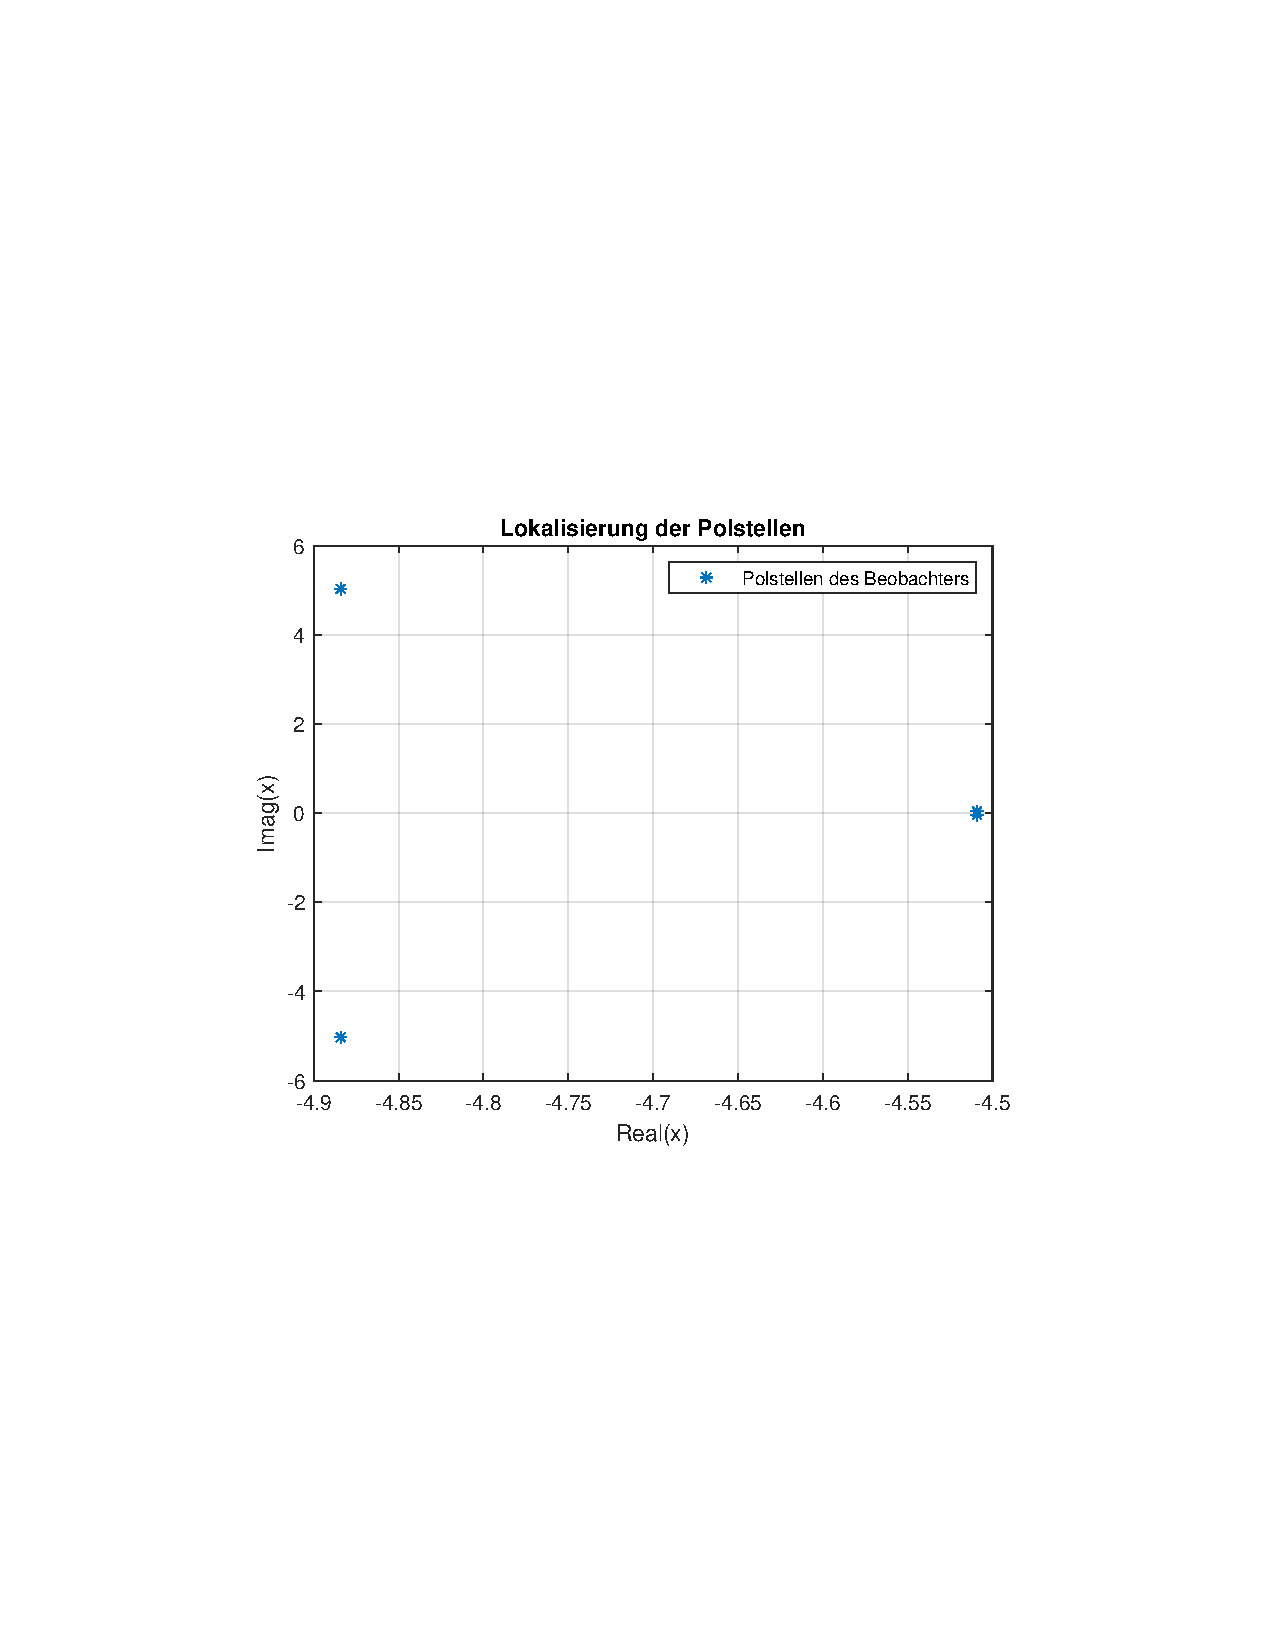
\includegraphics[width=0.75\textwidth]{Bilder/Polstellen_Beobachter_LMI.pdf}}
    \caption[Polstellen des Beobachters]{Polstellenlage des Beobachters}
    \label{fig:Bild46}
\end{figure}

Wichtig dabei ist zu beachten, dass das Systemverhalten des Beobachter schneller sein muss, als die des geschlossenen Regelkreises. Es gilt:
\begin{align}
    \left| Re\{ \underline{s}_{\mathrm{P}_{Obs}}\}\right| > \left| Re\{ \underline{s}_{\mathrm{P}_{Regler}}\}\right| \cdot (2 ... 3)
\end{align}
\newline
\autoref{fig:Bild47} zeigt die Systemstruktur des Zustandsreglers mit I-Regelung inklusive Beobachter.

\begin{figure}[H]
    \centering
    \fbox{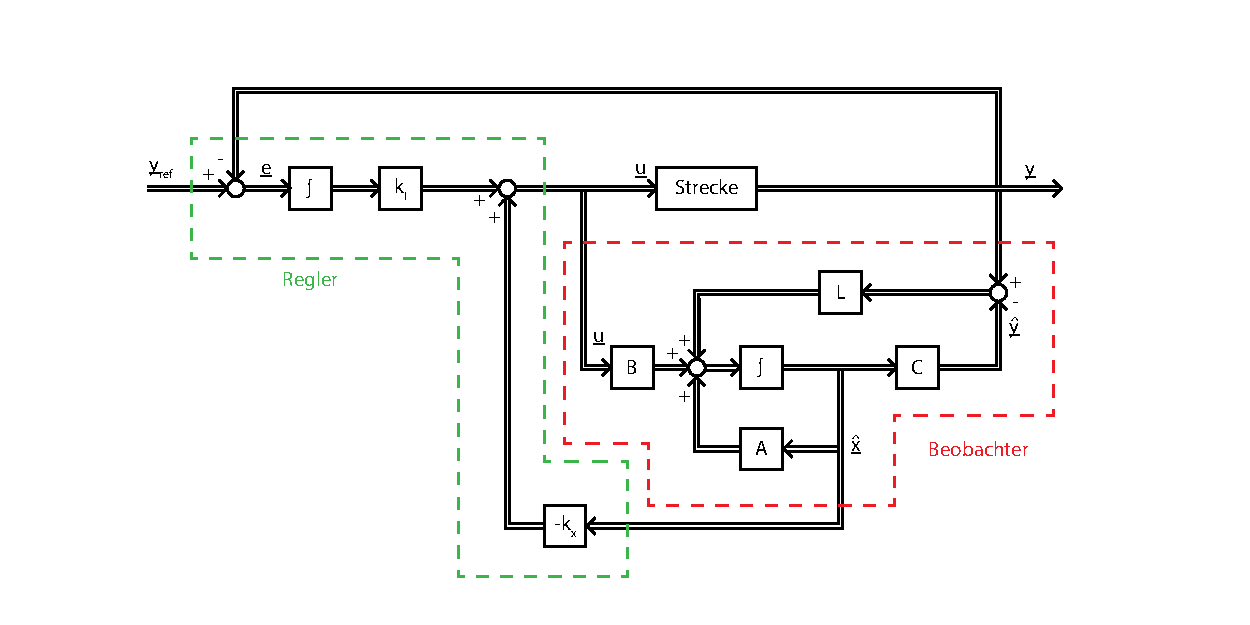
\includegraphics[width=1.0\textwidth]{Bilder/Beobachter/Beobachter_Regler_Strecke.pdf}}
    \caption[Reglerstruktur mit Beobachter]{Schematische Darstellung des Zustandsreglers mit I-Regelung und Beobachter}
    \label{fig:Bild47}
\end{figure}

\subsection{Beobachtervalidierung}

Im letzten Unterabschnitt der Arbeit soll der entwickelte Beobachter auf seine Funktionstüchtigkeit validiert werden. Wie bereits im vorangegangenen Abschnitt postuliert, wird der Beobachter auf den Zustandsregler mit I-Regelung angewendet. Das Modell in Simulink wird entsprechend des entworfenen Schemas in \autoref{fig:Bild47} umgesetzt. \autoref{fig:Bild48} zeigt die Blockstruktur des Beobachters, welcher mit in den Regelkreis integriert wurde. $\underline{\hat{x}}$ enthält die vier rekonstruierten Zustände des Systems. Unter anderem ist dort auch der Zustand $\dot{\varphi}$ wiederzufinden, der wie eingangs erwähnt nicht gemessen, sondern ausschließlich über den Beobachter ermittelt werden kann. \autoref{fig:Bild49} zeigt das Ergebnis der erfolgreichen Rekonstruktion der Winkelgeschwindigkeit des Pendels. Der Kurvenverlauf verhält sich ähnlich zum messbaren Winkel $\varphi$ des Systems. Weiterhin ist zu erkennen, dass die Winkelgeschwindigkeit wieder zu $0 m/s$ ausgeregelt wird, was ebenfalls plausibel ist, da das Pendel wieder in der Ruhelage verharrt, sobald eine Eingangsstörung (in diesem Fall eine Auslenkung von $20^\circ$) auf das System ausgeregelt wurde.

\begin{figure}[H]
    \centering
    \fbox{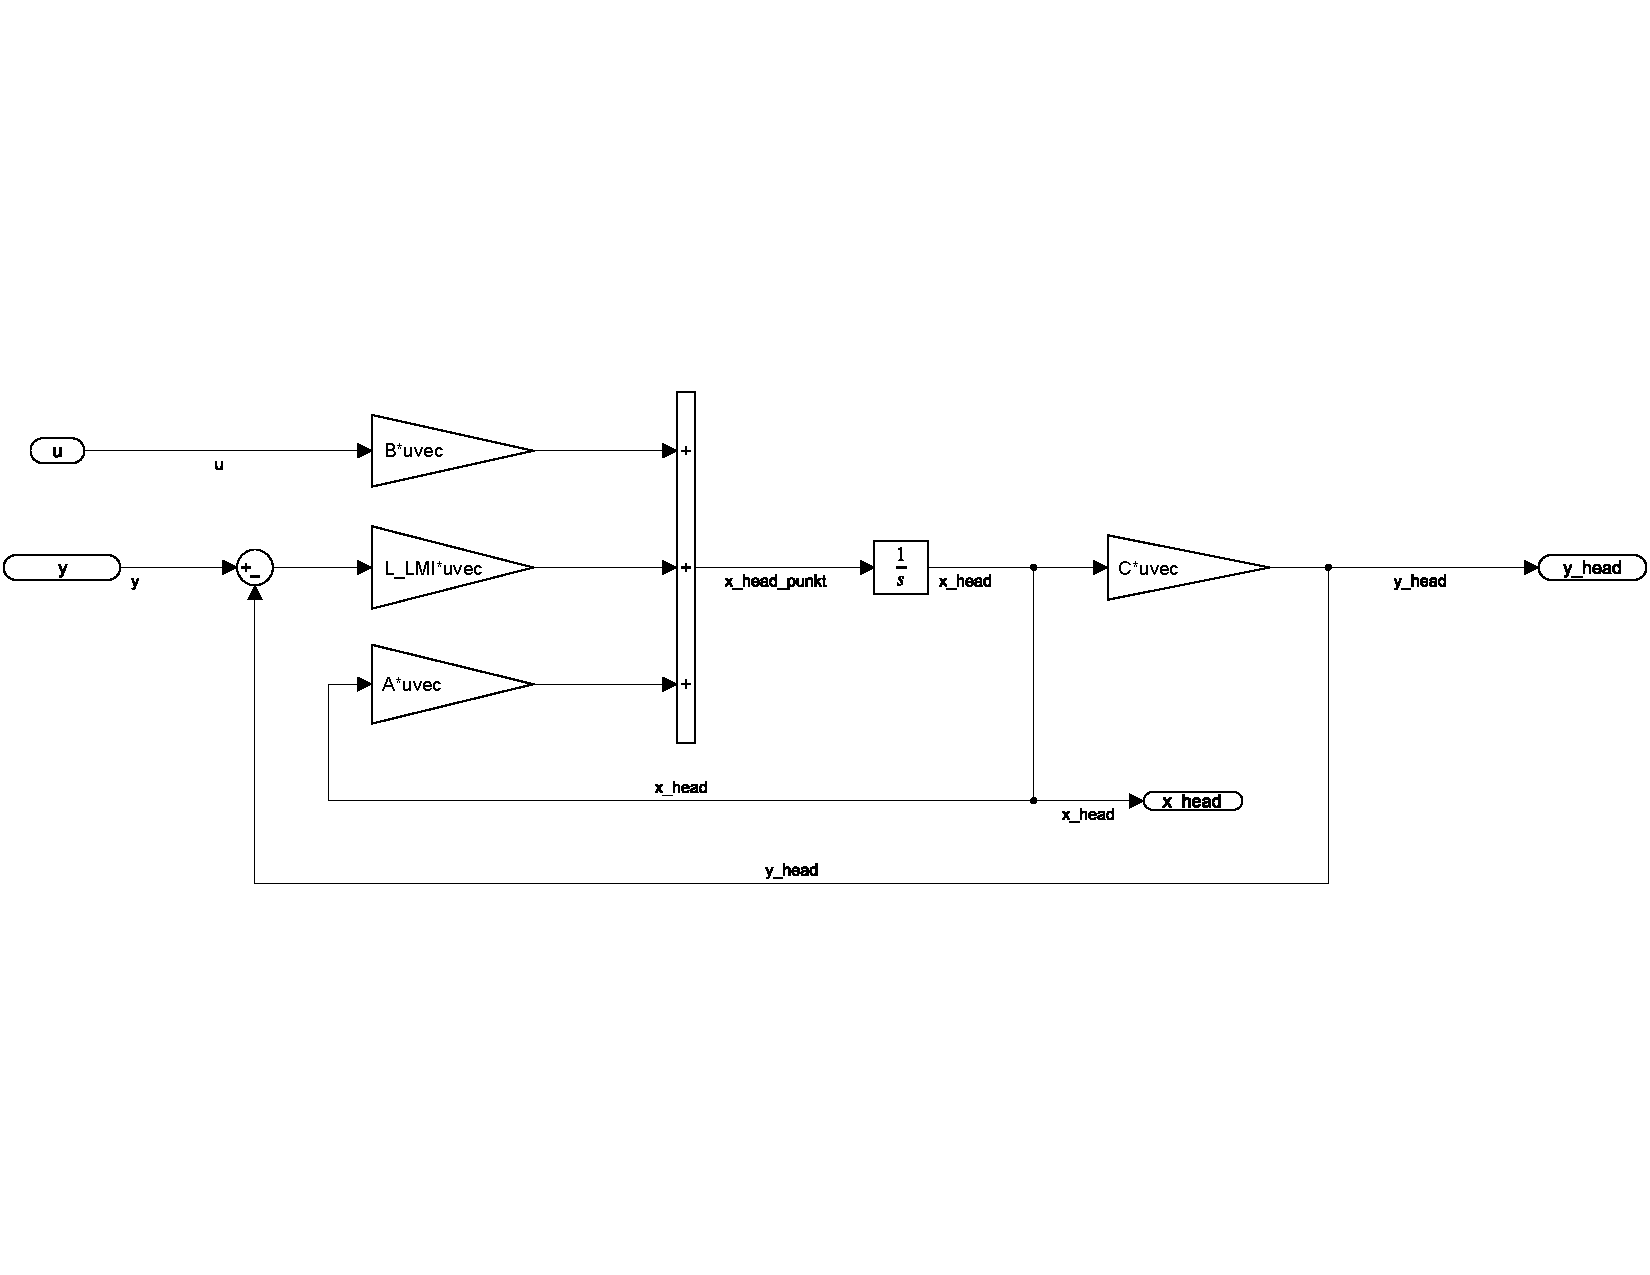
\includegraphics[width=1.0\textwidth]{Bilder/Beobachter/Simulink_Beobachter.pdf}}
    \caption[Beobachter Simulink]{Simulink Beobachter-Blockschaltbild für Zustandsregler mit I-Regelung und LMI}
    \label{fig:Bild48}
\end{figure}

\begin{figure}[H]
    \centering
    \fbox{\includegraphics[width=0.6\textwidth]{Bilder/Beobachter/rekonstruktion_phi_punkt.pdf}}
    \caption[Rekonstruktion $\dot{\varphi}$]{Ergebnis der Rekonstruktion von $\dot{\varphi}$ über den Beobachter}
    \label{fig:Bild49}
\end{figure}

Anschließend werden die messbaren Zustände $\varphi$, $x_M$ und $\dot{x}_M$ mit den zugehörigen rekonstruierten Zuständen $\hat{\varphi}$, $\hat{x}_M$ und $\hat{\dot{x}}_M$ verglichen, um zu prüfen, wie groß die durch den Beobachter erzeugten Abweichungen zwischen den realen und den rekonstruierten Zuständen sind. In \autoref{fig:Bild50} fällt auf, dass die Abweichungen zu Beginn vergleichsweise groß sind, jedoch über wenige Sekunden annähernd verschwinden. Grund für die anfängliche Differenz zwischen $\varphi$ und $\hat{\varphi}$ ist das Integrationsglied im Beobachter, welches bei Null startet. 

\begin{figure}[H]
    \centering
    \fbox{\includegraphics[width=0.75\textwidth]{Bilder/Beobachter/vergleich_phi_phi_head.pdf}}
    \caption[Vergleich $\varphi$, $\hat{\varphi}$]{Validierung des Beobachters anhand von $\varphi$ über den Vergleich mit $\hat{\varphi}$ bei einer Anfangsauslenkungen von $20^\circ$ und einer Referenzposition $y_{ref} = 0,1 m$ am linearen Zustandsraummodell}
    \label{fig:Bild50}
\end{figure}

Bei der Position $x_M$ und der Geschwindigkeit $\dot{x}_M$ des Wagens (zu sehen in \autoref{fig:Bild51} und \autoref{fig:Bild52}) fallen keine signifikanten Unterschiede zwischen den Kurvenverläufen der rekonstruierten Zustände und der realen \bzw gemessenen Zustände auf. Somit kann geschlussfolgert werden, dass die Implementierung des Beobachters erfolgreich war.

\begin{figure}[H]
    \centering
    \fbox{\includegraphics[width=0.6\textwidth]{Bilder/Beobachter/vergleich_xM_xM_head.pdf}}
    \caption[Vergleich $x_M$, $\hat{x}_M$]{Validierung des Beobachters anhand von $x_M$ über den Vergleich mit $\hat{x}_M$ bei einer Anfangsauslenkungen von $20^\circ$ und einer Referenzposition $y_{ref} = 0,1 m$ am linearen Zustandsraummodell}
    \label{fig:Bild51}
\end{figure}

\begin{figure}[H]
    \centering
    \fbox{\includegraphics[width=0.6\textwidth]{Bilder/Beobachter/vergleich_xM_punkt_xM_punkt_head.pdf}}
    \caption[Vergleich $\dot{x}_M$, $\hat{\dot{x}}_M$]{Validierung des Beobachters anhand von $\dot{x}_M$ über den Vergleich mit $\hat{\dot{x}}_M$ bei einer Anfangsauslenkungen von $20^\circ$ und einer Referenzposition $y_{ref} = 0,1 m$ am linearen Zustandsraummodell}
    \label{fig:Bild52}
\end{figure}

Abschließend soll geprüft werden, ob die Systemgrenzen des Inversen Pendelversuchs für den umgesetzten Regler mit quadratischen Ljapunov-Funktionen und LMI's inklusive des Beobachters eingehalten werden. Wie auch schon bei der Reglervalidierung in \autoref{sec:reglervalidierung} werden zum einen die Eingangsparameter (Anfangsauslenkung und Referenzposition) variiert und zum anderen wird der Regler am linearen Modell getestet. Es wird dabei ausschließlich der im vorherigen Unterabschnitt entwickelte I-Regler untersucht. Außerdem findet die Validierung ausschließlich an der linearen Regelstrecke statt, da die Ergebnisse des nichtlinearen Systems annähernd identisch sind, wie bereits in \autoref{sec:systemvergleich} nachgewiesen wurde. Zu prüfen ist, ob für die gewählten Abklingraten (Decay-Rate) des Reglers und des Beobachters sowohl die Grenzen der maximalen Wagenposition eingehalten werden ($ x_{\mathrm{M_{max}}} = \pm 1 m$) als auch die maximale Eingangskraft des Motors ($u_{\mathrm{max}} = 80 N$).\\
\newline
Zunächst wird der Winkel $\varphi$ des Pendels am Zustandsregler mit I-Regelung und Beobachter betrachtet. Die Ergebnisse der Simulation mit Simulink sind in \autoref{fig:Bild53} aufgezeigt. Der wesentliche Kurvenverlauf spricht mit dem I-Regler aus \autoref{fig:Bild22} überein. Unterschiede sind vor allem durch die abweichenden Polstellen des Reglers zu begründen. Wurden zunächst in \autoref{sec:reglervalidierung} die Polstellen vorgegeben, so kamen nun durch den Ansatz mit quadratischen Ljapunov-Funktionen mit lediglich der Vorgabe einer Abklingrate andere Polstellen zustande. Weiterhin schwingt der Winkel im Vergleich zur Implementation ohne Beobachter etwas mehr über. Grund dafür ist die anfänglich größere Abweichung zwischen dem rekonstruierten und gemessenen Winkel des Pendels. \\
\newline
Mit Hilfe von \autoref{fig:Bild54} kann erfolgreich nachgewiesen werden, dass die maximale Position des Wagens nicht überschritten wird. Weiterhin ist es möglich wie bei der I-Regelung in \autoref{sec:val_i_regler} eine Referenzposition vorzugeben, die nach dem Regelvorgang erreicht wird. Die Kurvenverläufe der Wagenposition mit Beobachter decken sich weitestgehend mit denen in \autoref{fig:Bild23}. \\
\newline
\autoref{fig:Bild55} ist der Nachweis, dass für sämtliche Referenzpositionen innerhalb der Systemgrenzen bei einer maximalen Anfangsauslenkung von $24^\circ$ die Eingangskraft $u$ von maximal 80 N nicht überschritten wird. Bei einer Wahl der Abklingrate des Reglers von $\alpha_{\mathrm{Regler}} = 0.6$ und einer Abklingrate des Beobachters mit $\alpha_{\mathrm{Obs}} = 4$ wird die zur Verfügung stehende Eingangskraft maximal ausgereizt. Im Vergleich zu \autoref{fig:Bild24} (Eingangskraft bei I-Regler ohne Beobachter) fällt auf, dass erneut durch das Integrationsglied in der Beobachter Blockstruktur eine anfängliche Abweichung auftritt.

\begin{figure}[H]
    \centering
    \fbox{\includegraphics[width=0.76\textwidth]{Bilder/Beobachter/linear_lmi_i_regler_phi.pdf}}
    \caption[$\varphi$ für Regler mit I-Regelung und Beobachter (linear)]{$\varphi$ für verschiedene Referenzpositionen $y_{ref}$ und Anfangsauslenkungen am Zustandsregler mit I-Regelung und Beobachter für das lineare Zustandsraummodell}
    \label{fig:Bild53}
\end{figure}

\begin{figure}[H]
    \centering
    \fbox{\includegraphics[width=0.76\textwidth]{Bilder/Beobachter/linear_lmi_i_regler_xM.pdf}}
    \caption[$x_M$ für Regler mit I-Regelung und Beobachter (linear)]{$x_M$ für verschiedene Referenzpositionen $y_{ref}$ und Anfangsauslenkungen am Zustandsregler mit I-Regelung und Beobachter für das lineare Zustandsraummodell}
    \label{fig:Bild54}
\end{figure}

\begin{figure}[H]
    \centering
    \fbox{\includegraphics[width=0.76\textwidth]{Bilder/Beobachter/linear_lmi_i_regler_u.pdf}}
    \caption[$u$ für Regler mit I-Regelung und Beobachter (linear)]{$u$ für verschiedene Referenzpositionen $y_{ref}$ und Anfangsauslenkungen am Zustandsregler mit I-Regelung und Beobachter für das lineare Zustandsraummodell}
    \label{fig:Bild55}
\end{figure}

%---------Quellen---------------------------------
\newpage
\newcount\Quellennummer
\Quellennummer=1

\renewcommand\refname{Literaturverzeichnis}
\addcontentsline{toc}{section}{Literaturverzeichnis}

\begin{thebibliography}{999}
{\setlength{\emergencystretch}{3cm}%

\bibitem[\the\Quellennummer]{HTWgross}
HTW-Logo auf dem Deckblatt\par
\url{https://de.wikipedia.org/wiki/Datei:Logo_HTW_Berlin.svg} \par
 Stand: 17.08.2018 um 14:49 Uhr

\advance\Quellennummer by 1
 
\bibitem[\the\Quellennummer]{HTWklein}
HTW-Logo in der Kopfzeile\par
\url{http://tonkollektiv-htw.de/} \par
 Stand: 17.08.2018 um 14:53 Uhr

\advance\Quellennummer by 1

\bibitem[\the\Quellennummer]{SkriptSchulte}
Skript Moderne Methoden der Regelungstechnik\par
Prof.\xspace Dr.\xspace -Ing.\xspace Horst Schulte

\advance\Quellennummer by 1

\bibitem[\the\Quellennummer]{LinBrandstaedter}
Anleitung Linearisierung eines zeitinvarianten,\par
nichtlinearen Zustandmodells\par
Prof.\xspace Dr.\xspace -Ing.\xspace Heide Brandstädter

\advance\Quellennummer by 1

\bibitem[\the\Quellennummer]{RegelungBuss}
Regelungs- und Steuerungstechnik: Polstellenverteilung\par
Prof.\xspace Dr.\xspace -Ing.\xspace M. Buss

\advance\Quellennummer by 1

\bibitem[\the\Quellennummer]{BeobachterSchmidt}
Beobachtbarkeit und Beobachter für lineare Kontrollsysteme\par
Judith Schmidt, Universität Bayreuth

\advance\Quellennummer by 1

}
\end{thebibliography}

\end{document}
